\documentclass[11pt, english]{report}
\usepackage{graphicx}
\usepackage[colorlinks=true, linkcolor=blue]{hyperref}
\usepackage[english]{babel}
\selectlanguage{english}
\usepackage[utf8]{inputenc}
\usepackage[svgnames]{xcolor}
\usepackage{url}
\usepackage{hyperref}
\usepackage{float}
\usepackage{longtable}
\usepackage[toc]{glossaries}
\usepackage{array}
\setcounter{secnumdepth}{5} % Note that part is -1 level !
\setcounter{tocdepth}{5}
\usepackage{listings}
\usepackage{afterpage}
\pagestyle{plain}

\definecolor{dkgreen}{rgb}{0,0.6,0}
\definecolor{gray}{rgb}{0.5,0.5,0.5}
\definecolor{mauve}{rgb}{0.58,0,0.82}
\usepackage{biblatex}
\bibliography{ref.bib}

%\lstset{language=R,
%    basicstyle=\small\ttfamily,
%   stringstyle=\color{DarkGreen},
%    otherkeywords={0,1,2,3,4,5,6,7,8,9},
%    morekeywords={TRUE,FALSE},
%    deletekeywords={data,frame,length,as,character},
%    keywordstyle=\color{blue},
%    commentstyle=\color{DarkGreen},
%}

\lstset{frame=tb,
language=R,
aboveskip=3mm,
belowskip=3mm,
showstringspaces=false,
columns=flexible,
numbers=none,
keywordstyle=\color{blue},
numberstyle=\tiny\color{gray},
commentstyle=\color{dkgreen},
stringstyle=\color{mauve},
breaklines=true,
breakatwhitespace=true,
tabsize=3
}

\usepackage{here}

%Image-related packages
\usepackage{graphicx}
\usepackage{subcaption}
\usepackage[utf8]{inputenc}
\usepackage[export]{adjustbox}
\usepackage{wrapfig}


\textheight=21cm
\textwidth=17cm
%\topmargin=-1cm
\oddsidemargin=0cm
\parindent=0mm
\pagestyle{plain}

%%%%%%%%%%%%%%%%%%%%%%%%%%
% La siguiente instrucción pone el curso automáticamente%
%%%%%%%%%%%%%%%%%%%%%%%%%%

\usepackage{color}
\usepackage{ragged2e}

\global\let\date\relax
\newcounter{unomenos}
\setcounter{unomenos}{\number\year}
\addtocounter{unomenos}{-1}
\stepcounter{unomenos}
\gdef\@date{ Course \arabic{unomenos}/ 2019}

\makeglossaries
 


%  kruger
\newglossaryentry{igo}
{
    name=iGo,
    description={The online Ticket Vending Machine Web Application integrating with STM system}
}
\newglossaryentry{traveller}
{
    name=traveller,
    description={People who use STM metros and buses to travel daily in Montreal, Quebec, Canada}
}
\newglossaryentry{stm}
{
    name=STM,
    description={ Société de transport de Montréal (Montreal Transit Corporation)}
}
\newglossaryentry{opus}
{
    name=OPUS,
    description={OPUS is the name of STM travelling card which used by people to travel by STM services, manufactured and distributed by STM agencies}
}
\newglossaryentry{tvm}
{
    name=TVM,
    description={Ticket Vending Machine}
}
\newglossaryentry{cuigo}
{
    name=CUIGO,
    description={Context of use model for iGo}
}
\newglossaryentry{smigo}
{
    name=SMIGO,
    description={Stakeholder  Model representation for iGo}
}
\newglossaryentry{dmigo}
{
    name=DMIGO,
    description={Domain model representation for iGo}
}\newglossaryentry{ucmigo}
{
    name=UCMIGO,
    description={Use Case modelling for iGo}
}
\newglossaryentry{gigo}
{
    name=GIGO,
    description={
Glossary for the iGo system }
}
\newglossaryentry{travellers}
{
    name=travellers,
    description={People who use STM metros and buses to travel daily in Montreal, Quebec, Canada}
}
\newglossaryentry{ustories}
{
    name=user stories,
    description={
An informal, natural language description of one or more features of a software system }
}
\newglossaryentry{userreq}
{
    name=User request,
    description={
A requirement that is explicitly mentioned by the client to be implemented as part of the customization. }
}
\newglossaryentry{usigo}
{
    name=USIGO,
    description={User Stories of iGo}
}
\newglossaryentry{tmigo}
{
    name=TMIGO,
    description={ Backwards traceability matrix of iGo}
}
\newglossaryentry{priority}
{
    name=Priority,
    description={
Priority is set for the user stories to check which need to be given top most priority so that we can break them down and start working on it immediately}
}
\newglossaryentry{restapi}
{
    name=REST API,
    description={An application program interface that uses HTTP requests to GET, PUT, POST and DELETE data}
}
\newglossaryentry{atests}
{
    name=Acceptance Tests,
    description={
These are tests conducted to determine if the requirements of a specification or contract are met }
}
\newglossaryentry{spring}
{
    name=Spring Framework ,
    description={
The Spring Framework is an application framework and inversion of control container for the Java platform. The framework's core features can be used by any Java application, but there are extensions for building web applications on top of the Java EE platform.}
}
\newglossaryentry{java}
{
    name=Java ,
    description={
Java is a general-purpose programming language that is class-based, object-oriented, and designed to have as few implementation dependencies as possible.}
}
\newglossaryentry{flag}
{
    name=FLAG,
    description={Flag variable is used as a signal in programming to let the program know that a certain condition has met.}
}
\newglossaryentry{reqid}
{
    name=REQ ID,
    description={
Requirement ID}
}
\newglossaryentry{reqtype}
{
    name=REQ TYPE,
    description={Requirement Type}
}
\newglossaryentry{reqdesc}
{
    name=REQ DESC,
    description={
Requirement Description}
}
\newglossaryentry{reqsrc}
{
    name=REQ SRC,
    description={Requirement Source }
}
\newglossaryentry{fn}
{
    name=FN,
    description={
Functional Requirement - defines a function of a system or its component, where a function is described as specification of behavior between outputs and inputs}
}

\begin{document}

\begin{titlepage}

\begin{center}
\vspace*{-1in}
\begin{figure}[htb]
\begin{center}

\includegraphics[width=8cm]{images/logo.png}
\end{center}
\end{figure}
\begin{Large}
\textbf{SOEN 6481 - Software System Requirements Specification} \\
\end{Large}
\vspace*{0.1in}
Fall 2019\\
\vspace*{0.5in}
\begin{Large}
\textbf{Requirements Analysis and Elicitation for Ticket Vending Machine} \\
\end{Large}
\vspace*{0.4in}
\begin{large}
Project Report\\
\end{large}
\vspace*{0.2in}
\begin{Large}
\textbf{Deliverable 2} \\
\end{Large}
\vspace*{0.3in}
\begin{large}
Presented to \\
\vspace*{0.1in}
Instructor: PANKAJ KAMTHAN 
 \\
\end{large}
\vspace*{0.3in}
\rule{80mm}{0.1mm}\\
\vspace*{0.1in}
\begin{large}
By \\
\textbf{Team G}\\
Nirav Ashvinkumar Patel - 40081268\\
Rohan Deepak Paspallu - 40093648\\
Jingya Pan - 40044079\\
Divya Pandit - 40087471 \\
Koshaben Patel - 40094385 \\


\end{large}
\vspace*{0.3in}
\textbf{Github URL : https://github.com/niravjdn/SRS-Project}
\end{center}
\end{titlepage}

\newcommand{\CC}{C\nolinebreak\hspace{-.05em}\raisebox{.4ex}{\tiny\bf +}\nolinebreak\hspace{-.10em}\raisebox{.4ex}{\tiny\bf +}}
\def\CC{{C\nolinebreak[4]\hspace{-.05em}\raisebox{.4ex}{\tiny\bf ++}}}

\tableofcontents
\newpage

\chapter{Introduction}
This document provides detailed description of \gls{igo}, an electronic ticketing kiosk of public transportation which shall be designed to facilitate individuals of Quebec, Canada. Description of iGo is realised by including user stories, personas, traceability matrix.

\section{Purpose}
The purpose of this document is to provide traceable \gls{ustories} for an online Ticket Vending Machine system (iGo) in Montreal, Quebec, Canada. Elicitation of persona is relevant to user stories. The data gathered from conducting interviews serve the basis of the user stories in this document. User stories prioritisation is realised by collecting information from external stakeholders which they would like to be see in iGo application. iGo system is implemented by keeping quality concerns in mind. This document also provides glossary (\gls{gigo}) that supports all artifacts of iGo. This artifacts in this document is informed by each other, as well as by artifacts of deliverable 1.
\section{Scope}
This document applies to the Online Ticket Vending Machine (called iGo)  in Montreal, Quebec, Canada, mainly for metros and buses. iGo plays as an online platform  allowing  \gls{travellers}  to top up their \gls{opus} cards and manage \gls{stm} transactions themselves. iGo does not include the development and maintenance part of STM system and physical STM Ticket Vending Machines in STM offices. Scope of implementation is limited to iGo positive user stories.



\chapter{User Stories}
Use case model helps in understanding behaviour resulting from possible interactions with the system. However, User story represents functionality of a system\cite{userstoriesincontext}. As functionality of a system is exposed, user story can help during implementation part. Positive and negative user stories are included. However, negative user story is not designed or implemented and has no acceptance criteria\cite{kamthan2016characterization}.

\section{Global Constraints}
\begin{enumerate}
    \item iGo system is developed to connect with STM system via \gls{restapi}s. Therefore, the global constraint of all user stories is the fact that it is assuming the core business logic is handled properly via STM system. iGo will request and receive response from STM with its precise workflow, however, the handling component from STM system is not managed and developed, tested by iGo team.
    \item End user is expected to test and use iGo system by modern web browsers such as Google Chrome, Microsoft Edge, Mozilla Firefox, Safari because iGo is developed by Single Web Application in \gls{spring} using \gls{java}. It is supposed to work efficiently with modern web browsers.
    \item iGo system is not accessible if user does not have internet connection, therefore it is expected by iGo team that user has internet connection if they want to use services from STM system or iGo sysrem.
\end{enumerate}

\section{iGo User Stories}
The following are the user stories\cite{userstory} of iGo \gls{usigo} which includes both positive and negative stories. 
\subsection{iGo Registration}
\textbf{User Story 1: }
As an unregistered user of iGo system, I wish to create a new account on iGo website by providing details such as name, valid email id, password and receiving an email that contains link to verify identity in secure manner. Upon completing registration process I intend to log into the system by providing credentials and use services offered by iGo.
\\
\subsubsection{Negative user story of iGo registration}

Malicious actor does flood attack on iGo system to make iGo unable to respond to legitimate users.

\textbf{\gls{priority}: High}\\ \\
\textbf{\gls{atests}}
\begin{itemize}
    \item *Email Format Rule: The rule is an email string must contain the symbol “@” with characters and "@" doesn't appear at the end of a string.
    \item *Password Format Rule: User’s password must be more than 8 characters.
\end{itemize}

\setlength{\tabcolsep}{18pt}
\renewcommand{\arraystretch}{1.5}
\begin{tabular}{ |p{0.5cm}|p{3cm}|p{3.5cm}|p{5cm}| }
\hline
\textbf{ID} & \textbf{Given} & \textbf{When} & \textbf{Then}\\
\hline
1.1 &
User’s email id = “nirav@gmail.com”, User’s valid password = “nirav@6481” &
User enters inputs of Registration Form in IGo website to create an account. &
iGo validates whether input data of fields email id, password are in the correct format. A new iGo account is created.
 \\
\hline
1.2 &
User’s email id = “kosha”, 
User’s valid password = “kosha@6481” &
User enters inputs of Registration Form in iGo website to create an account. &
iGo validates data of input field email id is invalid. iGo displays an error message on iGo register form. Creation of new iGo account is denied by iGo system.
\\

\hline
1.3 &
User’s email = “rohan@gmail.com”,
User’s password = “1234”
&
User enters inputs of Registration Form in iGo website to create an account. & 
iGo validates data of input field password is less than 8 characters. iGo displays an error message on iGo register form.
Creation of new iGo account is denied by iGo system.
 \\
\hline
\end{tabular}


\vspace*{0.2in}
\textbf{User Story 2: }\\ \\
As an existing iGo user, I try to create a new account with my previous registered email id so that I can not create a new iGo account and appropriate error message is displayed stating relevant information.
\\ \\
\textbf{Priority: High} \\ \\
\textbf{Acceptance Tests} \\ \\
\setlength{\tabcolsep}{18pt}
\renewcommand{\arraystretch}{1.5}
\begin{tabular}{ |p{0.5cm}|p{3cm}|p{3.5cm}|p{5cm}| }
\hline
\textbf{ID} & \textbf{Given} & \textbf{When} & \textbf{Then}\\
\hline
2.1 &
Email = “divya@gmail.com”, 
Password = “password1234”
&
User provide inputs of Registration Form in iGo website to create an account. &
iGo system verify whether user's email id already exists in iGo database which return a failed  status message stating entered email id is associated with existing iGo account.
iGo displays on iGo sign up form, stating that “This email exists in our system. Please login.”.
Creation of new iGo account is denied by iGo system.

\\
\hline
\end{tabular}

\subsection{iGo Login}
\textbf{User Story 3: }
As an existing iGo user, I wish to login iGo website by providing credentials to use services offered by iGo.

\subsubsection{Negative user story of iGo login}
Malicious actor attempts to steal credentials of legitimate users to get access of iGo account.
\\ \\
\textbf{Priority: High}\\ \\
\textbf{Acceptance Tests}
\begin{itemize}
    \item *Email Format Rule: The rule is an email string must contain the symbol “@” with characters and "@" doesn't appear at the end of a string.
    \item *Password Format Rule: User’s password must be more than 8 characters.
\end{itemize}
\setlength{\tabcolsep}{18pt}
\renewcommand{\arraystretch}{1.5}
\begin{tabular}{ |p{0.5cm}|p{3cm}|p{3.5cm}|p{5cm}| }
\hline
\textbf{ID} & \textbf{Given} & \textbf{When} & \textbf{Then}\\
\hline
3.1 &
Email = “jingya@gmail.com”,
Password = “soen@6481”
” &
User provide inputs of Login Form on iGo website. & iGo validates whether entered email id and password adhere to email format rule, password format rule. 
iGo verifies login credentials using iGo database. 
iGo logs user in successfully and saves the login session of a user on iGo system.
iGo displays login successful message and navigates to user dashboard.
 \\
\hline
3.2 &
Email = “kay1045”,
Password = “kayy@1045”
&
User provide inputs of Login Form on iGo website.
 & 
iGo validates that entered email id doesn't comply with email format rule.
iGo displays a validation error message at Login Form on iGo website.
 \\
\hline
3.3 &
Email = “nirav@gmail.com”,
Password = “123”
&
User provide inputs of Login Form on iGo website.& 
iGo validates that password is more than 8 characters.
iGo displays a validation error message at Login Form on iGo website.
 \\
\hline
\end{tabular}

\vspace*{0.2in}
\textbf{User Story 4\vspace*{0.1in}: }
As an existing iGo user, I want to login with wrong credentials so that I will receive an error message and iGo system will not log me in.
\\ \\
\textbf{Priority: Medium}\\ \\
\textbf{Acceptance Tests}
\begin{itemize}
    \item *Email Format Rule: The rule is an email string must contain the symbol “@” with characters appending to the symbol “@”.
\end{itemize}


\setlength{\tabcolsep}{18pt}
\renewcommand{\arraystretch}{1.5}
\begin{tabular}{ |p{0.5cm}|p{3cm}|p{3.5cm}|p{5cm}| }
\hline
\textbf{ID} & \textbf{Given} & \textbf{When} & \textbf{Then}\\
\hline

4.1&
Email = “user@gmail.com”
Password = “wrongpassword”&
User fills in Login Form on iGo website.&
iGo validates that email and password are in the correct format.
iGo verifies login credentials in database returns message that credentials are wrong.
iGo displays a wrong message to a user on iGo login form.
 \\
\hline
4.2&
Email = “wrongEmail@gmail.com”
Password = “wrongpassword”&
User fills in Login Form on iGo Website.&
iGo validates that email and password are in the correct format.
iGo verifies login credentials in database returns message that credentials are wrong.
iGo displays a wrong message to a user on iGo login form.
 \\
\hline
\end{tabular}


\vspace*{0.2in}
\subsection{Reset Password}
\textbf{User Story 5: }
As an existing iGo user, I want to reset my password so that I can get back in to iGo site if I forget my password.
\\ \\
\textbf{Priority: High}\\ \\
\textbf{Acceptance Tests}\\ \\
\setlength{\tabcolsep}{18pt}
\renewcommand{\arraystretch}{1.5}
\begin{longtable}{ |p{0.5cm}|p{3cm}|p{3.5cm}|p{5cm}| }
\hline
\textbf{ID} & \textbf{Given} & \textbf{When} & \textbf{Then}\\
\hline
5.1&
User is registered with valid email address.&
User clicks Forget password link under Login Form.
iGo displays Forget password form where user enters registered email address and press Submit.&
iGo validates an email address is in the correct format.
iGo verifies whether email is registered in iGo database.
iGo sends an email with reset password link to user’s registered email. The reset password link is valid for 24 hours.
 \\
\hline
5.2&
User is not registered on iGo.&
User clicks Forget Password link under Login Form.
iGo displays Forget Password form where user enters registered email address and press Submit.&
iGo validates an email address is in the correct format.
iGo verifies with iGo database if Email is registered.
STM system returns with status stating Email does not exist.
iGo displays a message that “An email does not exist” to a user at Forget password form on iGo website.
 \\
\hline

5.3&
User enters invalid email on Forget Password Form.&
User clicks Forget password link under Login Form.
iGo displays Forget Password form.
User enters an invalid email.&
iGo validates an email is not in the correct format.
iGo displays a message that “An email does not exist” to a user at Forget password form on iGo website.
\\
\hline
\end{longtable}


\vspace*{0.2in}
\textbf{User Story 6: }
As an existing iGo user, I want to be facilitated to change the password in a secure way through email id sent to my inbox in case if I forget a password or want to create a strong password.
\\ \\
\setlength{\tabcolsep}{18pt}
\renewcommand{\arraystretch}{1.5}
\begin{tabular}{ |p{0.5cm}|p{3cm}|p{3.5cm}|p{5cm}| }
\hline
\textbf{ID} & \textbf{Given} & \textbf{When} & \textbf{Then}\\
\hline

6.1&
User receives an email with reset password link.&
User clicks Reset Password link within 24 hours receiving an email.&
iGo displays a Change Password form on iGo website where user enters new password.
iGo changes user’s new password and updates iGo database.
 \\
\hline

6.2&
User receives an email with reset password.&
User clicks Reset Password link after 24 hours receiving an email.&
iGo displays an error message on iGo website.
 \\
\hline
\end{tabular}
\vspace*{0.2in}

\subsection{Link Opus Card with iGO}
\textbf{User Story 7: }
 As an existing iGo user having physical OPUS card, I want to link my OPUS card to my iGo account after I log into the iGo system, so that I can reload my OPUS card anytime and anywhere with iGo in order to save time going to nearest metro station to reload the OPUS card (Time consuming and tedious during emergency or peak hours).
\\ \\
\textbf{Priority: High}\\ \\
\textbf{Acceptance Tests}
\begin{itemize}
    \item *Rule 1: One OPUS card can be linked to one iGo account. However, the iGo account may need Valid Opus card number in order to link it with the account.
    \item *Rule 2: Valid Opus Card number consists only of numbers(digits). Thus the fields to enter Opus Card number in iGo system wont accept input with special characters or letters.
\end{itemize}
\setlength{\tabcolsep}{18pt}
\renewcommand{\arraystretch}{1.5}
\begin{longtable}
{ |p{0.5cm}|p{3cm}|p{3.5cm}|p{5cm}| }
\hline
\textbf{ID} & \textbf{Given} & \textbf{When} & \textbf{Then}\\
\hline

7.1&
User enters valid OPUS card number printed on physical OPUS card.
Example: 
OPUS Card Number = “1234567890123”

& 
Once user is logged in to iGo system, User can now view dashboard.
User wish to link opus card through navigation bar.
User now needs to fill a Link Opus Form in order to link his opus card. &
After entering valid Opus card number, iGo verify Opus card number in iGo database.
iGo will now validate OPUS card number to check if its the the required format.(*Rule 2).
iGo now verifies with STM system if OPUS card provided is valid or not.(*Rule 1).
After successful linking of Opus Card with iGo system, it will display a  successful message stating “Opus card is linked successfully with iGo system” to a user.
\\
\hline
7.2&
If User enters Opus card number already linked to the same/another active iGo account.&
User enters opus card number already associated to same/another iGo account and click on submit button. &
iGo will validate if OPUS card number is in the valid format or not.(*Rule 2).
After successful validation iGo will verify with STM system to check whether entered Opus card number is already linked with any other active account or not. If founf linked with same/another account, iGo system returns message stating " OPUS card is already linked to another active iGo account.Please do link another valid Opus card. Sorry for the inconvenience caused".
 \\
\hline

7.3&
If User enters Invalid Opus card.
Example:
OPUS Card Number = “123123”&
User clicks Link Opus Card and fills the form to link the card.&
Once the form is submitted iGo validates that OPUS Card Number to check if its in valid format or not.(* Rule 2)
iGo displays a message stating that “The OPUS card number entered to link is invalid. Please try again entering a valid one”.
 \\
\hline

7.4&
User enters invalid OPUS Card Number that is not issued by STM.
Example: 
OPUS Card Number = “1234567891111232”.
&
User clicks Link OPUS Card to display OPUS Card Form and submits the form.
The entered Opus card number is invalid as it exceeds the length of valid opus card number.
&
iGo displays a  message stating user that “The OPUS card number entered to link is invalid. Please try again entering a valid one”.
\\
\hline
\end{longtable}

\vspace*{0.2in}
\subsection{Unlink the OPUS card from iGo account}
\textbf{User Story 8: }
 As an existing iGo user, I wish to remove a linked OPUS card from my iGo account, to delete my information from iGo system.
 This can happen given circumstances user has moved or does not wish to use services from iGo system so he/she wants to delete the record from iGo database.
\\ \\
\textbf{Priority: High}\\ \\
\textbf{Acceptance Tests} \\ \\ 
\setlength{\tabcolsep}{18pt}
\renewcommand{\arraystretch}{1.5}
\begin{tabular}{ |p{0.5cm}|p{3cm}|p{3.5cm}|p{5cm}| }
\hline
\textbf{ID} & \textbf{Given} & \textbf{When} & \textbf{Then}\\
\hline

8.1&
User is logged into iGo account and has a linked OPUS card that they want to unlink from that iGo account. &
User wishes to manage his/her linked card to system and clicks on delete button on particular OPUS Card. &
iGo displays a message saying "User has successfully unlinked his card from the iGo system account".
 \\
\hline
\end{tabular}

\subsection{View OPUS card balance in iGo}
\textbf{User Story 9: }
As an existing iGo user, I can view linked OPUS card balance so that I can keep track of my usage. 
\\ \\
\textbf{Priority: Medium}\\ \\
\textbf{Acceptance Tests} \\ \\ 
\setlength{\tabcolsep}{18pt}
\renewcommand{\arraystretch}{1.5}
\begin{tabular}{ |p{0.5cm}|p{3cm}|p{3.5cm}|p{5cm}| }
\hline
\textbf{ID} & \textbf{Given} & \textbf{When} & \textbf{Then}\\
\hline

9.1&
User is logged into the iGo account.
User has at least one linked OPUS card in his/her iGo account.&
User clicks on the manage OPUS Card link and checks the balance icon .&
The iGo system displays the OPUS card balance. 

 \\
\hline
\end{tabular}



\vspace*{0.2in}
\subsection{Load OPUS Card via iGo}
\textbf{User Story 10: }
As an existing iGo user having at least one linked OPUS card, I want to top up my OPUS card on iGo using visa/mastercard.

\subsubsection{Negative user story of iGo load OPUS card}
A fraudster wants to steal credit card information of legitimate users to cause them financial troubles.
\\ 
\textbf{Priority: High}\\ \\
\textbf{Acceptance Tests} \\ \\ 
\setlength{\tabcolsep}{18pt}
\renewcommand{\arraystretch}{1.5}
\begin{longtable}{ |p{0.5cm}|p{3cm}|p{3.5cm}|p{5cm}| }
\hline
\textbf{ID} & \textbf{Given} & \textbf{When} & \textbf{Then}\\
\hline

10.1&
User has at least one linked OPUS card number on iGo system.
User has a valid VISA/Master card to pay money.
&
User clicks load button to recharge his opus balance which will direct him/her to web page where
he/she can fill a Payment Form.
&
He/she can enter amount of money and VISA/Master card details. He/she can complete the payment, respective bank verifies the user entered values thus user receives prompted message "Payment is successful".
 \\
\hline
10.1.1&
The user enters card details. The card number should be same as embedded on the card&
When the user proceeds to make payment by entering the valid payment details.&
Before successful payment the validity of the card and the payment information is checked and if the entered details are not valid the user is notified to enter the appropriate information. 

 \\
\hline

10.1.2&
The name on the card is given as input to the payment system. &
When the user proceeds to make payment by entering the valid payment details.&
Before successful payment the validity of the card and the payment information is checked and if the entered details are not valid the user is notified to enter the appropriate information. 
 \\
\hline

10.1.3&
The expiry date on the card is specified in MM/YY format.&
When the user proceeds to make payment by entering the valid payment details.&
Before successful payment the validity of the card and the payment information is checked and if the entered details are not valid the user is notified to enter the appropriate information. 

 \\
\hline

10.1.4&
The three digit CVV code is entered to make payment&
When the user proceeds to make payment by entering the valid payment details.&
Before successful payment the validity of the card and the payment information is checked and if the entered details are not valid the user is notified to enter the appropriate information. 

 \\
\hline
\end{longtable}

\chapter{Persona}
Persona can help establish an understanding of users, and serves a starting point for empathy towards users among software engineers\cite{usermodeling}.  
 \\ 
\begin{wrapfigure}{l}{0.30\textwidth}
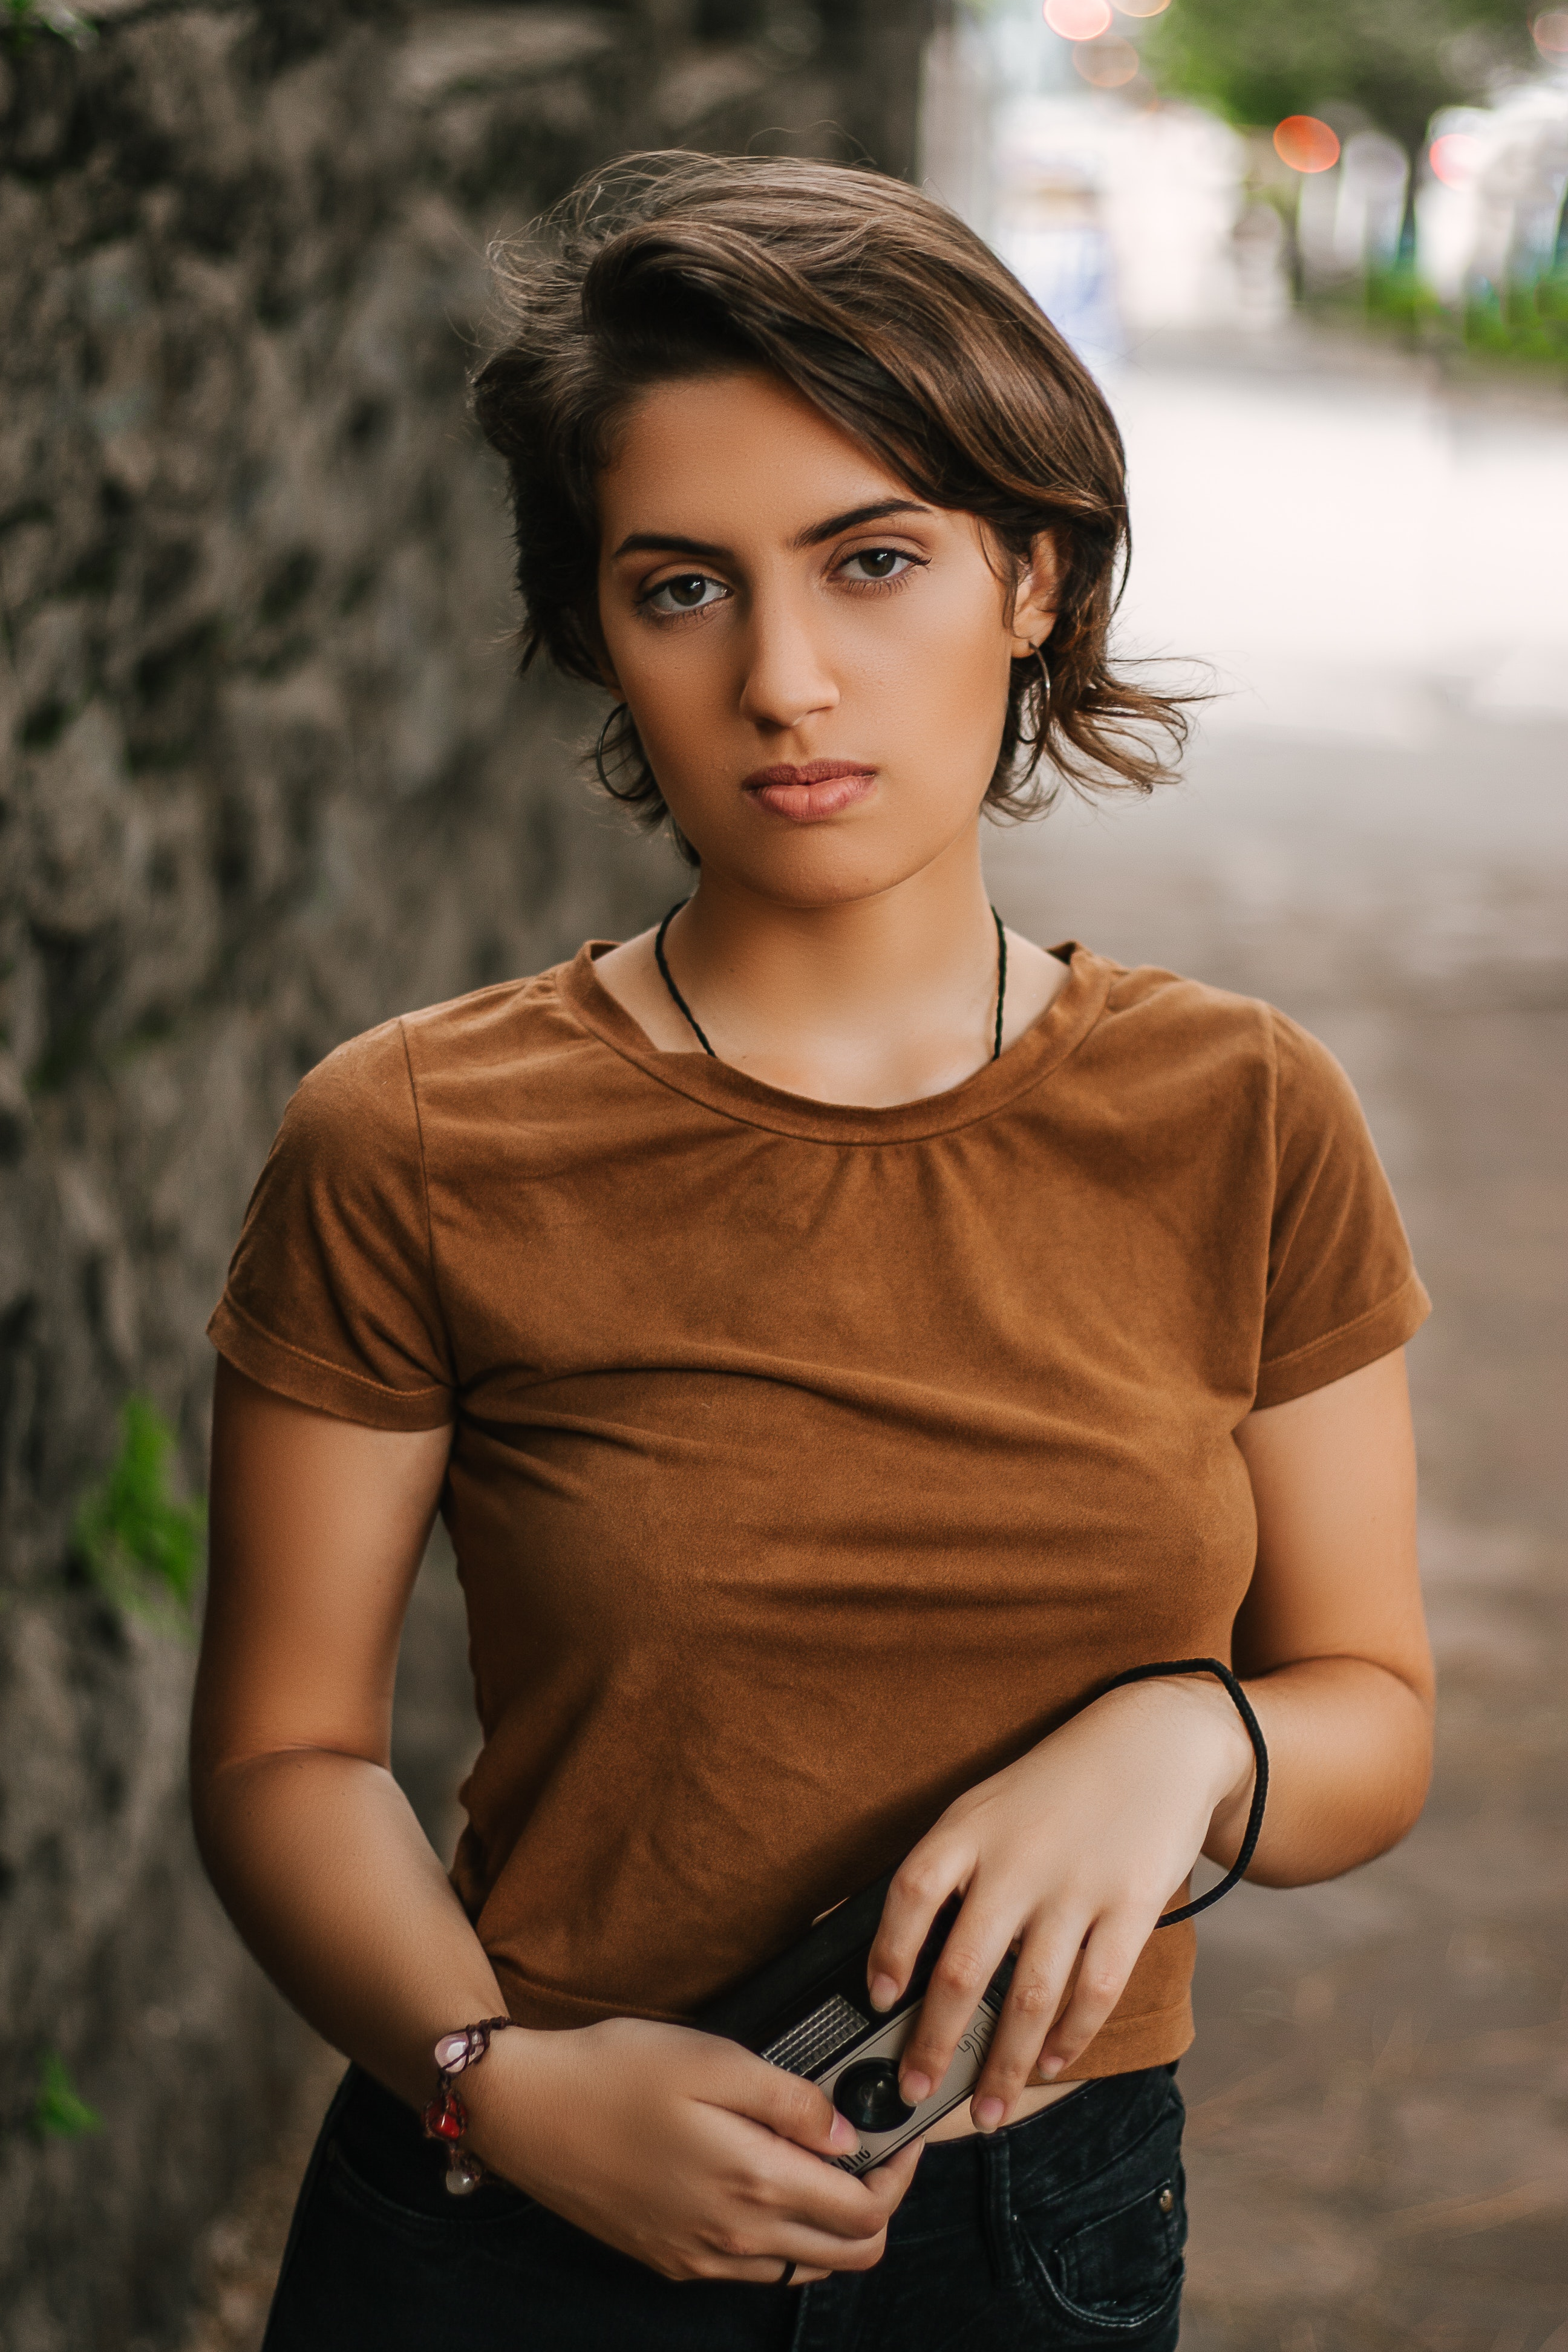
\includegraphics[width=0.9\linewidth]{images/girl_School.jpg} 
\label{fig:wrapfig}
\end{wrapfigure}

\textbf{Persona for user story 'iGo Registration'}
\\\\
\textbf{Person Name}: Vanessa Abrams 
\\\\
\textbf{Job/Role Description}: University student major in Painting and Drawing (BFA). She studies virtually approach to painting and drawing, from traditional oil painting to graphic novel production and 3D spatial installation.
\\\\
\textbf{Goals}: Use the iGo system to simplify the opus card relevant operation, and save the time for recharge.
\\\\
\textbf{Abilities}: Vanessa is a University student and familiar with the computer operation, and get access to the Internet almost everyday at home or campus.
\\\\
\textbf{Short narrative}: Vanessa is university student Vanessa. She uses the computer almost everyday. In order to finish the school project, she needs to get some information from the website. She also uses computer to download the resources like the notes to review. Sometimes she likes to watch some movies in the weekend with her families. To recap, she is quite familiar with technology, and it is not hard for her to deal with the normal and regular operation with the computer.\\

In order to get access to the iGo system ,Vanessa visits the register page first and is notified to enter a valid email address and set a password which is defined to be more than 8 characters. For her, the operation is relatively easy and straightforward, she uses the email and set the password is a regular operation.
\clearpage

\begin{wrapfigure}{l}{0.30\textwidth}
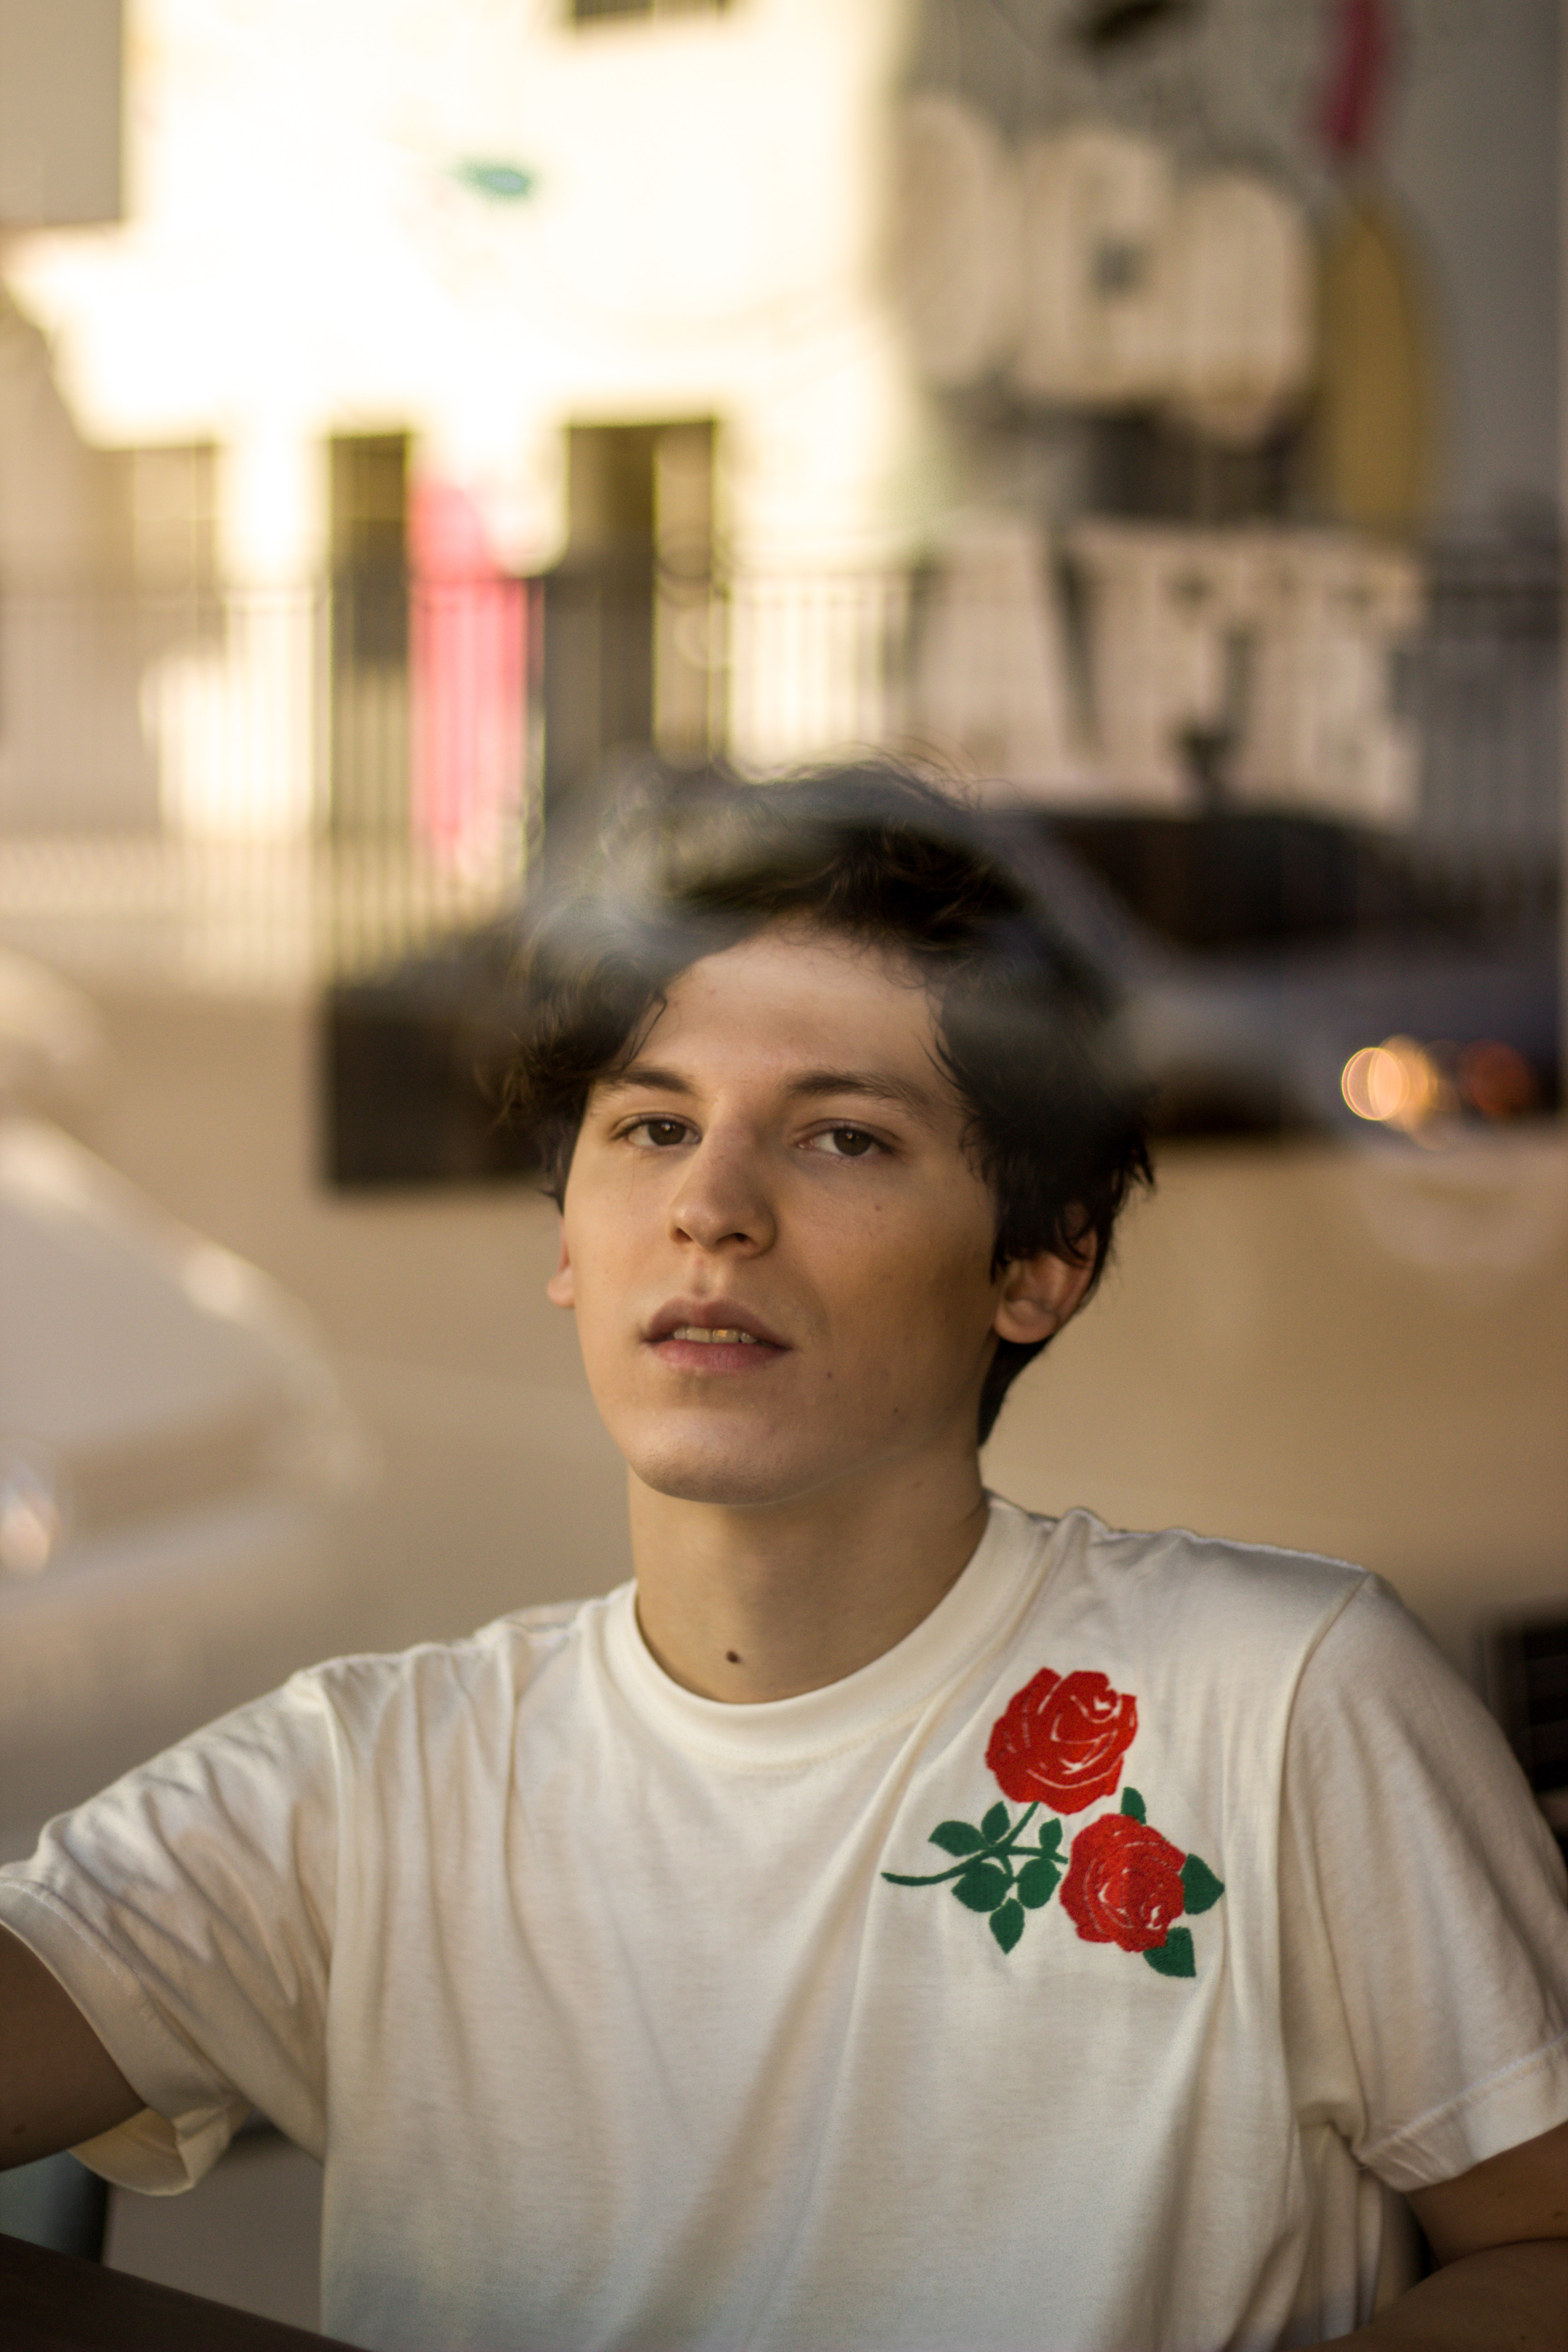
\includegraphics[width=0.9\linewidth]{images/man_Model.jpg} 
\label{fig:wrapfig}
\end{wrapfigure}

\textbf{Persona for user story 'iGo Login'}
\\\\
\textbf{Person Name}: Daniel Humphrey 
\\\\
\textbf{Job/Role Description}: He is a model for certain brand, and he has worked in the field about 2 years after he graduated from the university.
\\\\
\textbf{Goals}:Use the iGo system to simplify the card relevant operation, and save the time for recharge. His apartment is far from the working place, so the bus and the metro is the most common transportation means he uses.
\\\\
\textbf{Abilities}: Daniel likes using the Instagram to upload his photo and communicate with his friends. He likes go out with his friends in the weekend and edit the photos he captured. The 'photoshop' or some other photo editing application is his most used software.
\\\\
\textbf{Short narrative}: Daniel is also a frequent computer user, and he has the habit surfing on the internet, so the regular use and the photograph related software has no challenges for him. \\

In order to get the benefits of using the iGo system, Daniel need to get an account, and before using the service the system offered, he need to log in by entering the registered email address and the password. After the verification, Daniel is able to follow the instruction and use the system.
\\\\
\begin{wrapfigure}{l}{0.30\textwidth}

\includegraphics[width=0.9\linewidth]{images/man_Music.jpg} 
\label{fig:wrapfig}
\end{wrapfigure}
\textbf{Persona for user story 'Link OPUS card with iGo'}
\\\\
\textbf{Person Name}: Charles Bass, 
\\\\
\textbf{Job/Role Description}: He is a 
Freelancer, and he is a big fan of various kind of music, sometimes he has live show in the pub with his band.
\\\\
\textbf{Goals}:The show for the bar do not have a regular occasion. They will attend the activity if they receive the invitation from the pub or bar. In his daily life, the public transportation is the most frequently used way.
\\\\
\textbf{Abilities}: Charles always use the social application to get contact with his friends.He likes listening to the music and watching movies online. Every week, he prefers to go out with his friend to the banlieue or some small towns not too far to find some inspiration. He likes writing lyrics and create the melody himself. He uses the software like editing the music and recording.
\\\\
\textbf{Short narrative}: Charles likes surfing on the internet, So he is familiar with the operation and common process with the computer and get access to the internet. \\

In order to link the Opus card with the iGo system. Charles need to know the Opus card identification number and enter the valid email address. Definitely, the prerequisite of using the iGo system is the registration. Therefore, registering in the system is still needed.
\\\\
\\\\
\begin{wrapfigure}{l}{0.30\textwidth}

\includegraphics[width=0.9\linewidth]{images/woman_Editor.jpg} 
\label{fig:wrapfig}
\end{wrapfigure}
\textbf{Persona for user story 'Unlink OPUS card with iGo'}
\\\\
\textbf{Person Name}: Blair Waldorf, 
\\\\
\textbf{Job/Role Description}: She is an editor of the fashion design magazine. She has a good taste with cloths and interior designer.
\\\\
\textbf{Goals}: She is an occasional user for the public transportation. Since she has a car, but when she needs to attend the party or the weather is bad, she prefers to take the bus or metro. Withe the help of the online system, she is able to simplify the transaction process.
\\\\
\textbf{Abilities}: Blair likes to watch films acted by Audrey Hepburn. In the weekend, she prefers to watch the classic movie with her boyfriend. She also prefers shopping online, and find the outfits and the models that can be used in the magazine article. She also posted the photo through the 'instagram' and watch the ‘fashionist’ vlog to get to know the latest trend. 
\\\\
\textbf{Short narrative}: Blair likes surfing on the internet, because it is the way that she get to know the fashion trend. Therefore, the internet and the web is not unadaptable to her. \\

Different from the link operation. Unlink the Opus card with the iGo system is relatively easier. Blair need to log in the system before doing anything. iGo system will definitely make sure the user do the operation not accidently and prevent user making mistakes.
\clearpage

\begin{wrapfigure}{l}{0.30\textwidth}

\includegraphics[width=0.9\linewidth]{images/man_developer.jpg} 
\label{fig:wrapfig}
\end{wrapfigure}
\textbf{Persona for user story 'View OPUS card balance in iGo'}
\\\\
\textbf{Person Name}: Darshan Patel. 
\\\\
\textbf{Job/Role Description}: He is graduate student and developer in the animation production company for 6 months, he uses the .net framework in his daily work.
\\\\
\textbf{Goals}: His work place is not far from his apartment, therefore he does not possess a private car. But in the weekend, sometimes he will go out with friends and go shopping to the Downtown area. 
\\\\
\textbf{Abilities}: Darshan always use the social application to get contact with his friends to talk about the game. He likes learning the tutorial online to learn the new animation technology. Every week, he prefers to go out with his friend to have a BBQ party. He likes self-learning and come out with new ideas.
\\\\
\textbf{Short narrative}: From Darshan's perspective, being a developer makes him really familiar with various computer online operation, even the advanced operation is not difficult for him. He can be generalized as expert user. \\

View the balance in the OPUS is a service provided by iGo system, Cyrus need to log in the system before doing the relevant operation. The function is really straightforward.\\



\begin{figure}[H]
\textbf{Persona for user story 'Reset password in iGo'}
\\\\
  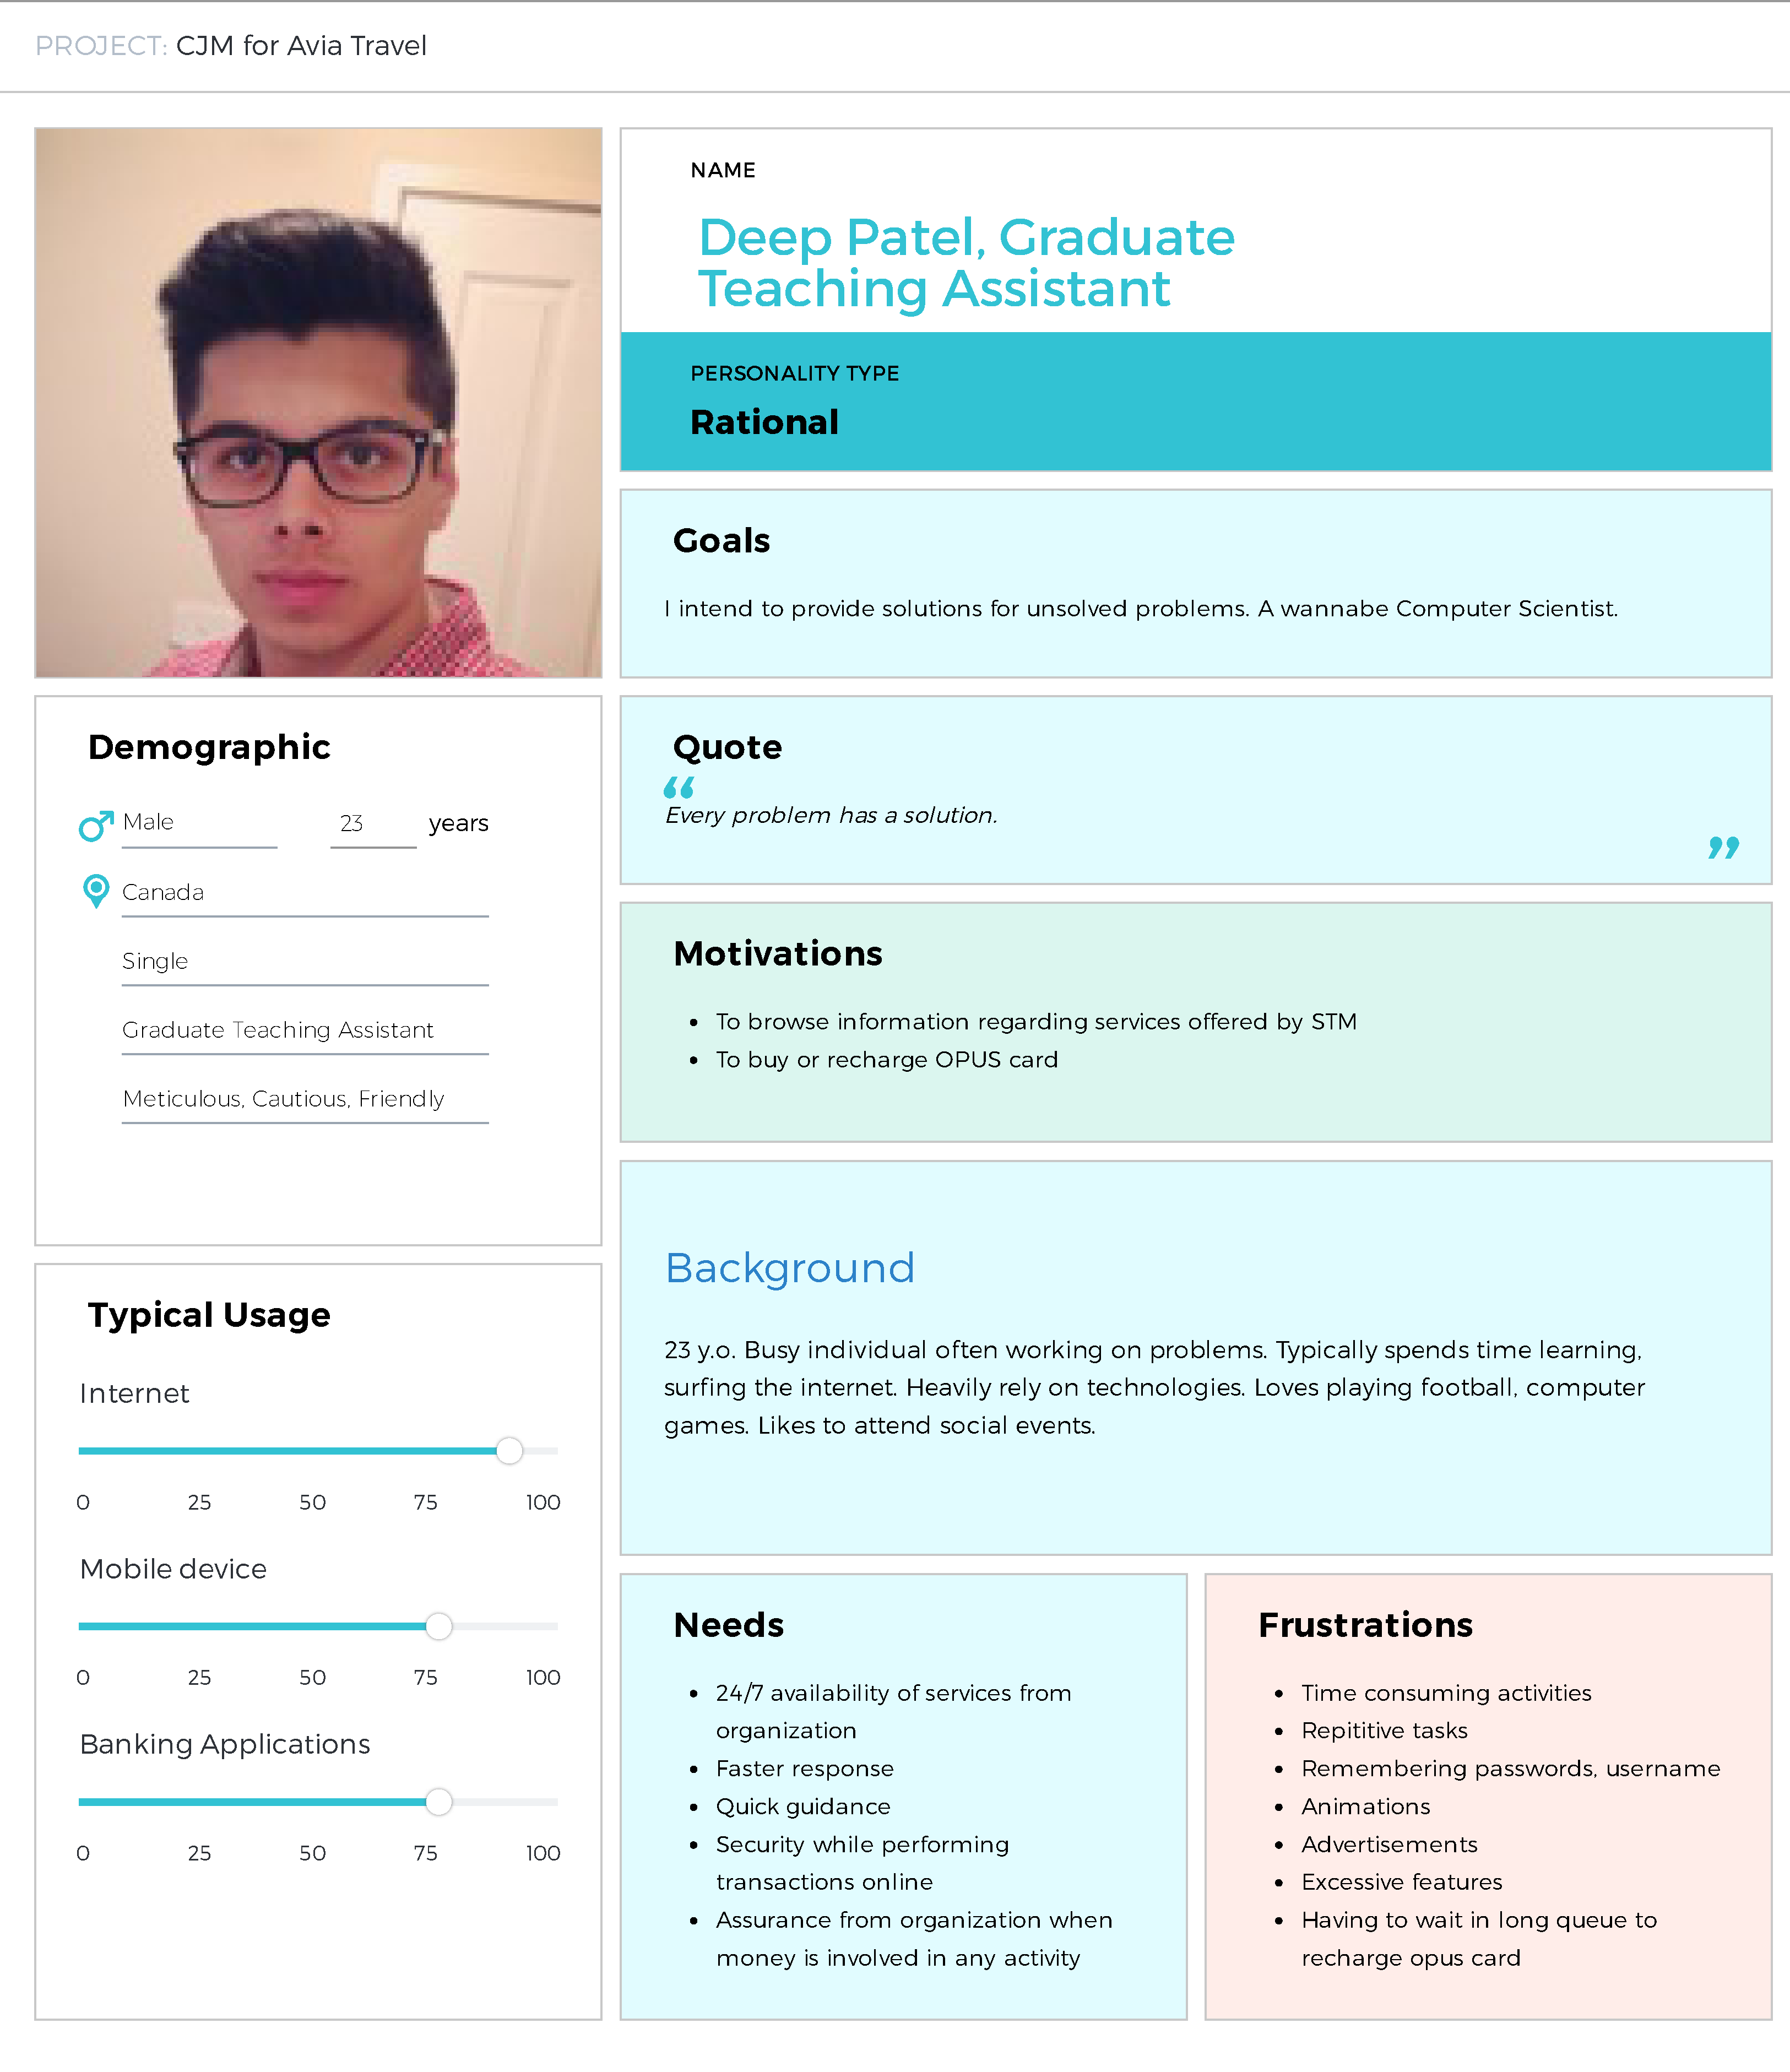
\includegraphics[width=1\textwidth]{images/Deep Patel Overleaf.png}
  \centering
\end{figure}

\begin{figure}[H]
\textbf{Persona for user story 'Load Opus Card in iGo'}
\\\\
  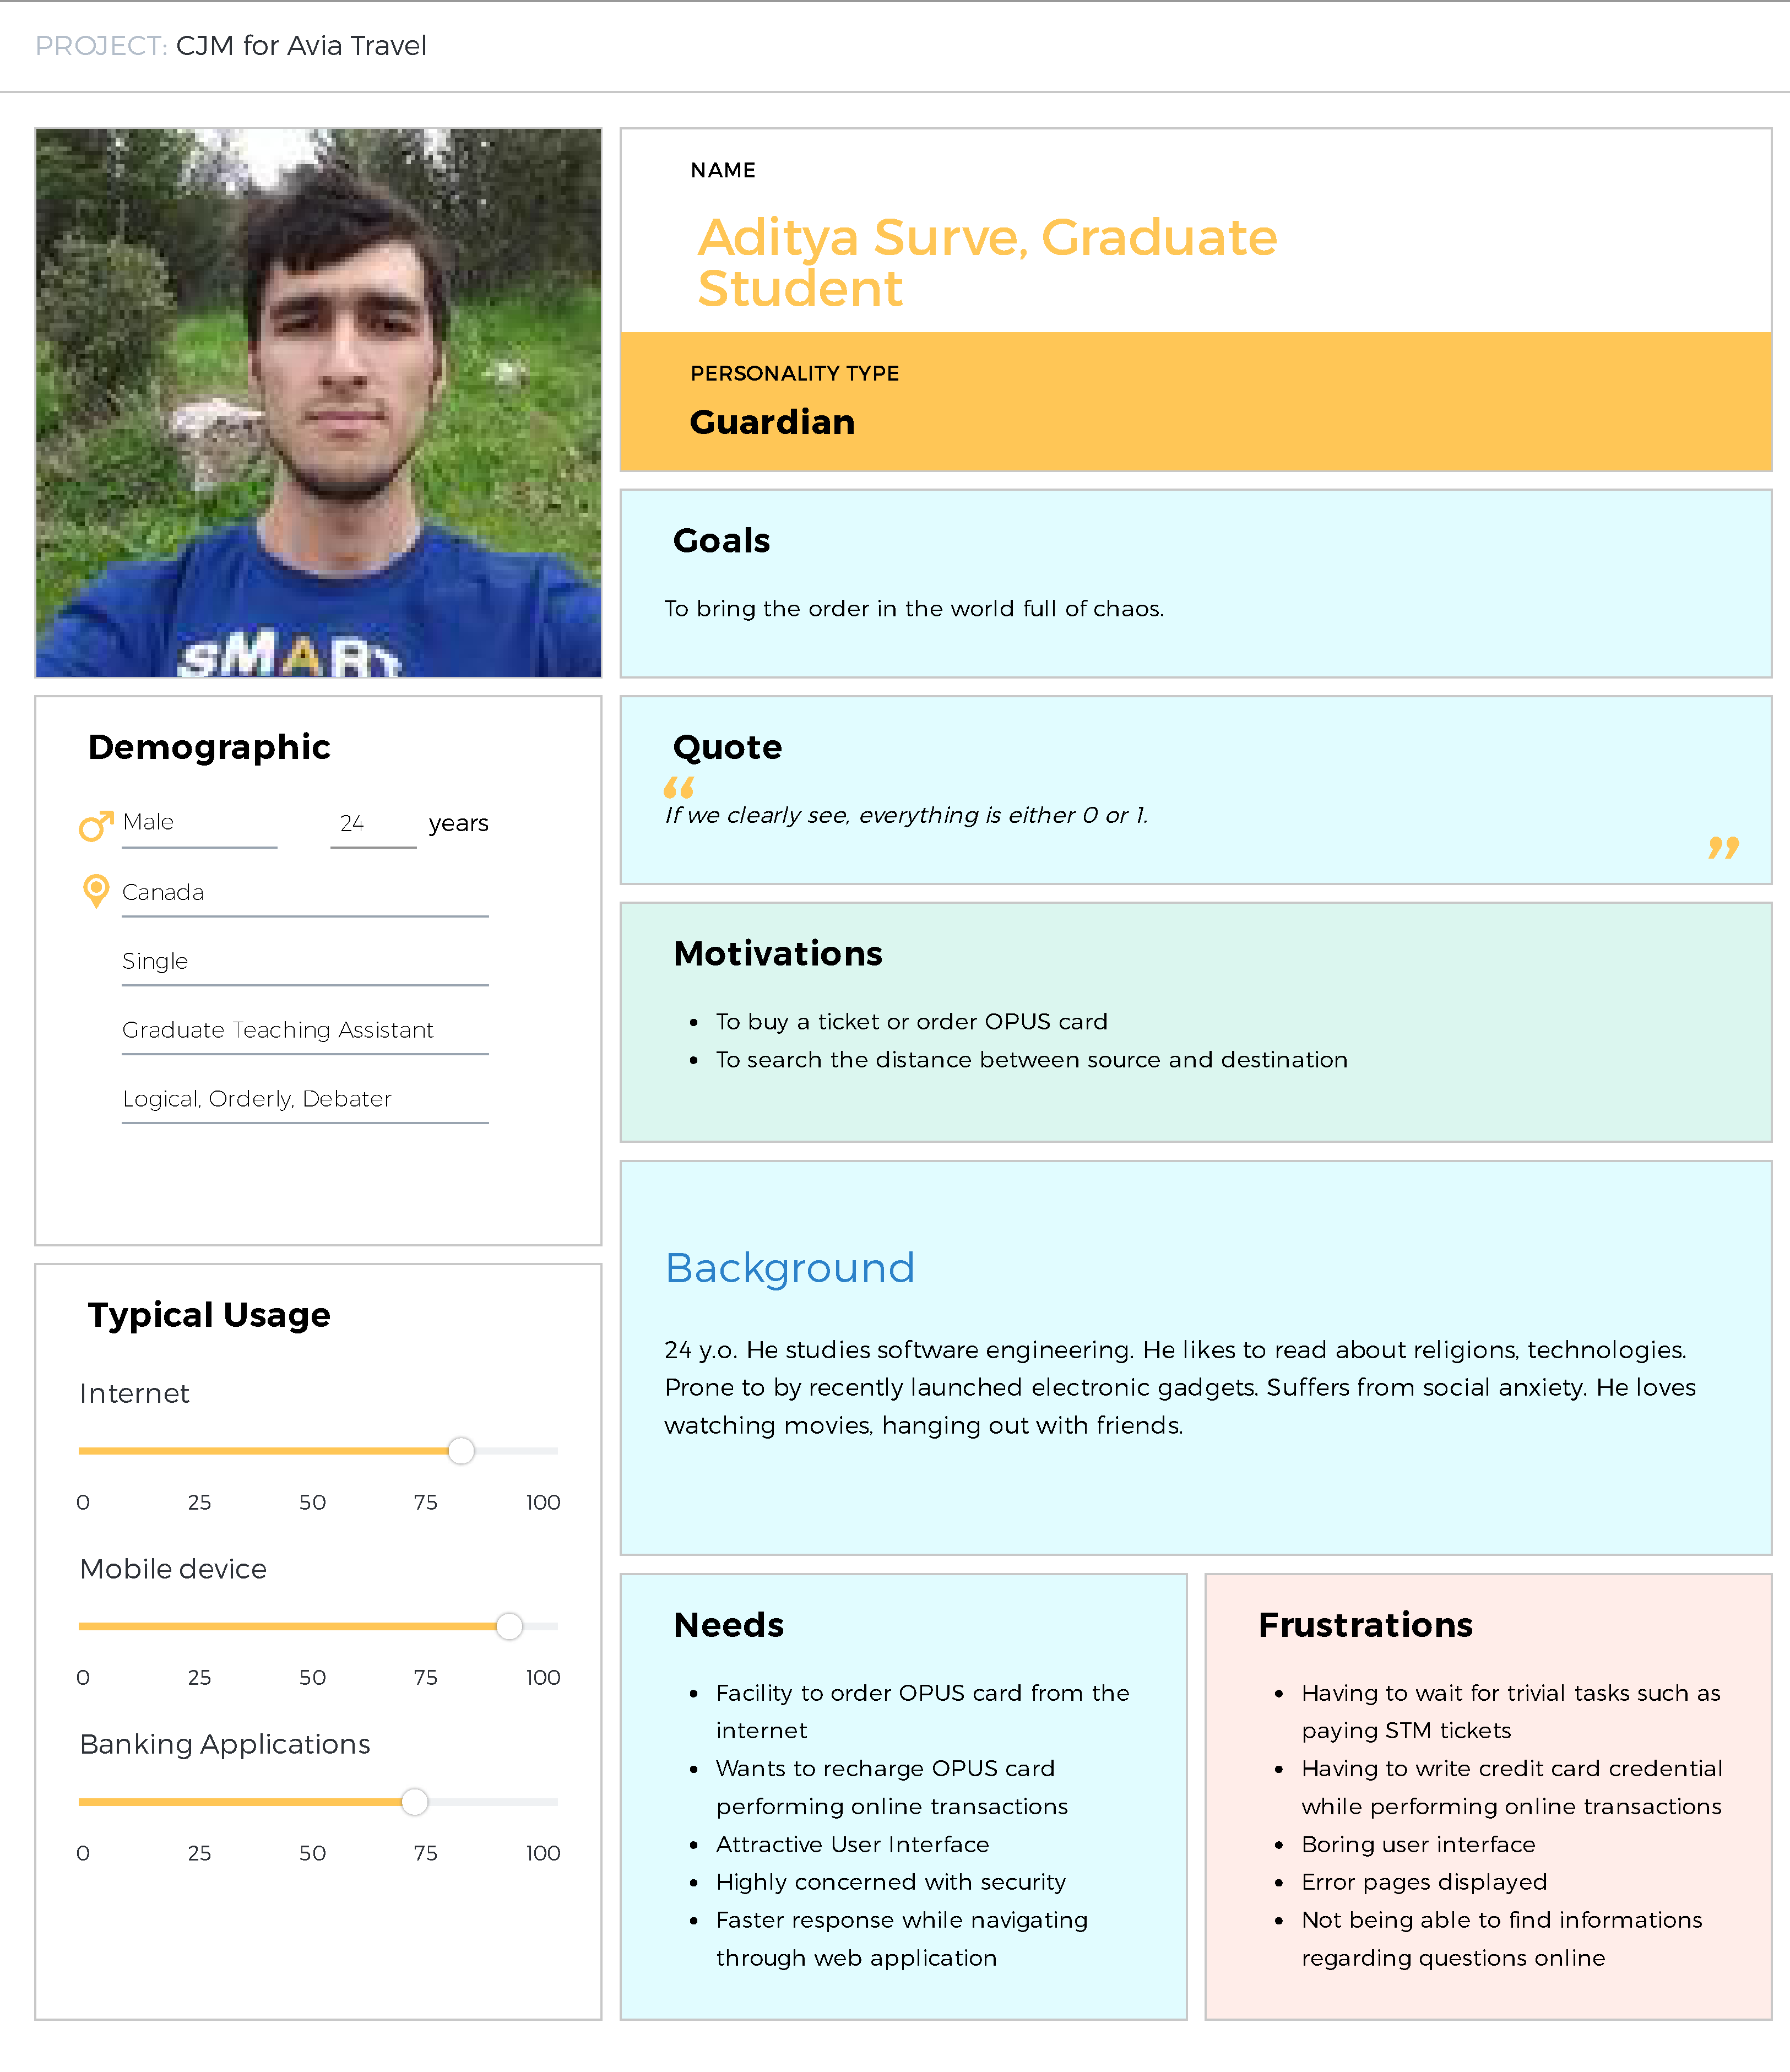
\includegraphics[width=1\textwidth]{images/Aditya Surve.png}
  \centering
\end{figure}

\chapter{Traceability Matrix }

The traceability matrix\cite{trace} of the iGo system \gls{tmigo}, is linking the requirements through the validation process. The traceability matrix is realized to ensure that all the requirements defined for the iGo system are tested and passed. The TMIGO is a table format containing the requirements and their description along with their source. TMIGO comes in handy when we need to trace the resource origin of the requirements in the long run. 

In the process of creating the traceability matrix , we have ensured that the iGo system that we are creating is on the right track. It also helps us to determine if there are any extra unspecified functionality added to the requirements. Thus, we can manage the scope of the system and keep track of how the project is affected for every change in the development lifecycle. 

\vspace*{0.2in}
\setlength{\tabcolsep}{18pt}
\renewcommand{\arraystretch}{1.5}
\begin{longtable}{ |p{0.5cm}|p{0.5cm}|p{1cm}|p{4cm}|p{2.5cm}|p{1cm}| }
\hline
\textbf{ID} & \textbf{\gls{reqid}} & \textbf{\gls{reqtype}} & \textbf{\gls{reqdesc}} & \textbf{\gls{reqsrc}} & \textbf{\gls{flag}}\\
\hline
1A& 
1&
\gls{fn}& 
Register with valid email creating email address&
iGo system description in D1&
Passed
\\
\hline
2A&
2&
FN&
Creating new account with previously registered email address& 
REQ ID 1&
Passed\\
\hline
3A&
3&
FN&
Login into the iGo system with registered email address& 
REQ ID 1&
Passed\\
\hline
4A&
4&
FN&
Invalid login&
REQ ID 1&
Passed\\
\hline
5A&
5&
FN&
Reset password in case of wrong input credentials&
User request in interview&
Passed\\
\hline
6A&
6&
FN&
Send reset password link via email to reset the password if the user forgets password&
User request in interview&
Passed\\
\hline
7A&
7&
FN&
Link OPUS card to the iGo system&
REQ ID 2&
Passed\\
\hline
8A&
8&
FN&
View OPUS card bal- ance& 
REQ ID 3 &
Passed\\
\hline
9A&
9&
FN&
Unlink the OPUS card from the iGo system&
REQ ID 5 &
Passed\\
\hline
10A&
10&
FN&
Reload OPUS card via Visa/Master card& 
REQ ID 4 &
Passed\\
\hline
\end{longtable}


\chapter{Implementation}

\section{Introduction}


There are a set of user stories which are to be implemented by the project on iGo smart ticket vending machine. Here, the user stories that are to be implemented ensure that the quality attributes are attained by the system and the system implements all the user stories which can be used for improving the existing system. As mentioned previously, we assume that STM maintains REST API through which we can get various details regarding the customers and can perform functionalities on the database. The details contain valid information about the OPUS cards.\\

Here the technology which has been utilised by us for the purpose of the API is Java along with its tools. Moreover, for the development of User Interface, we have used the Spring Framework focuses on the MVC design pattern. The built web application is platform independent and can work on all the browsers which support HTML5 and CSS3. Lastly, the project is tested to work with various inputs and provide a desired output whenever there is an issue/error in the user input. All in all, it can be said that the system is well tested and ready to be deployed in the working environment and would fulfill all the requirements of the users.\\ \\
        

Github Link for iGo system: \url{https://github.com/niravjdn/SRS-Project}


\section{Quality Attributes}

\begin{enumerate}
    \item{\textbf{Compatibility}: Our System shall provide co-existence as it will perform its required functions efficiently while sharing a common environment and resources with other systems, without detrimental impact on any other system and it will also be inter operable so that two or more systems can exchange and use information such as vehicle catalog information etc. This has been achieved by use of bootstrap library to render app on all the browser compatibly.} 
    \item{\textbf{Usability}: This system shall be easy to use for input preparation, operation, and interpretation of output and shall provide consistent user interface standards or conventions with our other frequently used systems. It will also be easy for new or infrequent users to learn to use the system as It will provide learnability, operability, user error protection, accessibility and user interface aesthetics. Our system shall increase user confidence and satisfaction by providing user friendly navigation.
    
    \item{\textbf{Reliability} - iGo web app shall be available, accessible when required for use and operational as it is indented to operate despite the presence of hardware or software faults. Moreover, in the event of an interruption or failure, this system will recover the data directly affected and re-establish the desired state of the system. This can be achieved using persistent database.}
    
    \item{\textbf{Security}: Our system shall provide confidentiality by making data accessible only to those authorized who have access through password privacy and prevent unauthorized access and modification of data. Thus, security can be characterized as a system providing non repudiation, confidentiality, integrity, assurance, availability, and auditing. This shall be achieved using spring security as a security layer. Along with authorization, we have also provided encryption facilities which can make the system more secure.}
    
    \item{\textbf{Maintainability}: This system shall be maintainable because it is composed of discrete components such that a change to one component has minimal impact on other components. It shall also be reusable as module that is developed with high cohesion and low coupling can be used in more than one system, or building other assets. It will provide the effectiveness and efficiency with which it is possible to assess the impact on a product or system of an intended change to one or more of its parts, or to diagnose a product for deficiencies or causes of failures, or to identify parts to be modified. Moreover, it will also be effectively and efficiently modified and tested without introducing defects or degrading existing product quality. This shall be achieved by using Spring MVC.}
    
    \item{\textbf{Portability}: The system can be run on any tomcat server with minimum 128MB RAM. Hence, Considering this, System shall be portable. }
}
\end{enumerate}


\section{User Story 1,2 : Registration using email} 
As a new iGo web user, I want to create a new account on iGo website by my valid email and a secure password. So that I can use that credentails to login later on iGo website with my registered credentials.

\begin{figure}[H]
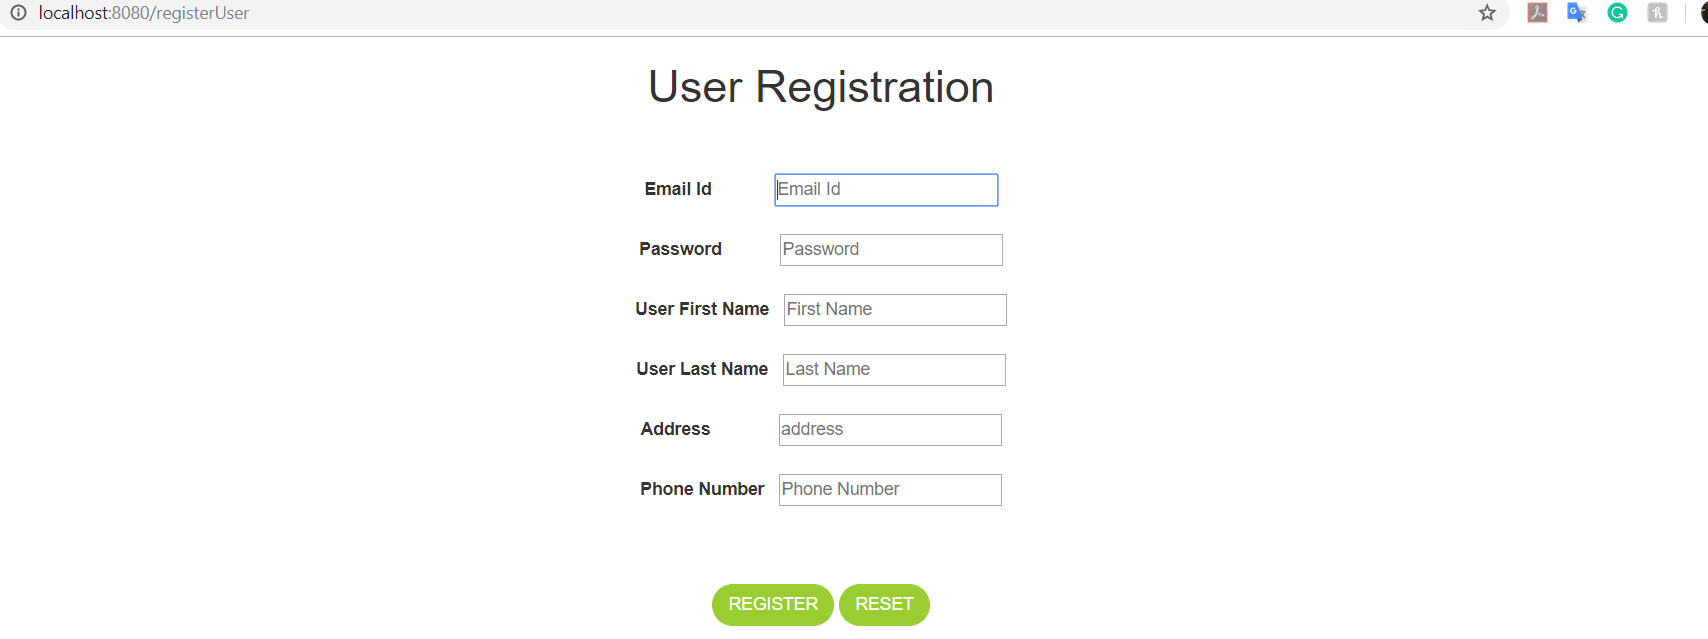
\includegraphics[width=1\textwidth]{images/UserRegistration.PNG}
  \centering
  \caption{iGo web page to let new users to register into the system
}
\end{figure}

\begin{figure}[H]
  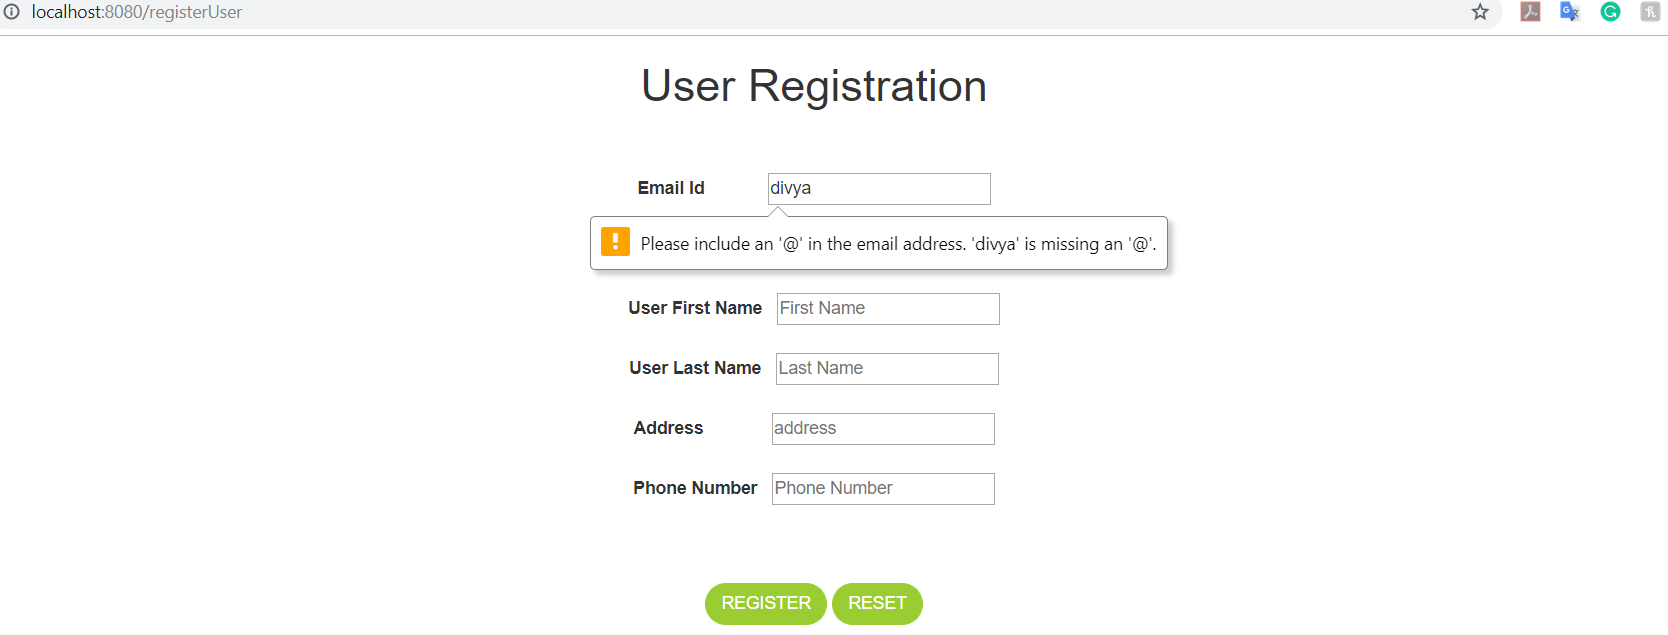
\includegraphics[width=1\textwidth]{images/InvalidEmail.PNG}
  \centering
  \caption{When user enters invalid email id format then the system will not let them create an account with iGo
}
\end{figure}

\begin{figure}[H]
  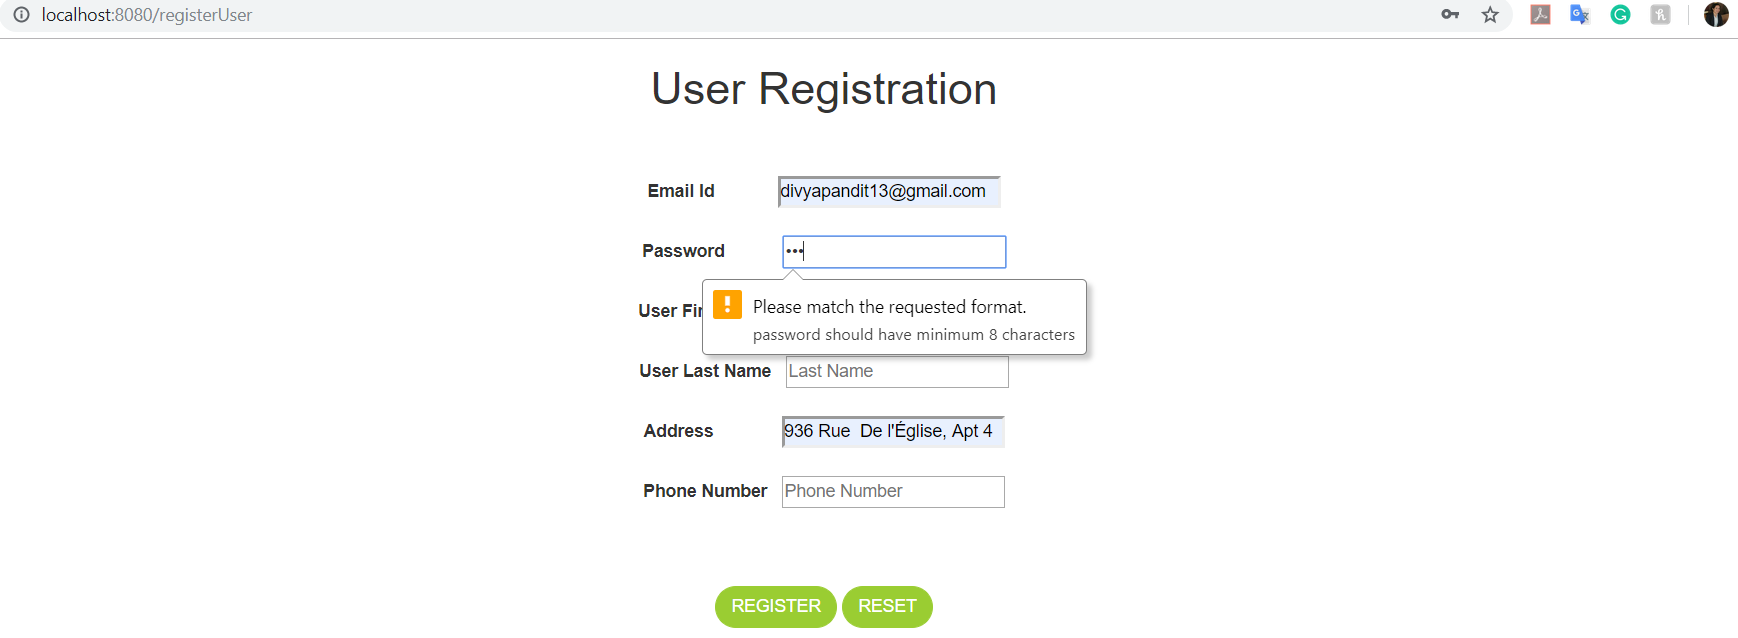
\includegraphics[width=1\textwidth]{images/InvalidPassword.PNG}
  \centering
  \caption{When the user enters a password that contains less than 8 characters, the system does not let them create an account with iGo
}
\end{figure}

\begin{figure}[H]
  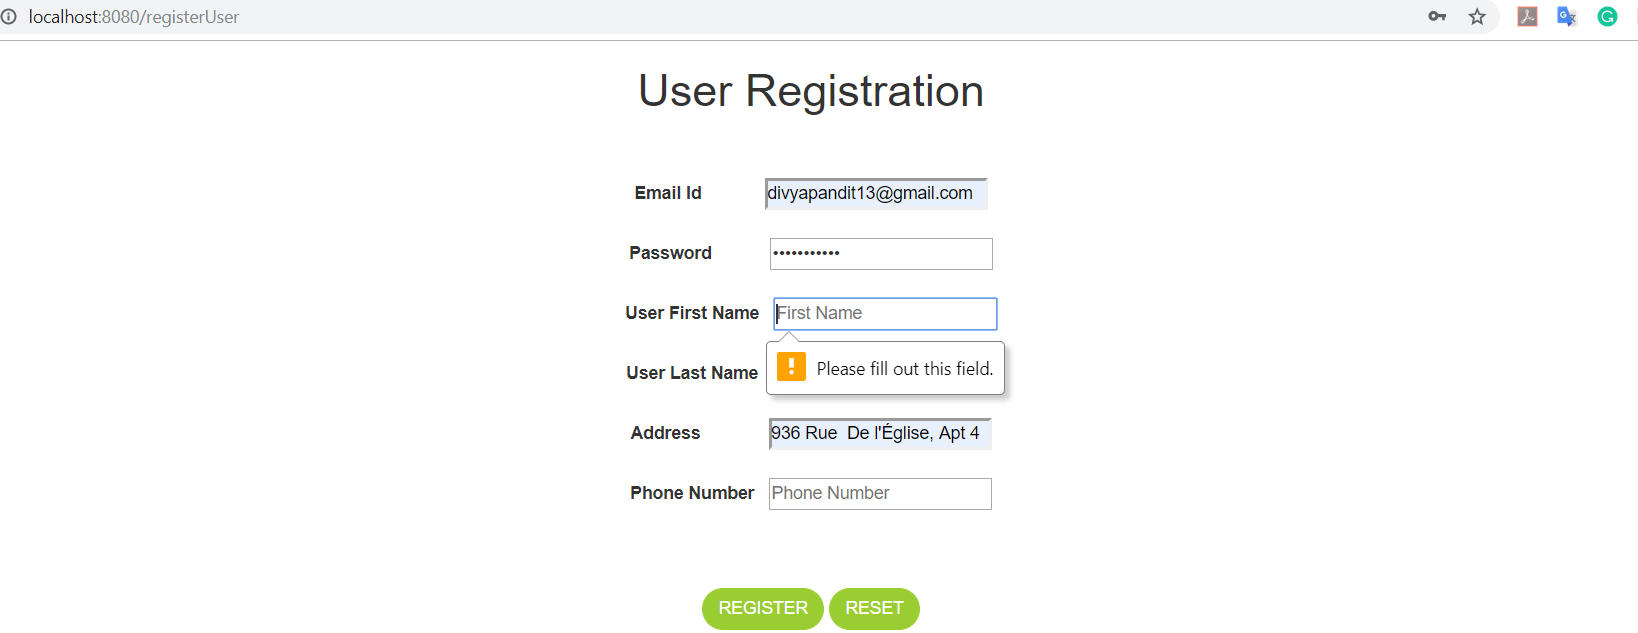
\includegraphics[width=1\textwidth]{images/Requiredname.PNG}
  \centering
  \caption{When the user needs to enter first name and last name before submitting details for new account in iGo
}
\end{figure}

\begin{figure}[H]
  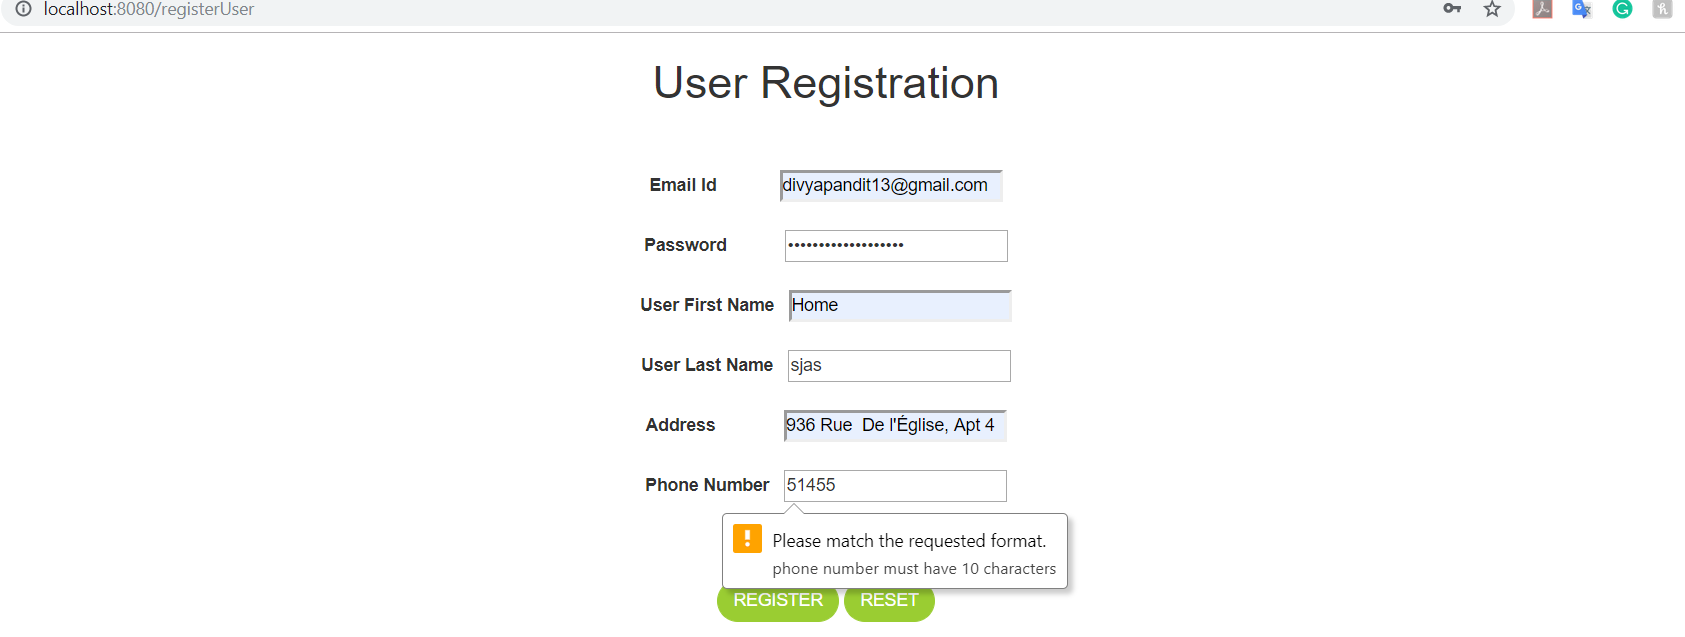
\includegraphics[width=1\textwidth]{images/ValidPhone.PNG}
  \centering
  \caption{When the user enters a phone number that is not exactly matching 10 characters (Invalid Phone Number), the system does not let them create an account with iGo
}
\end{figure}

\begin{figure}[H]
  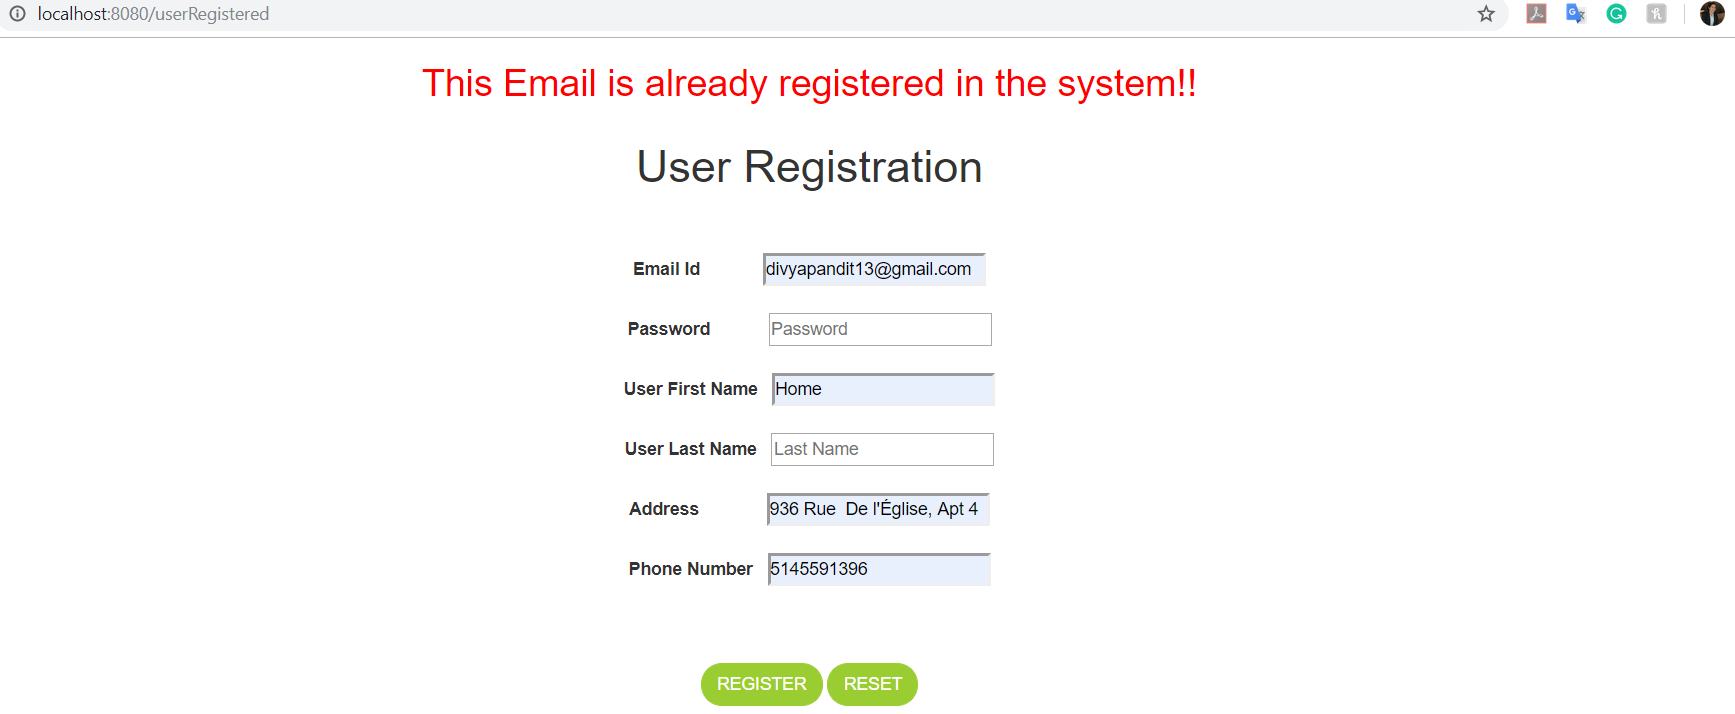
\includegraphics[width=1\textwidth]{images/EmailIdVerify.PNG}
  \centering
  \caption{When the user tries to register using email used by already existing user.}
\end{figure}


\section{User Story 3,4 : Login} 
An existing user want to login to iGo website with my registered email and password so that he/she shall be able to login to iGo website and use services offered by iGo.


\begin{figure}[H]
  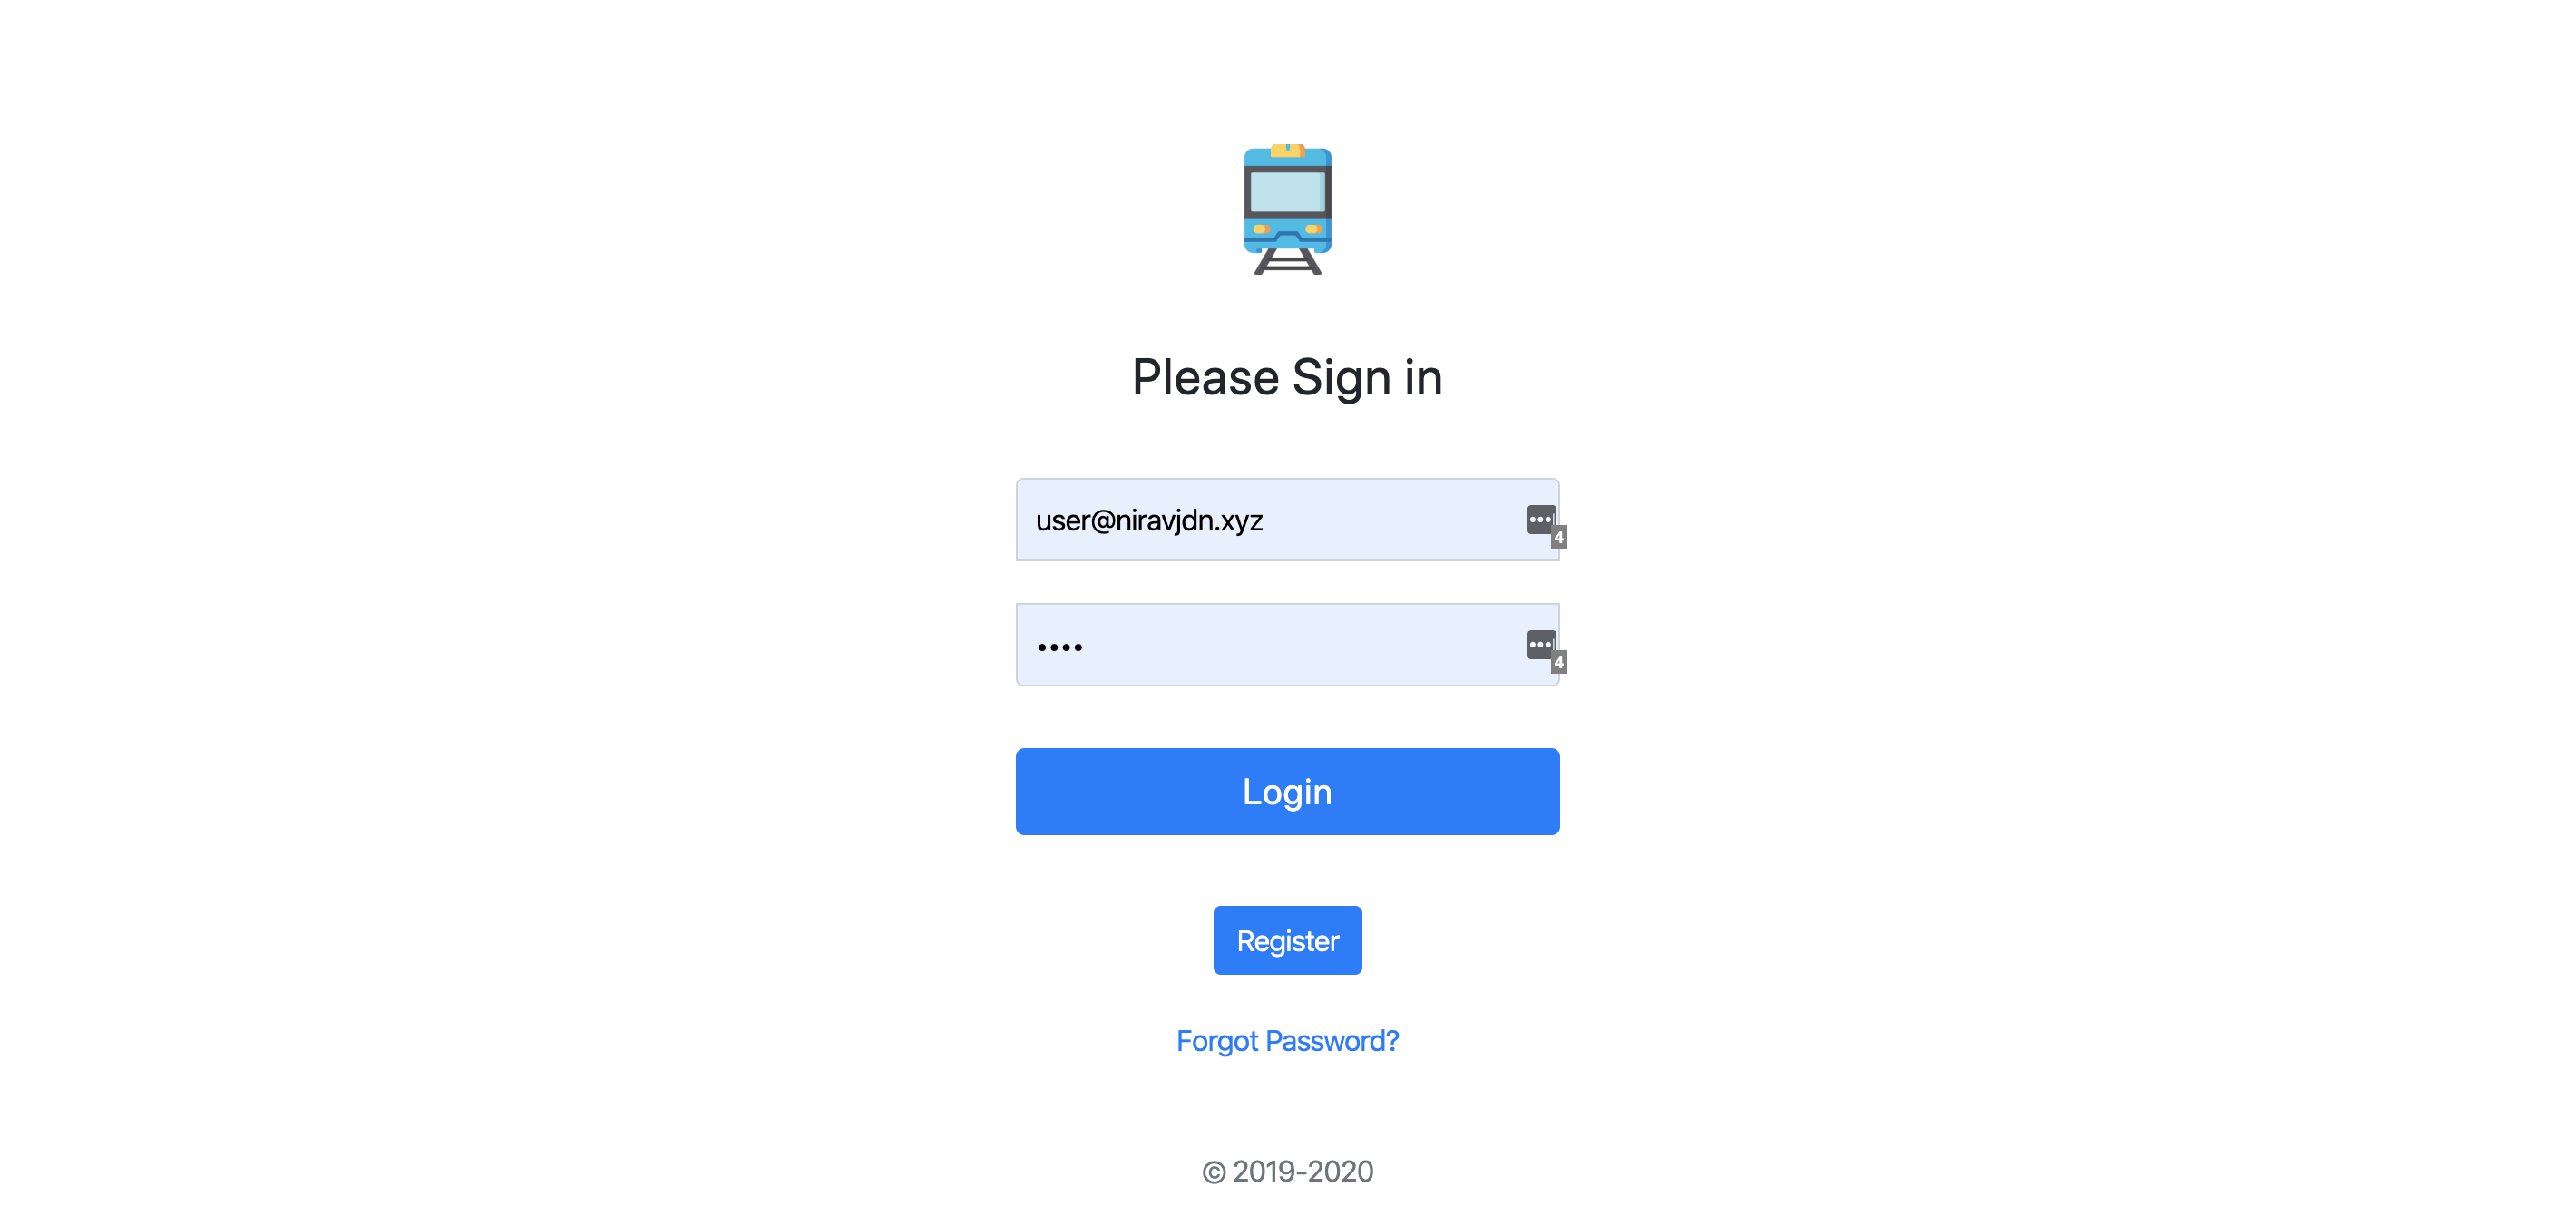
\includegraphics[width=1\textwidth]{images/login_page.png}
  \centering
  \caption{Login web page to let existing iGo user to enter valid credentials to login to the iGo system to perform various transactions
}
\end{figure}

\begin{figure}[H]
  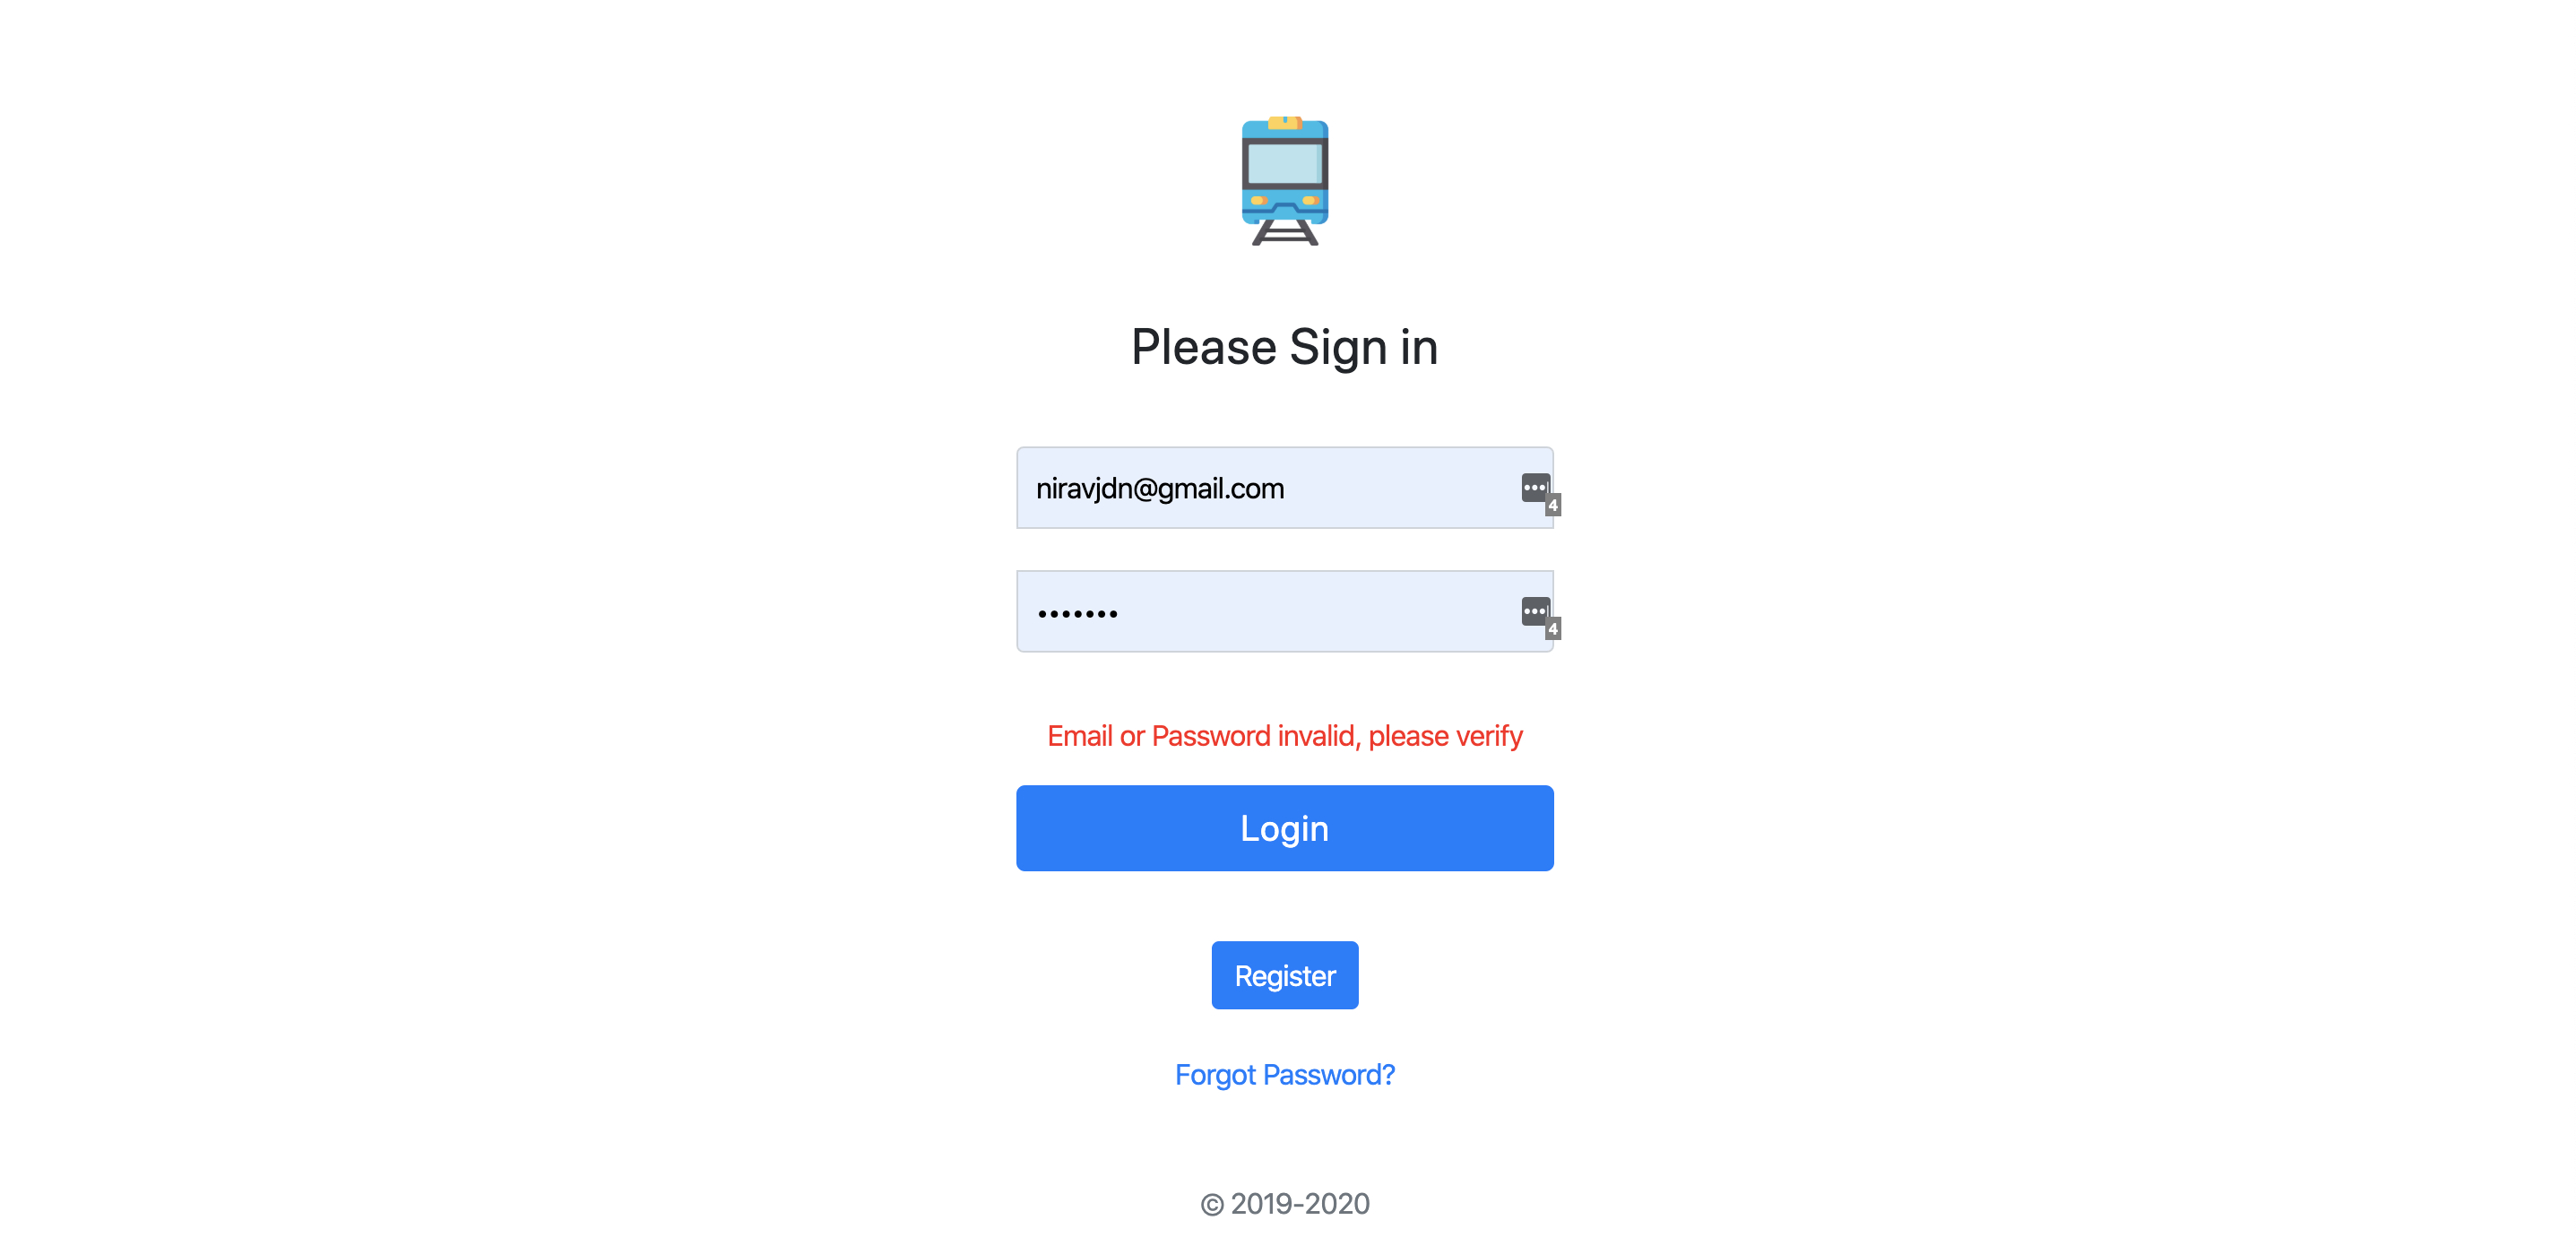
\includegraphics[width=1\textwidth]{images/invalid_credz.png}
  \centering
  \caption{When the user enters invalid credentials that does not exist in the iGo database, then the iGo does not let the user login to their account
}
\end{figure}

\begin{figure}[H]
  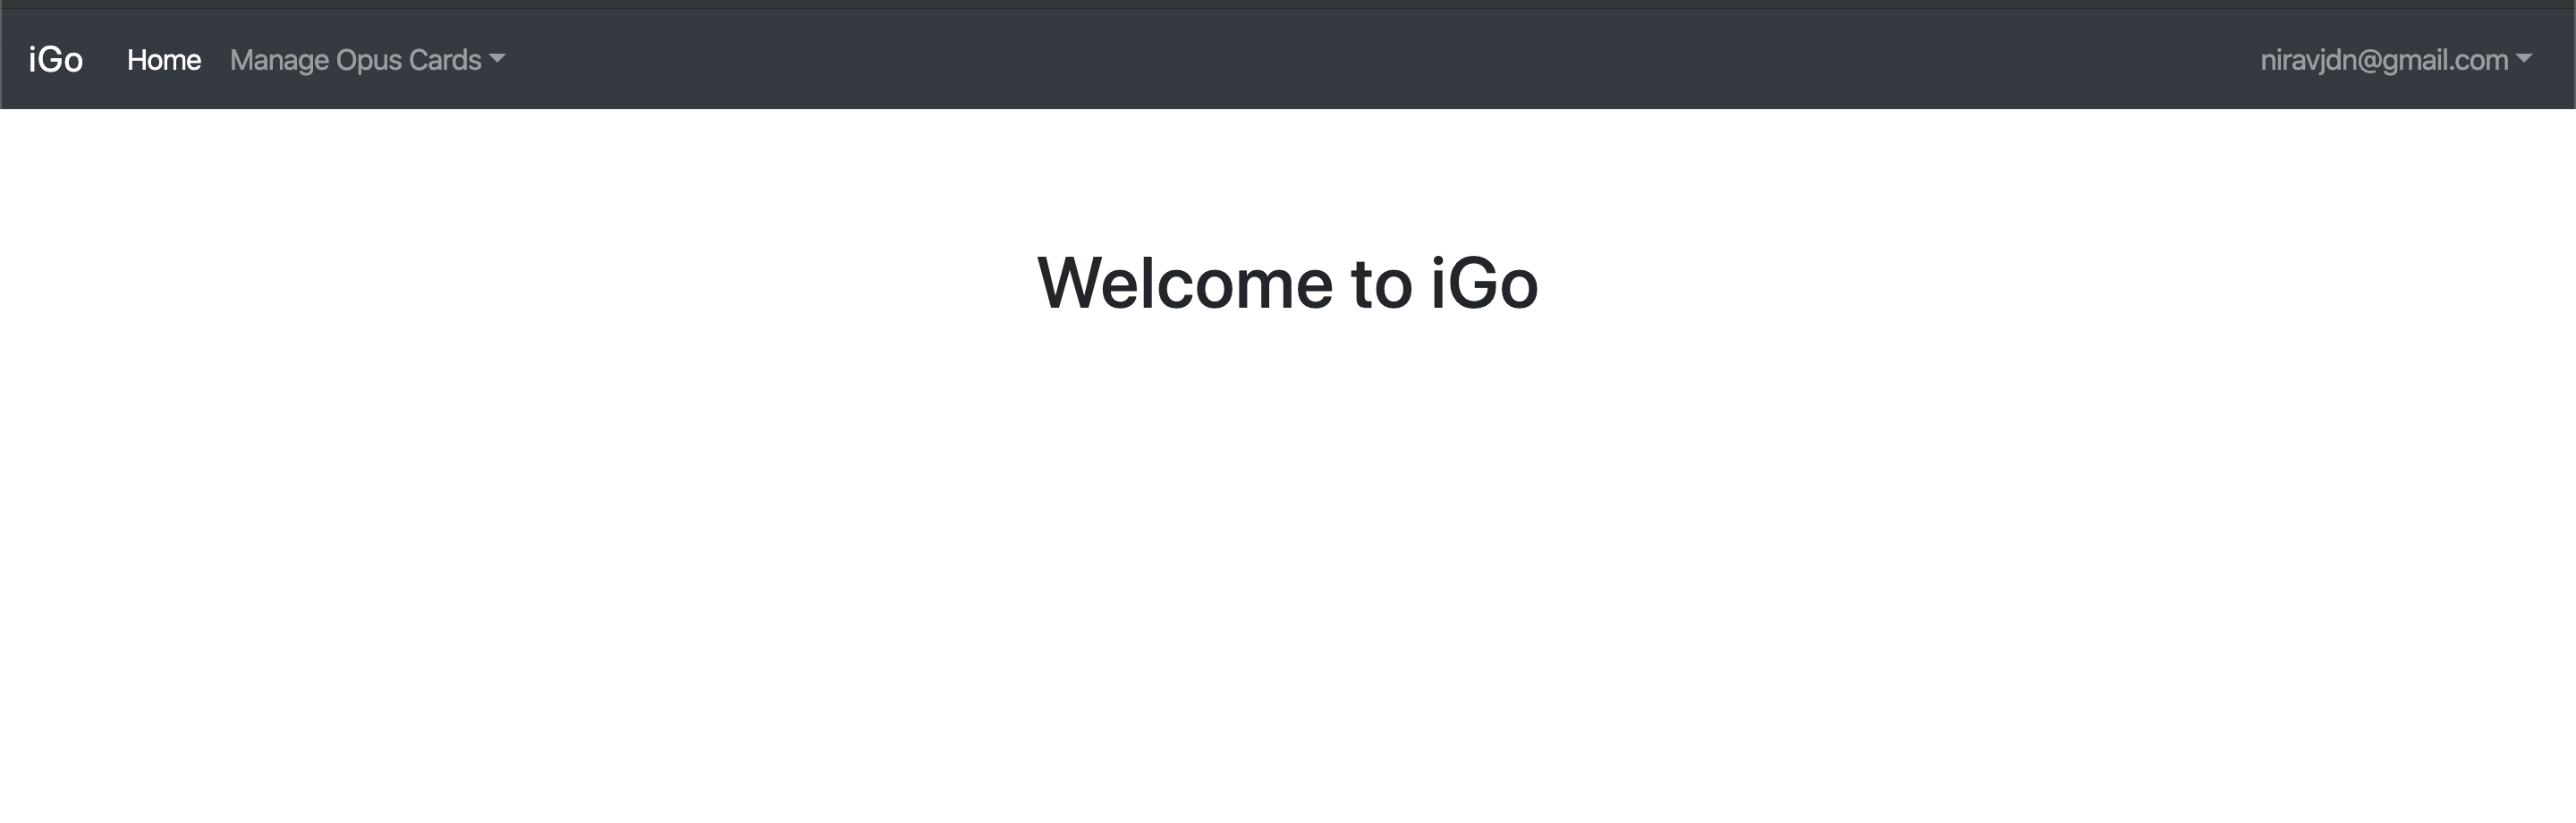
\includegraphics[width=1\textwidth]{images/login_successful.png}
  \centering
  \caption{When the user enters valid credentials that exists in the iGo database, then the iGo redirects them to the dashboard of iGo account.
}
\end{figure}


\section{User Story 5,6: Reset Password}

An Existing iGo user want to reset password. This might be possible if user has forgot the password or want to reset it.

\begin{figure}[H]
  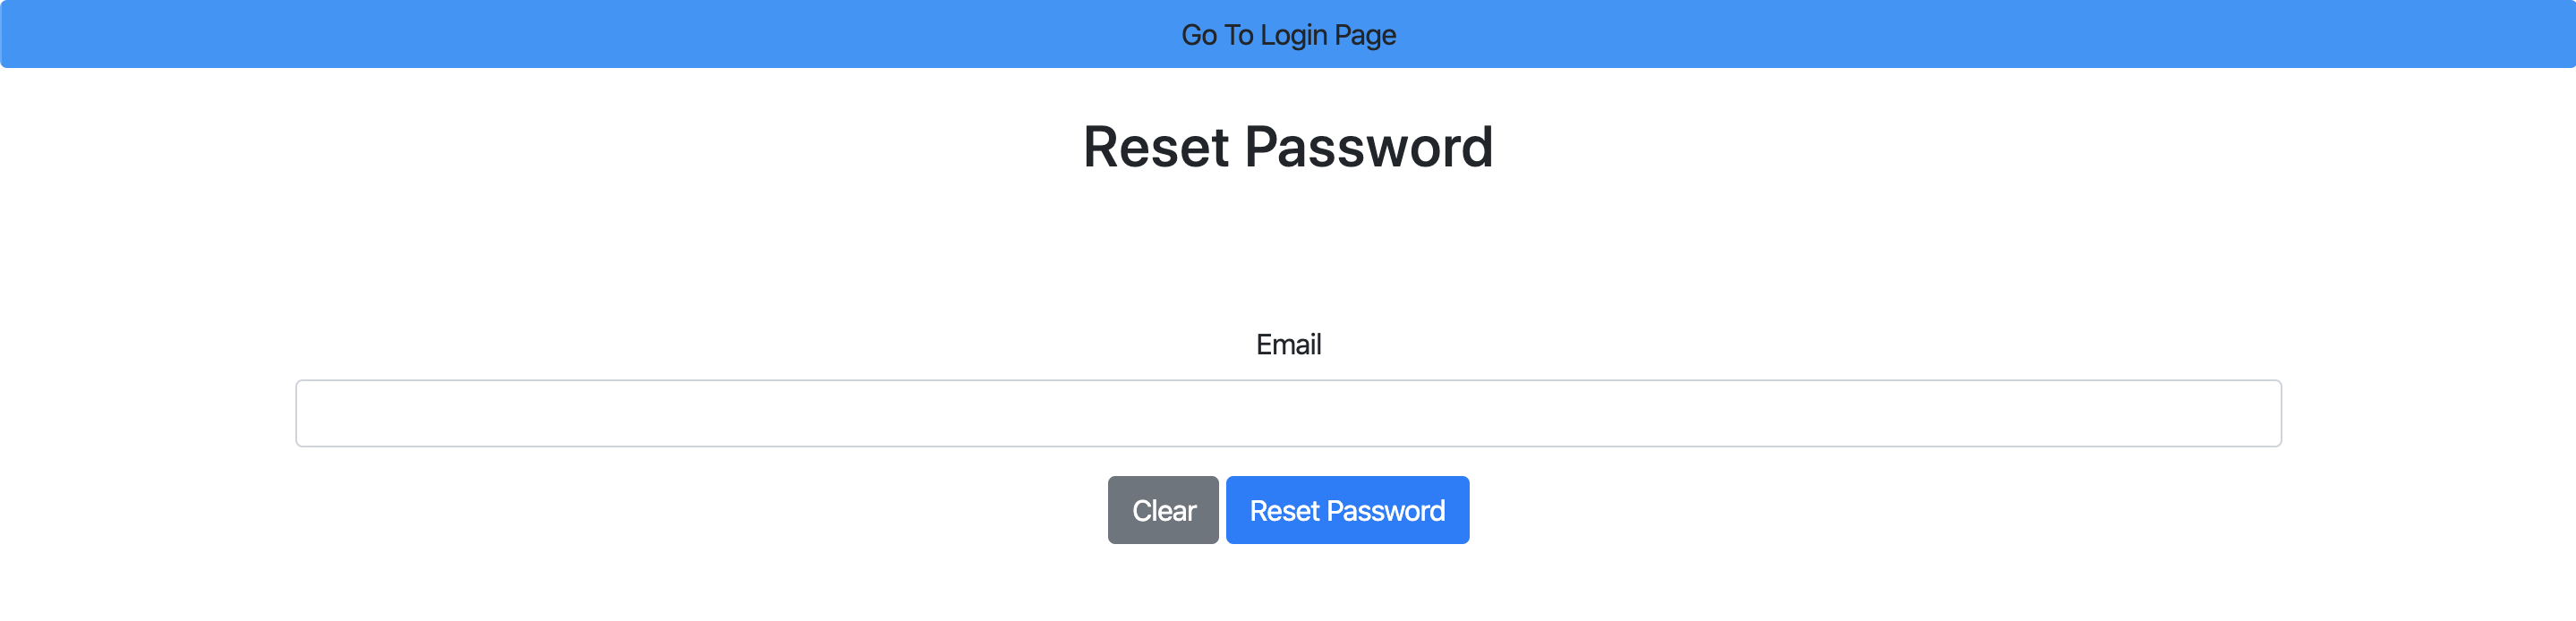
\includegraphics[width=1\textwidth]{images/reset_password_page.png}
  \centering
  \caption{Password reset page to let user enter valid email id}
\end{figure}

\begin{figure}[H]
  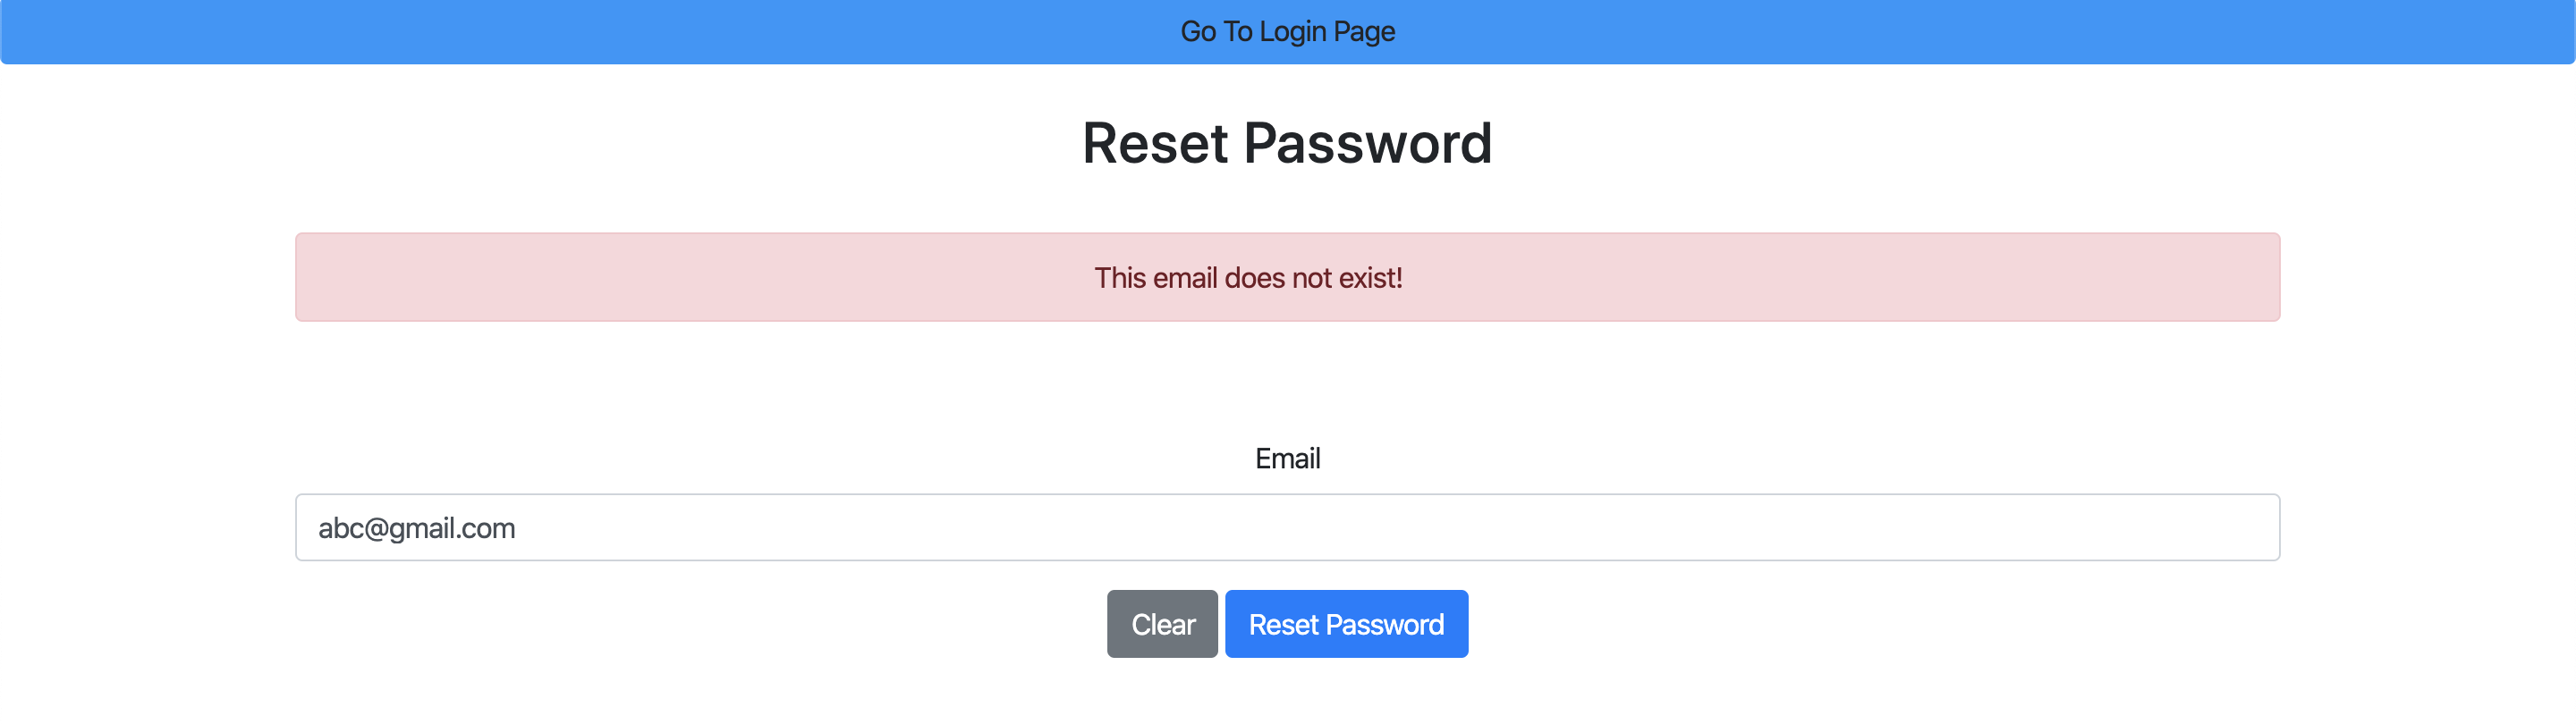
\includegraphics[width=1\textwidth]{images/invalid_email_forgot_password.png}
  \centering
  \caption{A page showing user that email does not exist if user enters invalid email which does not exist in iGo Database.}
\end{figure}


\begin{figure}[H]
  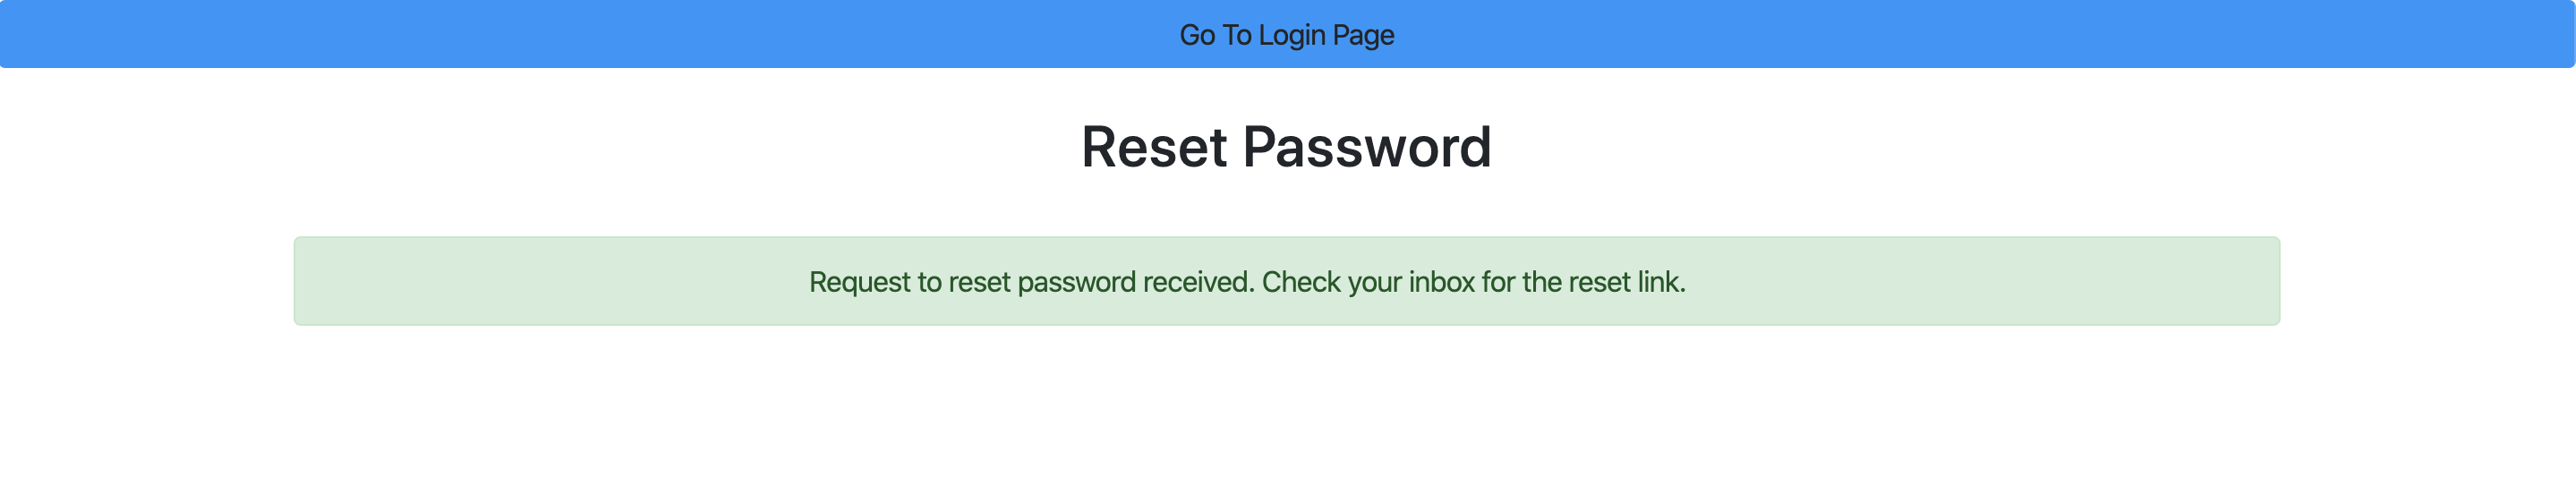
\includegraphics[width=1\textwidth]{images/reset_password_sent_message.png}
  \centering
  \caption{A page showing that password reset link has been sent to email.}
\end{figure}

\begin{figure}[H]
  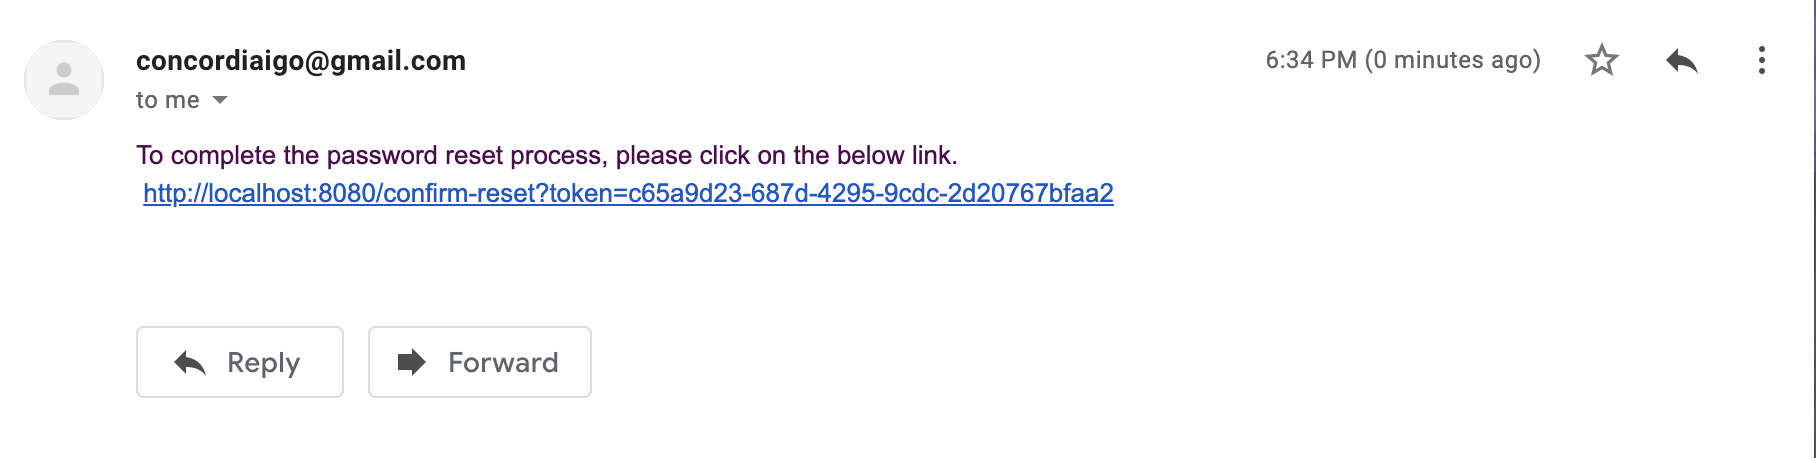
\includegraphics[width=1\textwidth]{images/reset_password_email.png}
  \centering
  \caption{An email sent by system to user with password reset link}
\end{figure}

\begin{figure}[H]
  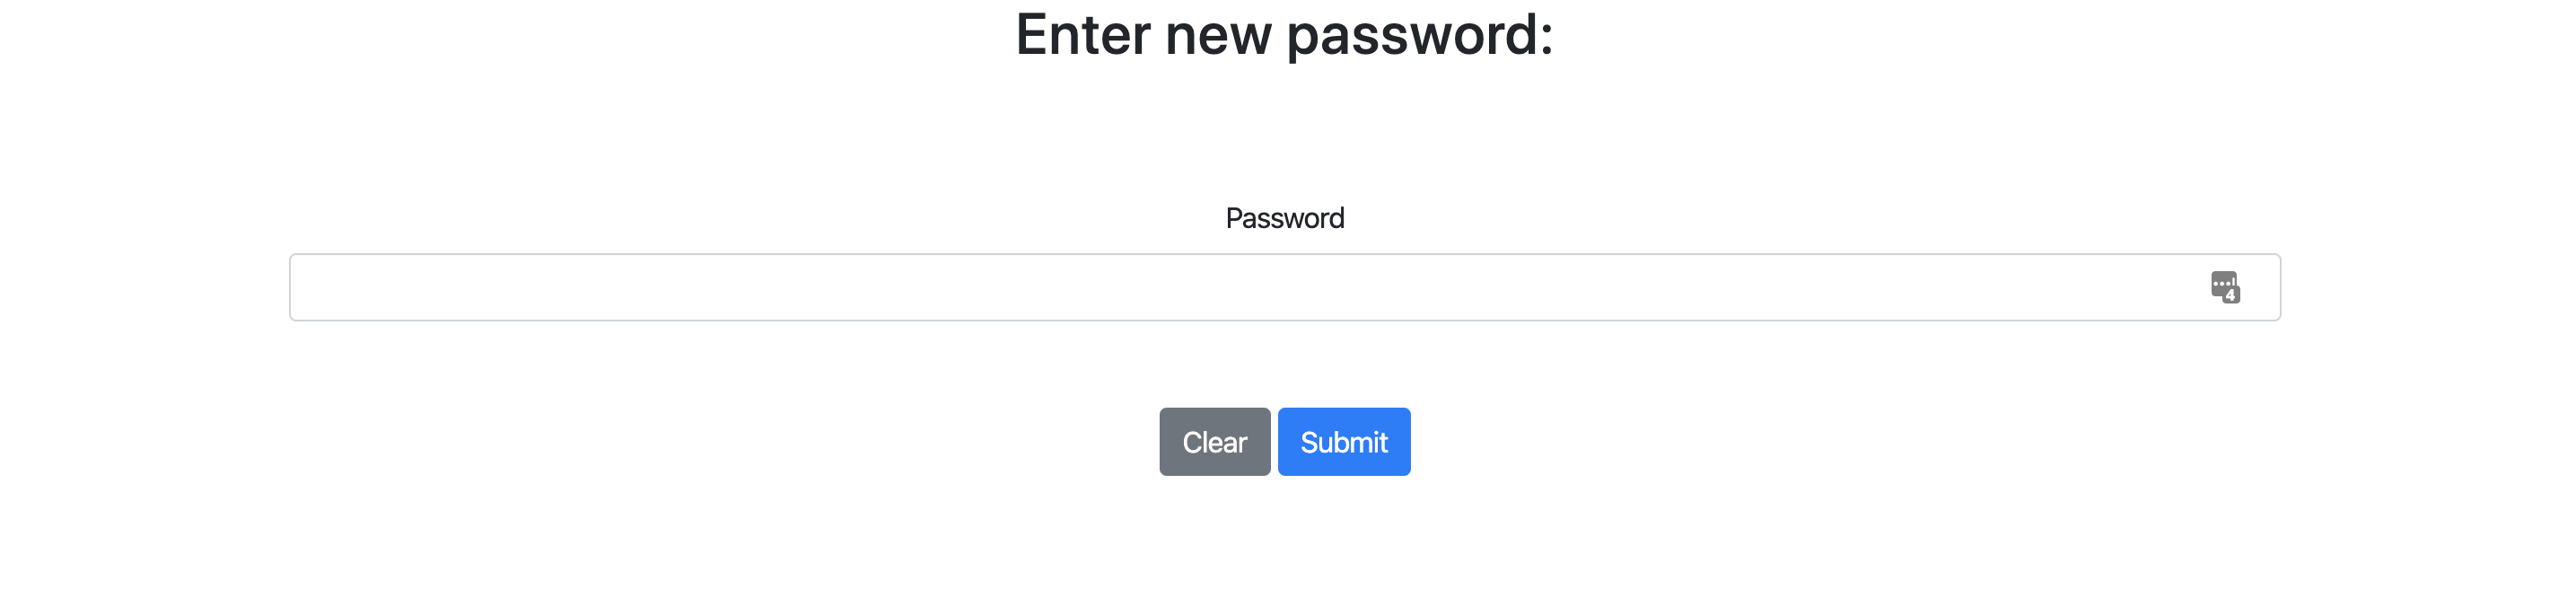
\includegraphics[width=1\textwidth]{images/reset_password_form.png}
  \centering
  \caption{A form to let user enter new password once he clicks on link received on the email}
\end{figure}

\begin{figure}[H]
  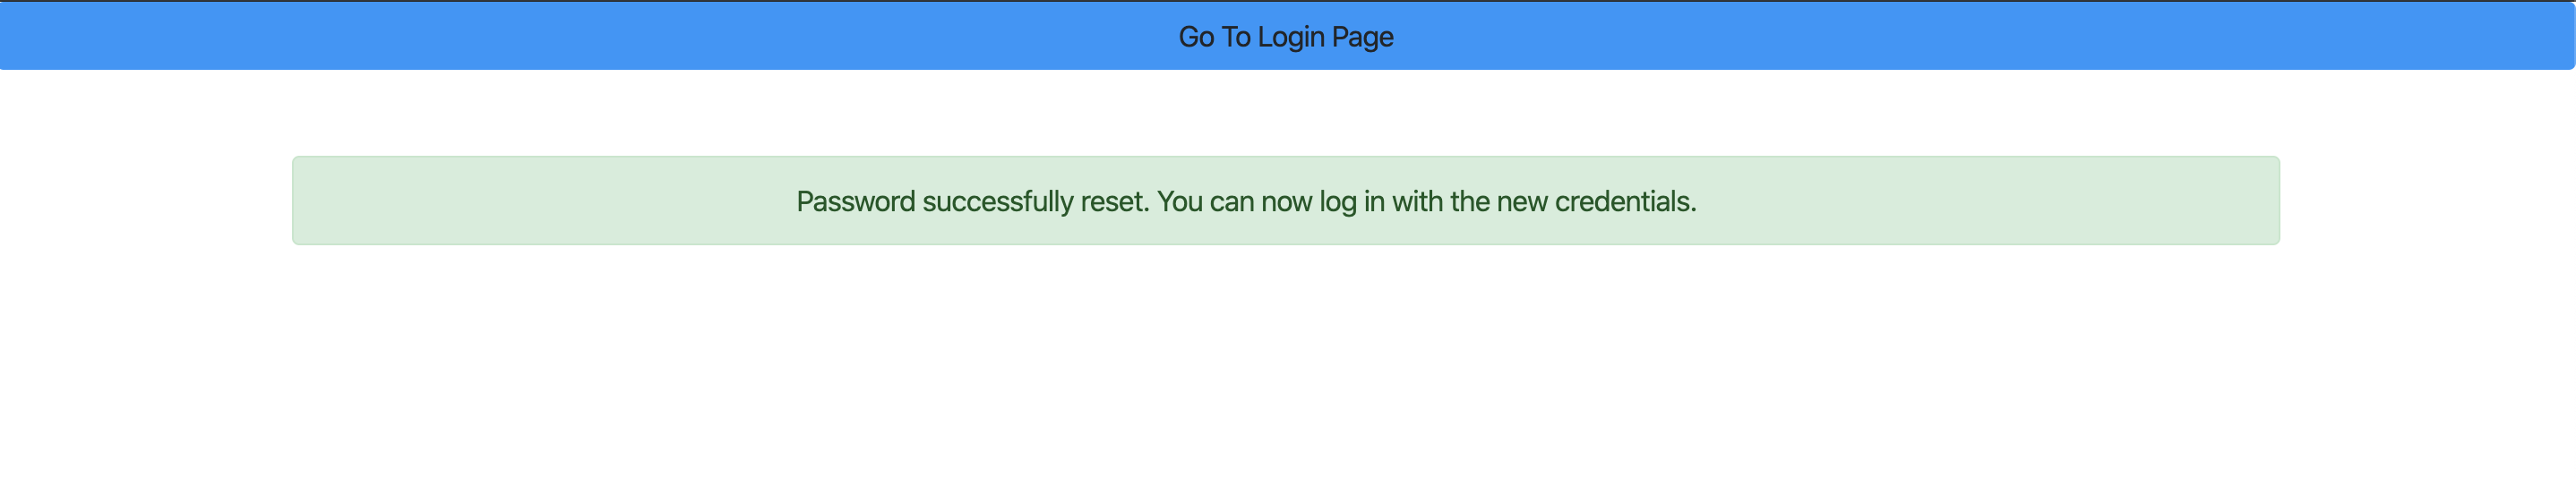
\includegraphics[width=1\textwidth]{images/password_reset_successful.png}
  \centering
  \caption{A page showing message that password reset has been successful and now user can login using new password.}
\end{figure}

\section{User story 7,8 : Link and Unlink Opus Card}

An existing iGo User want to link iGo Opus Card to his/her account. After login, the user can link and unlink opus card.

\begin{figure}[H]
  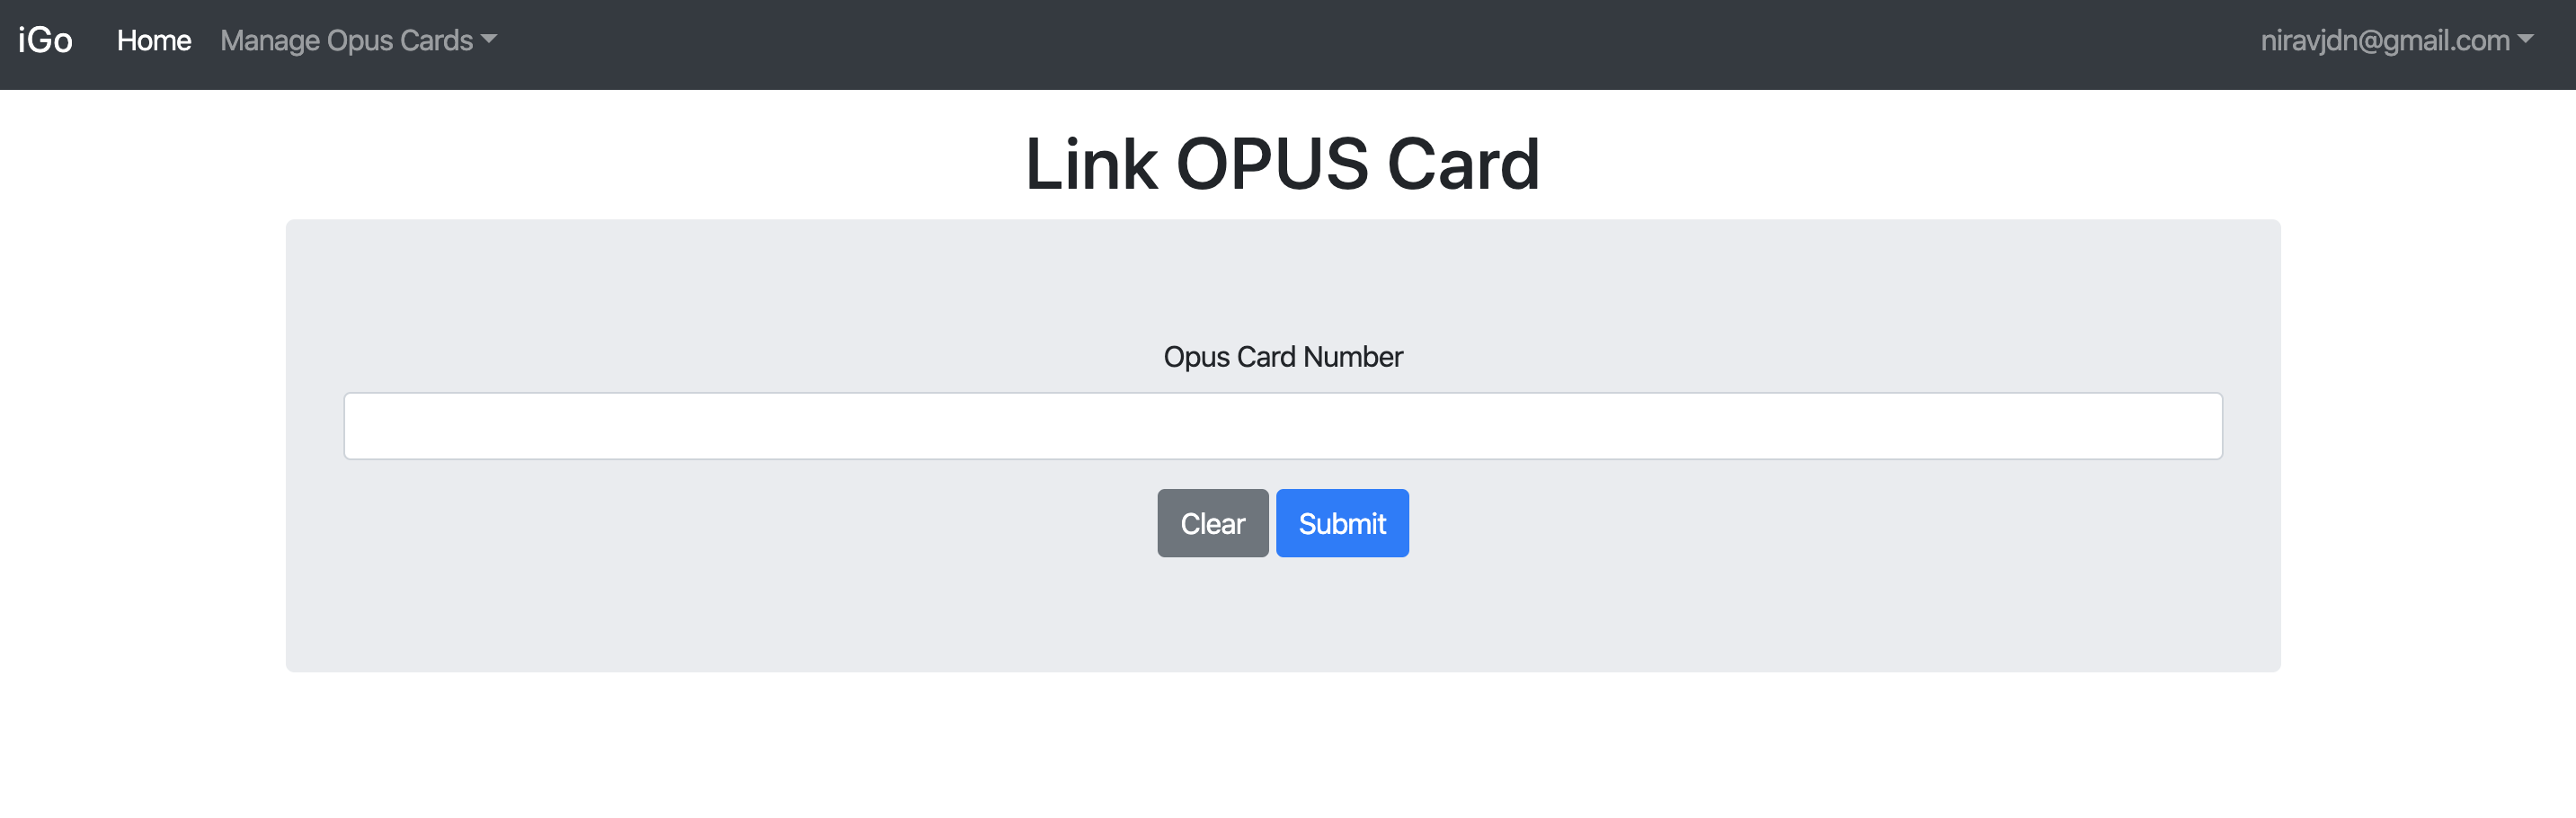
\includegraphics[width=1\textwidth]{images/link_opus_card_page.png}
  \centering
  \caption{The web page to enter opus card details to link the card to the iGo account}
\end{figure}

\begin{figure}[H]
  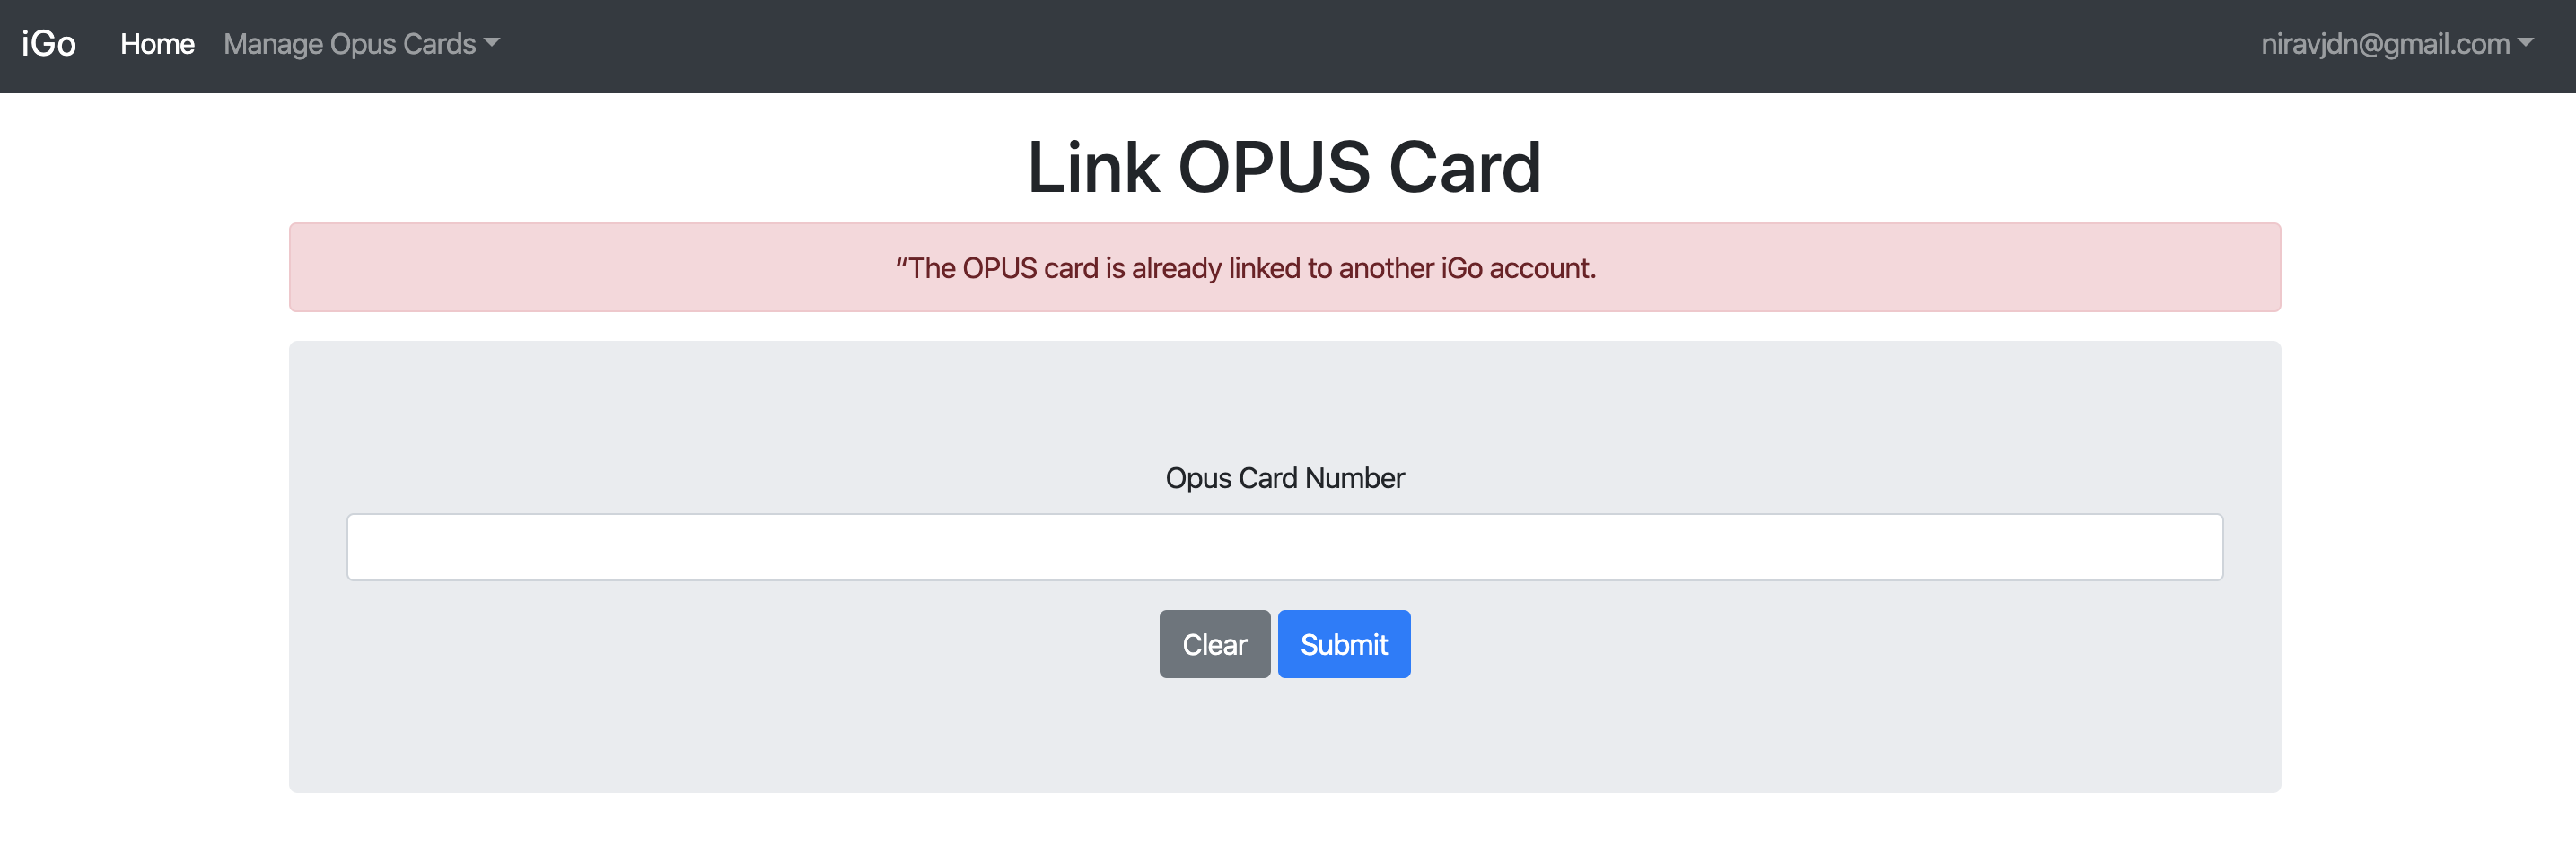
\includegraphics[width=1\textwidth]{images/already_linked_opus_card.png}
  \centering
  \caption{When the user enters opus card details that is already linked with another iGo account, the iGo system does not let them link that opus card in the account}
\end{figure}

\begin{figure}[H]
  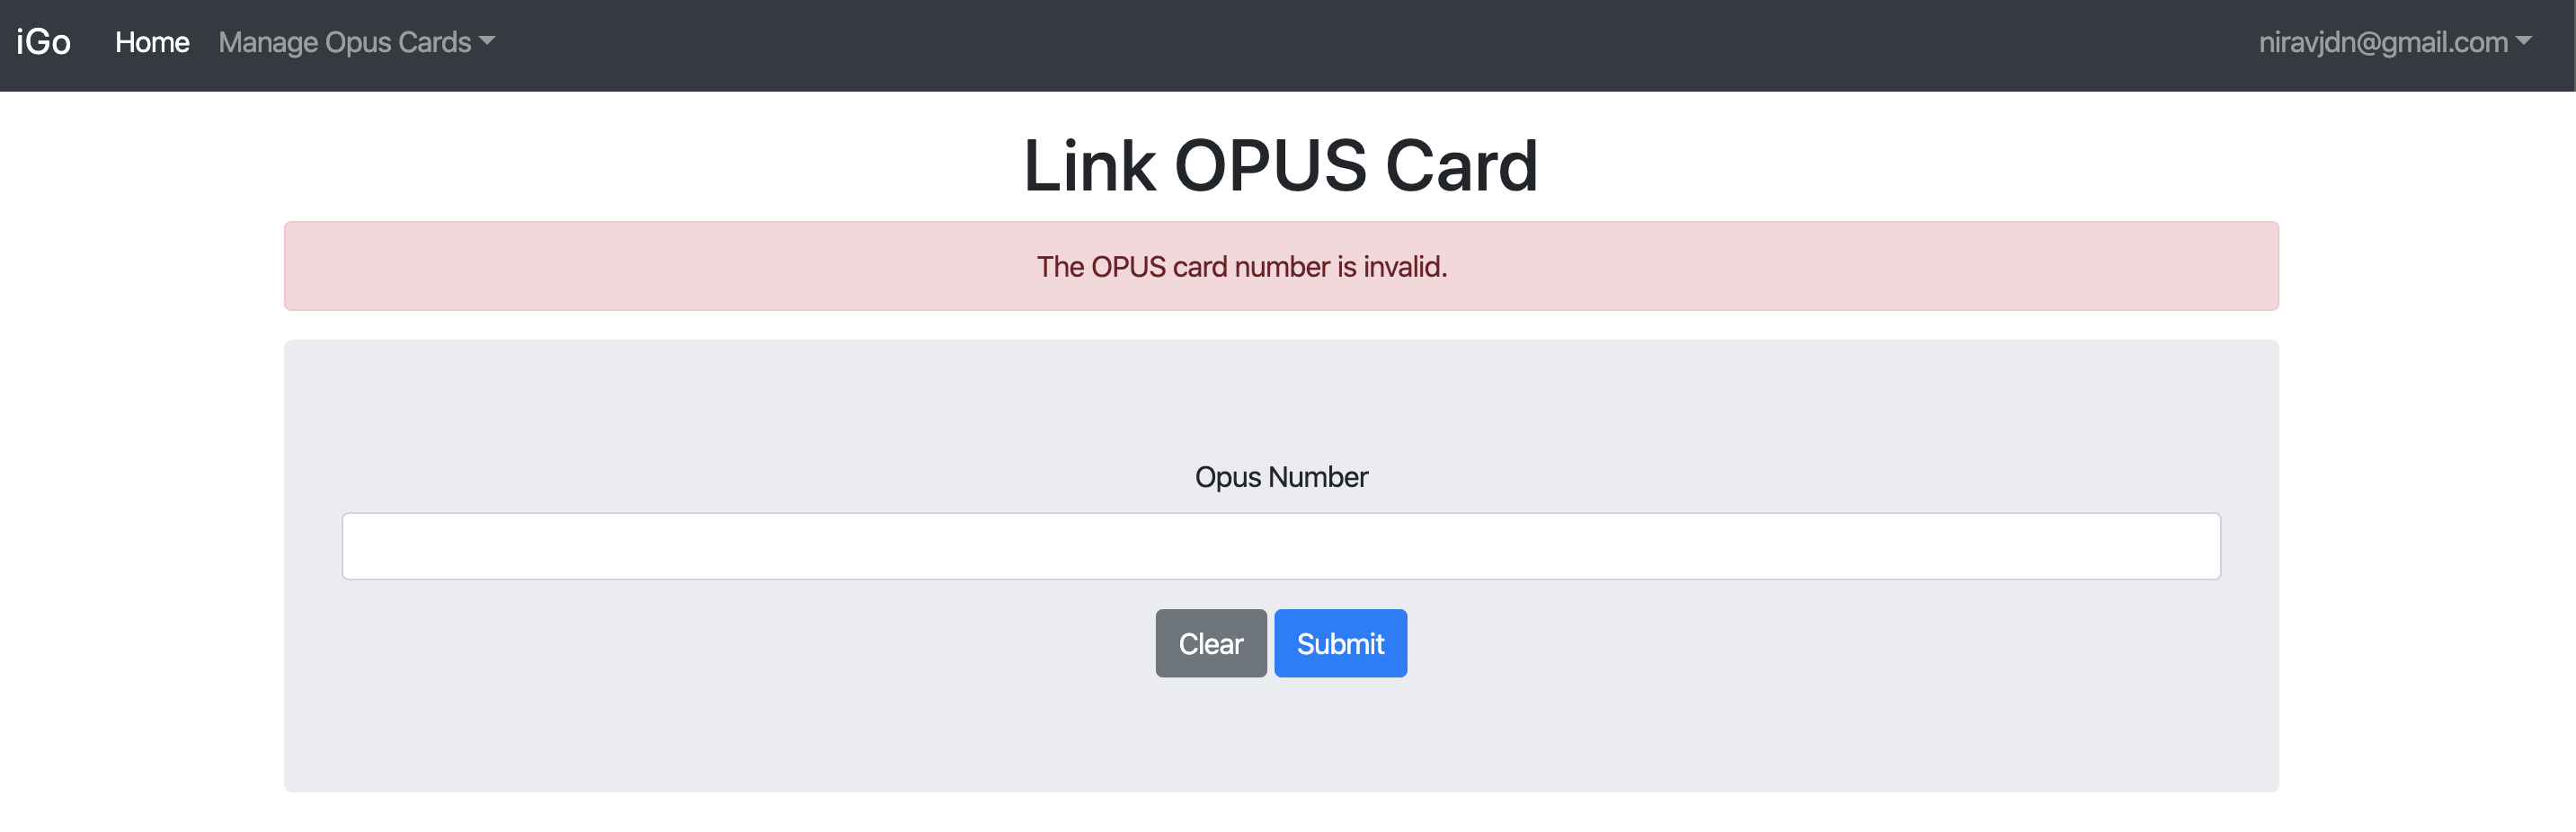
\includegraphics[width=1\textwidth]{images/invalid_opus_card_number.png}
  \centering
  \caption{When the user enter invalid Opus card details that is not in the STM database, the iGo does not let the opus card to be linked to the iGo system}
\end{figure}

\begin{figure}[H]
  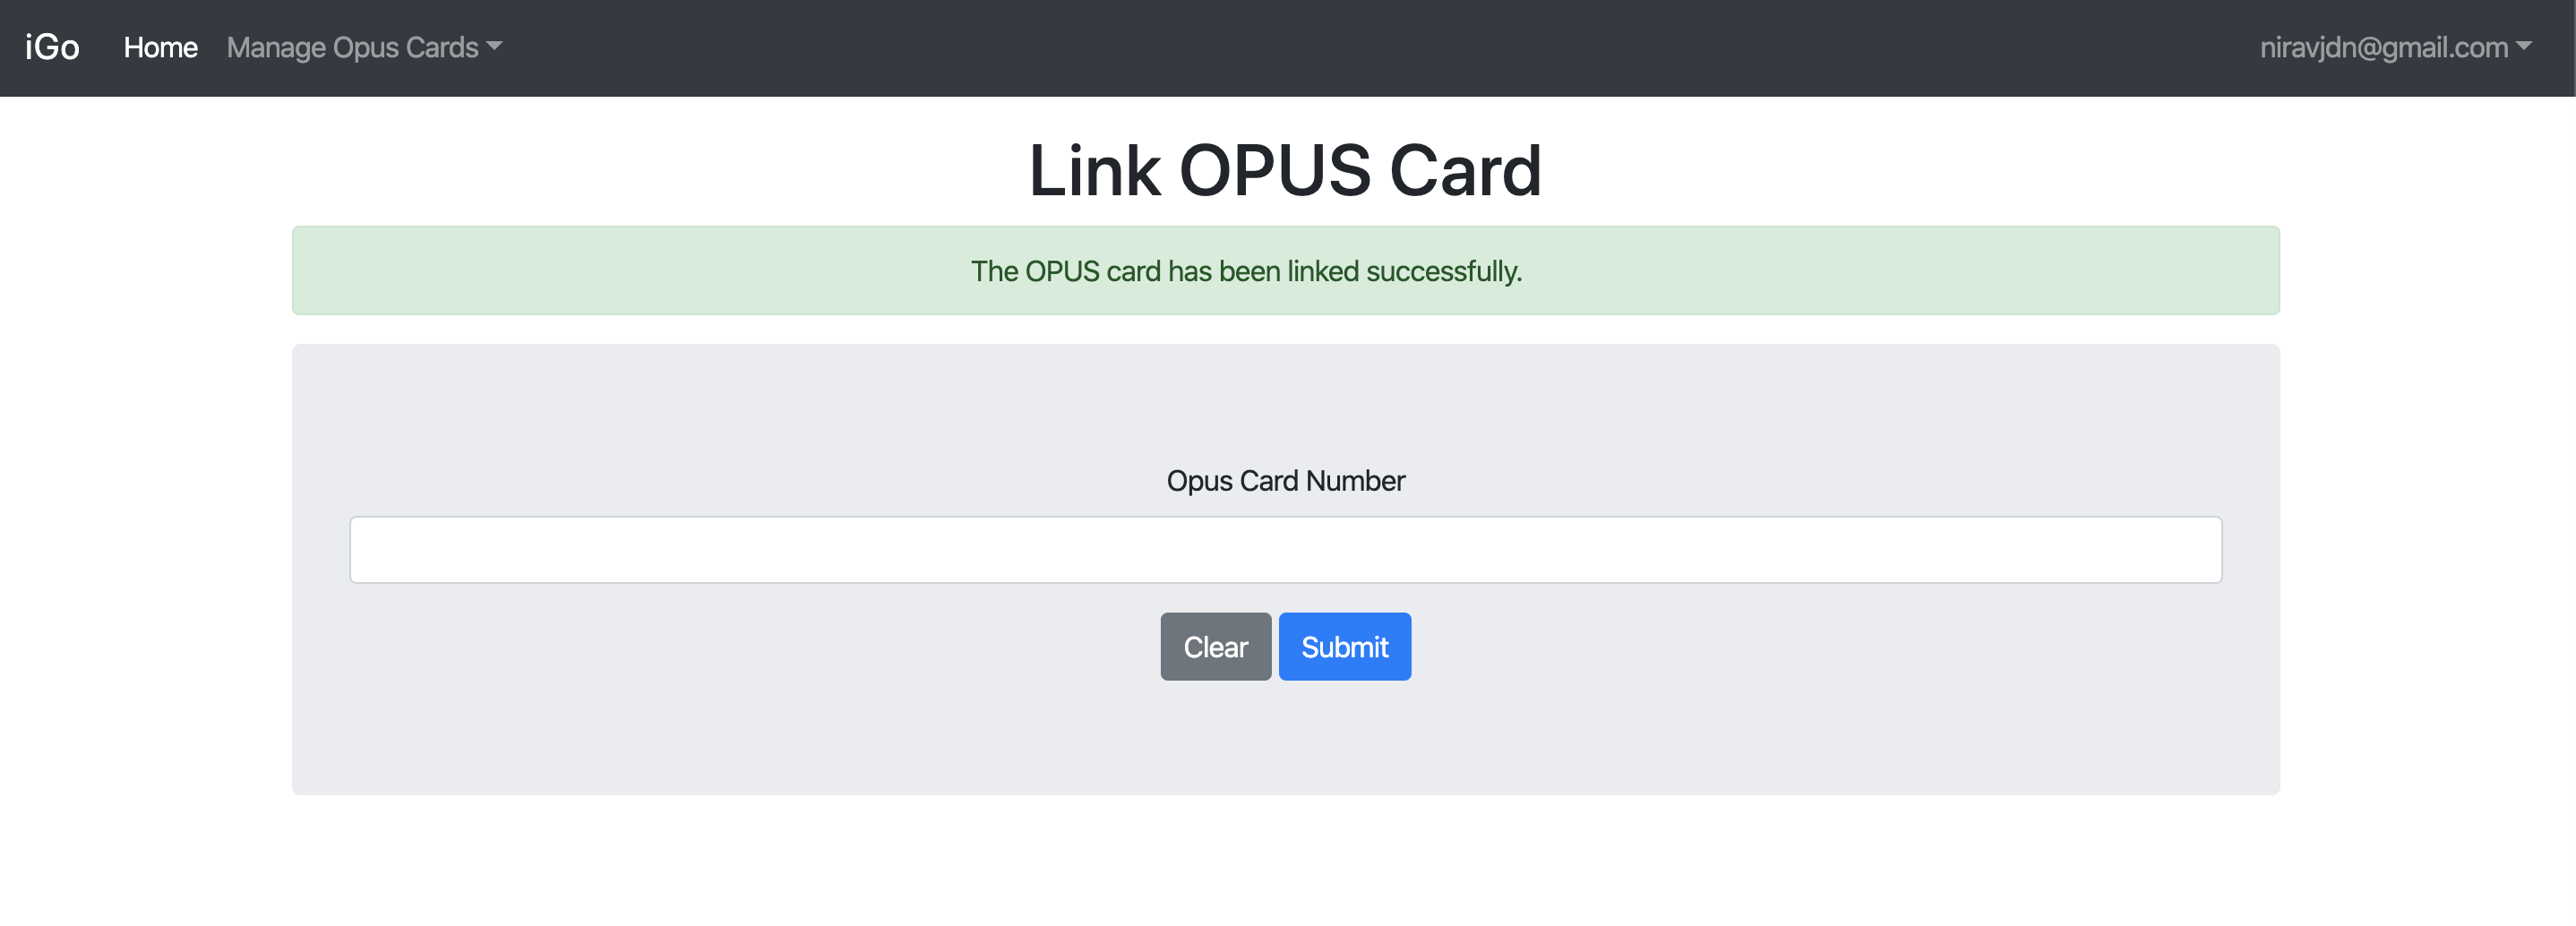
\includegraphics[width=1\textwidth]{images/link_opus_card_successful.png}
  \centering
  \caption{When the user enters valid opus card details which is valid and not linked to any other iGo account, then iGo system lets the opus card to be linked to this iGo account.}
\end{figure}


\begin{figure}[H]
  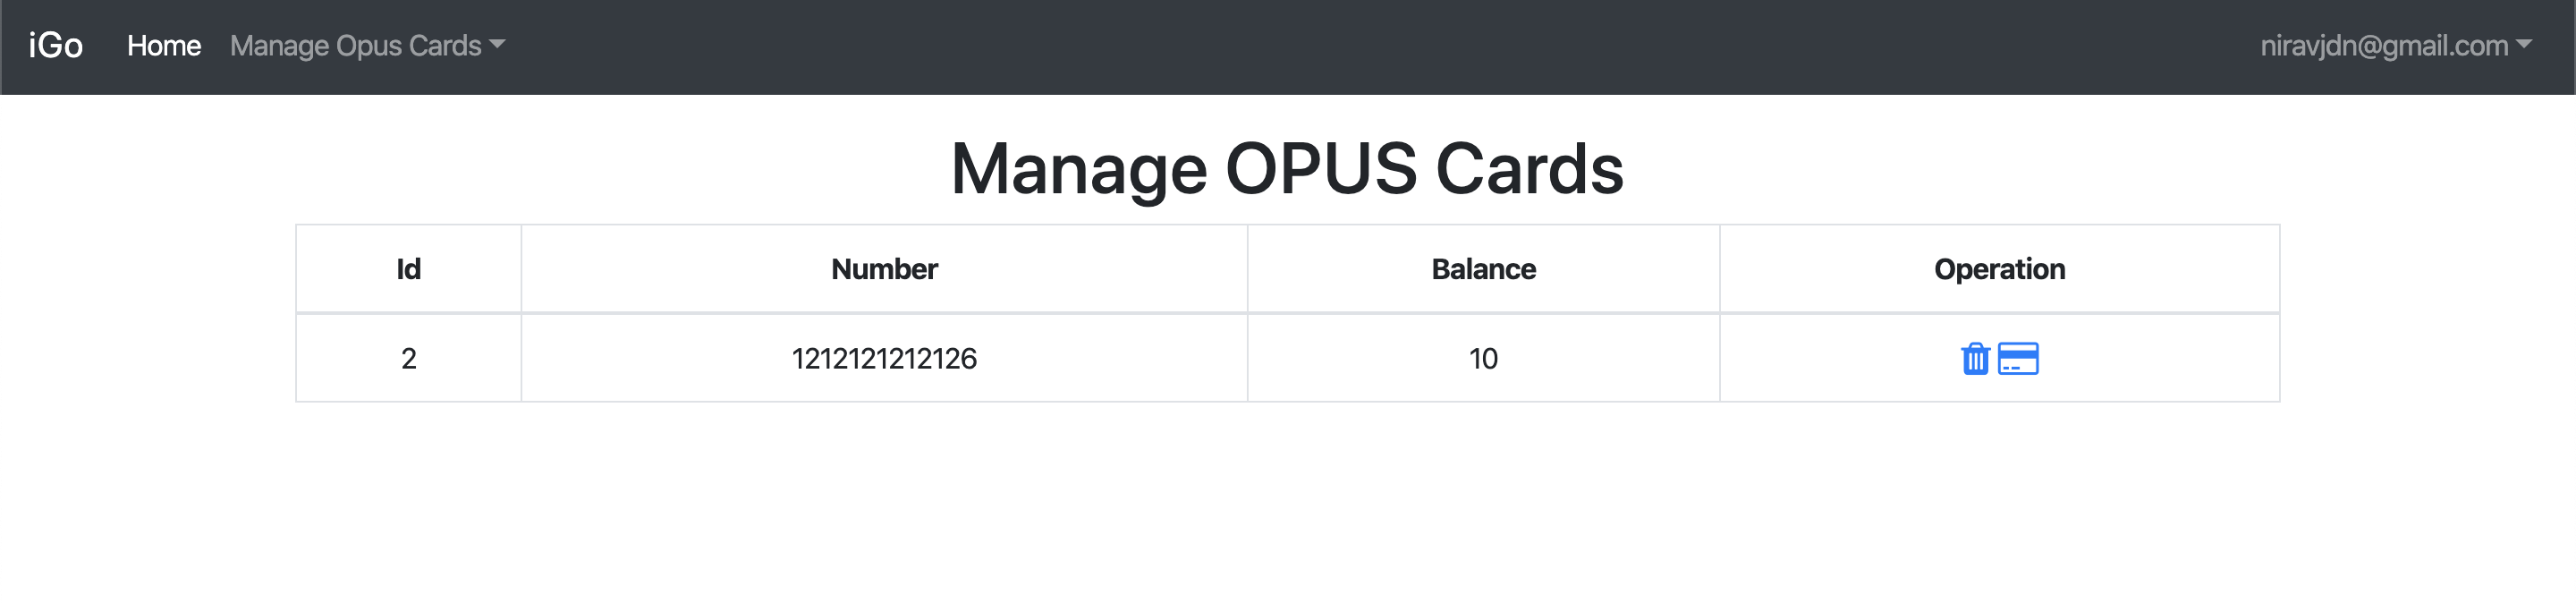
\includegraphics[width=1\textwidth]{images/manage_opus_card_page.png}
  \centering
  \caption{The Opus Card page to unlink opus card. For that user needs to click on trash icon to delete particular opus card.}
\end{figure}

\begin{figure}[H]
  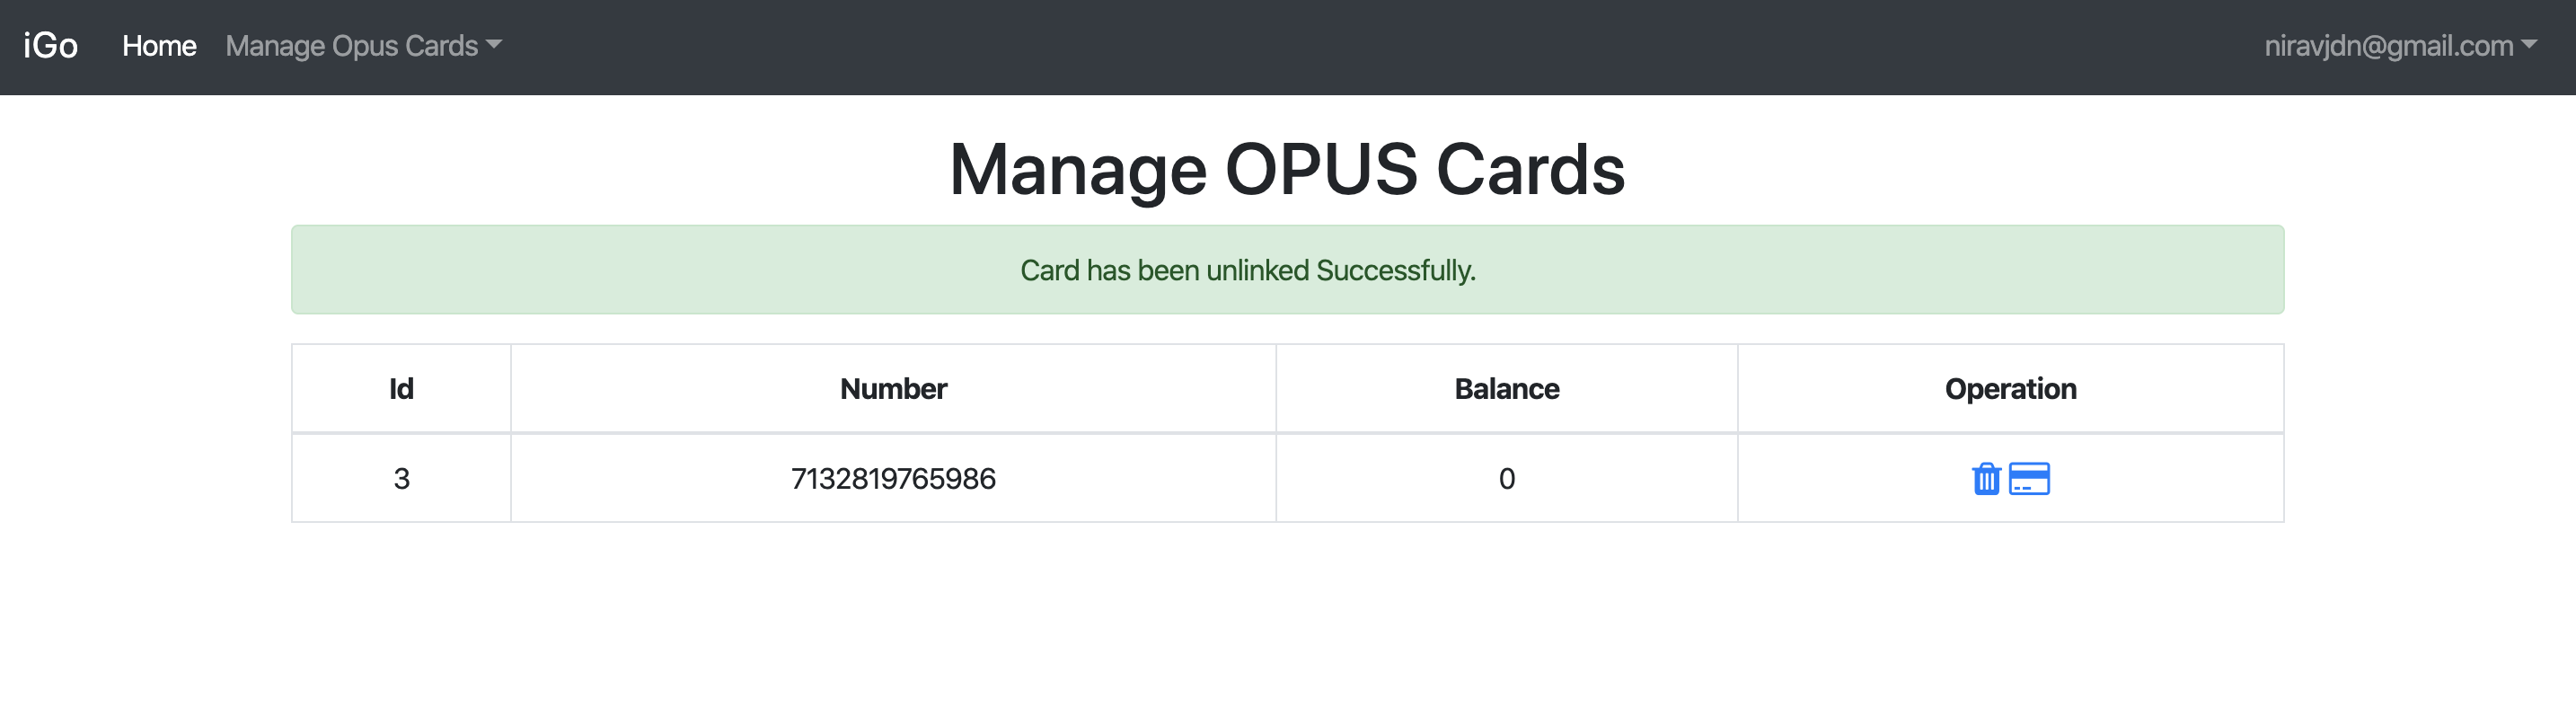
\includegraphics[width=1\textwidth]{images/unlink_opus_card.png}
  \centering
  \caption{The page showing success message that the opus card has been successfully unlinked from the account.}
\end{figure}


\section{User story 9: View OPUS Card Balance}
The existing igo User can see balance for each linked opus card to his/her account.

\begin{figure}[H]
  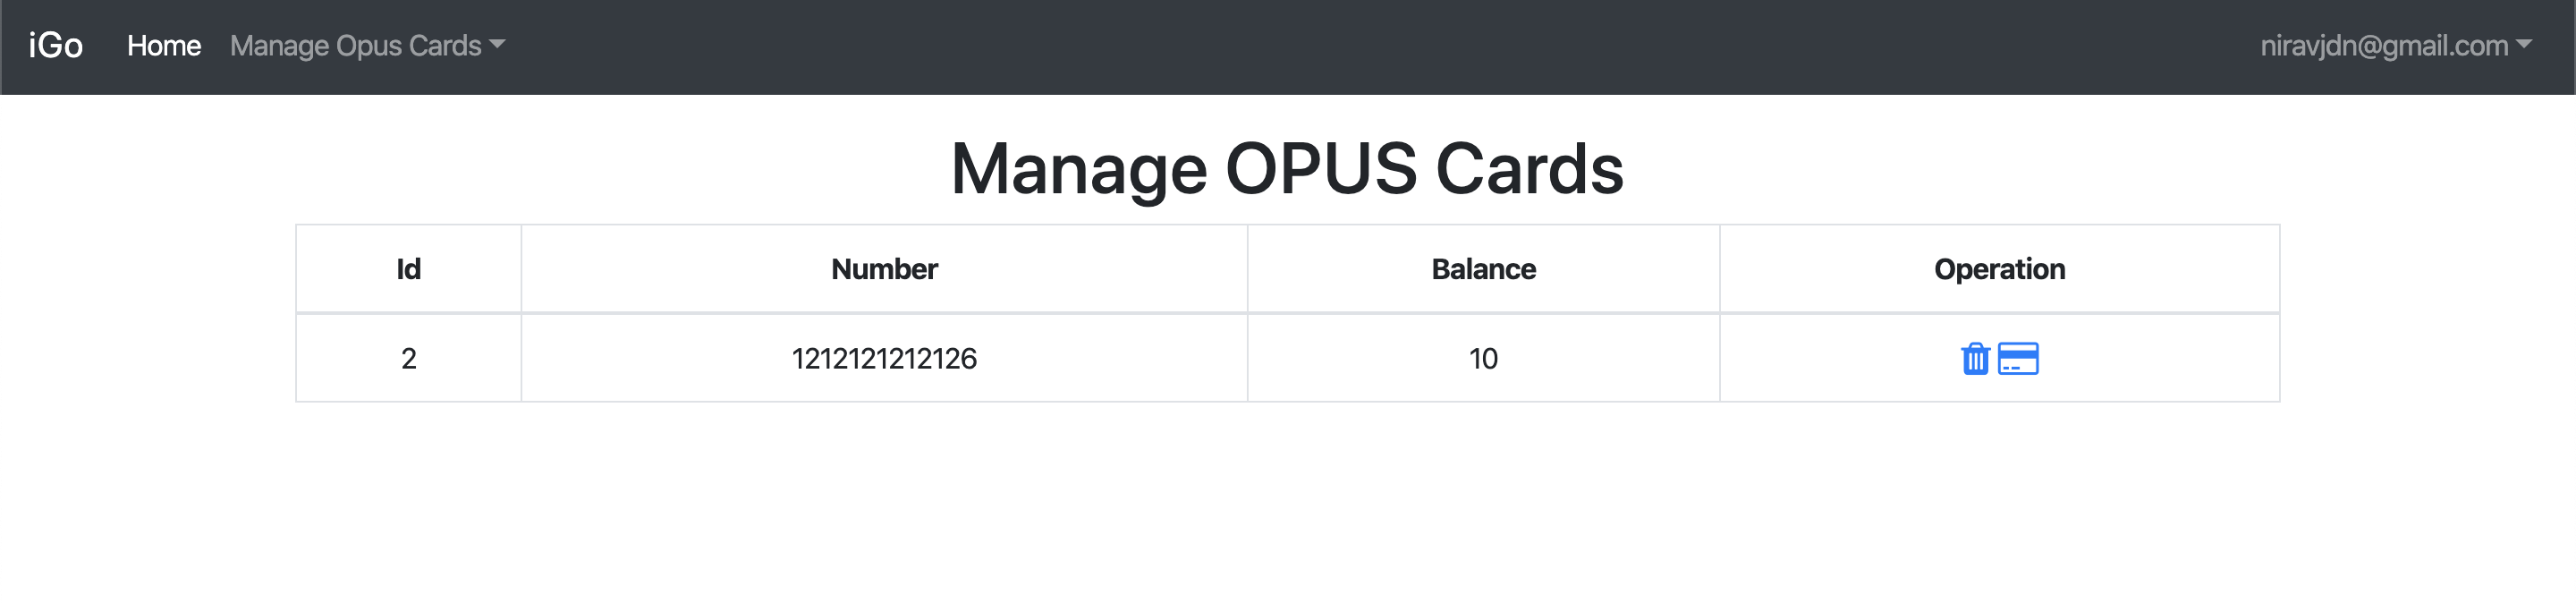
\includegraphics[width=1\textwidth]{images/manage_opus_card_page.png}
  \centering
  \caption{The page to see OPUS Card details including its balance.}
\end{figure}

\section{User story 10: Load OPUS Card}
The existing iGo User wants to load his OPUS Card using online payment via VISA/MasterCard.

\begin{figure}[H]
  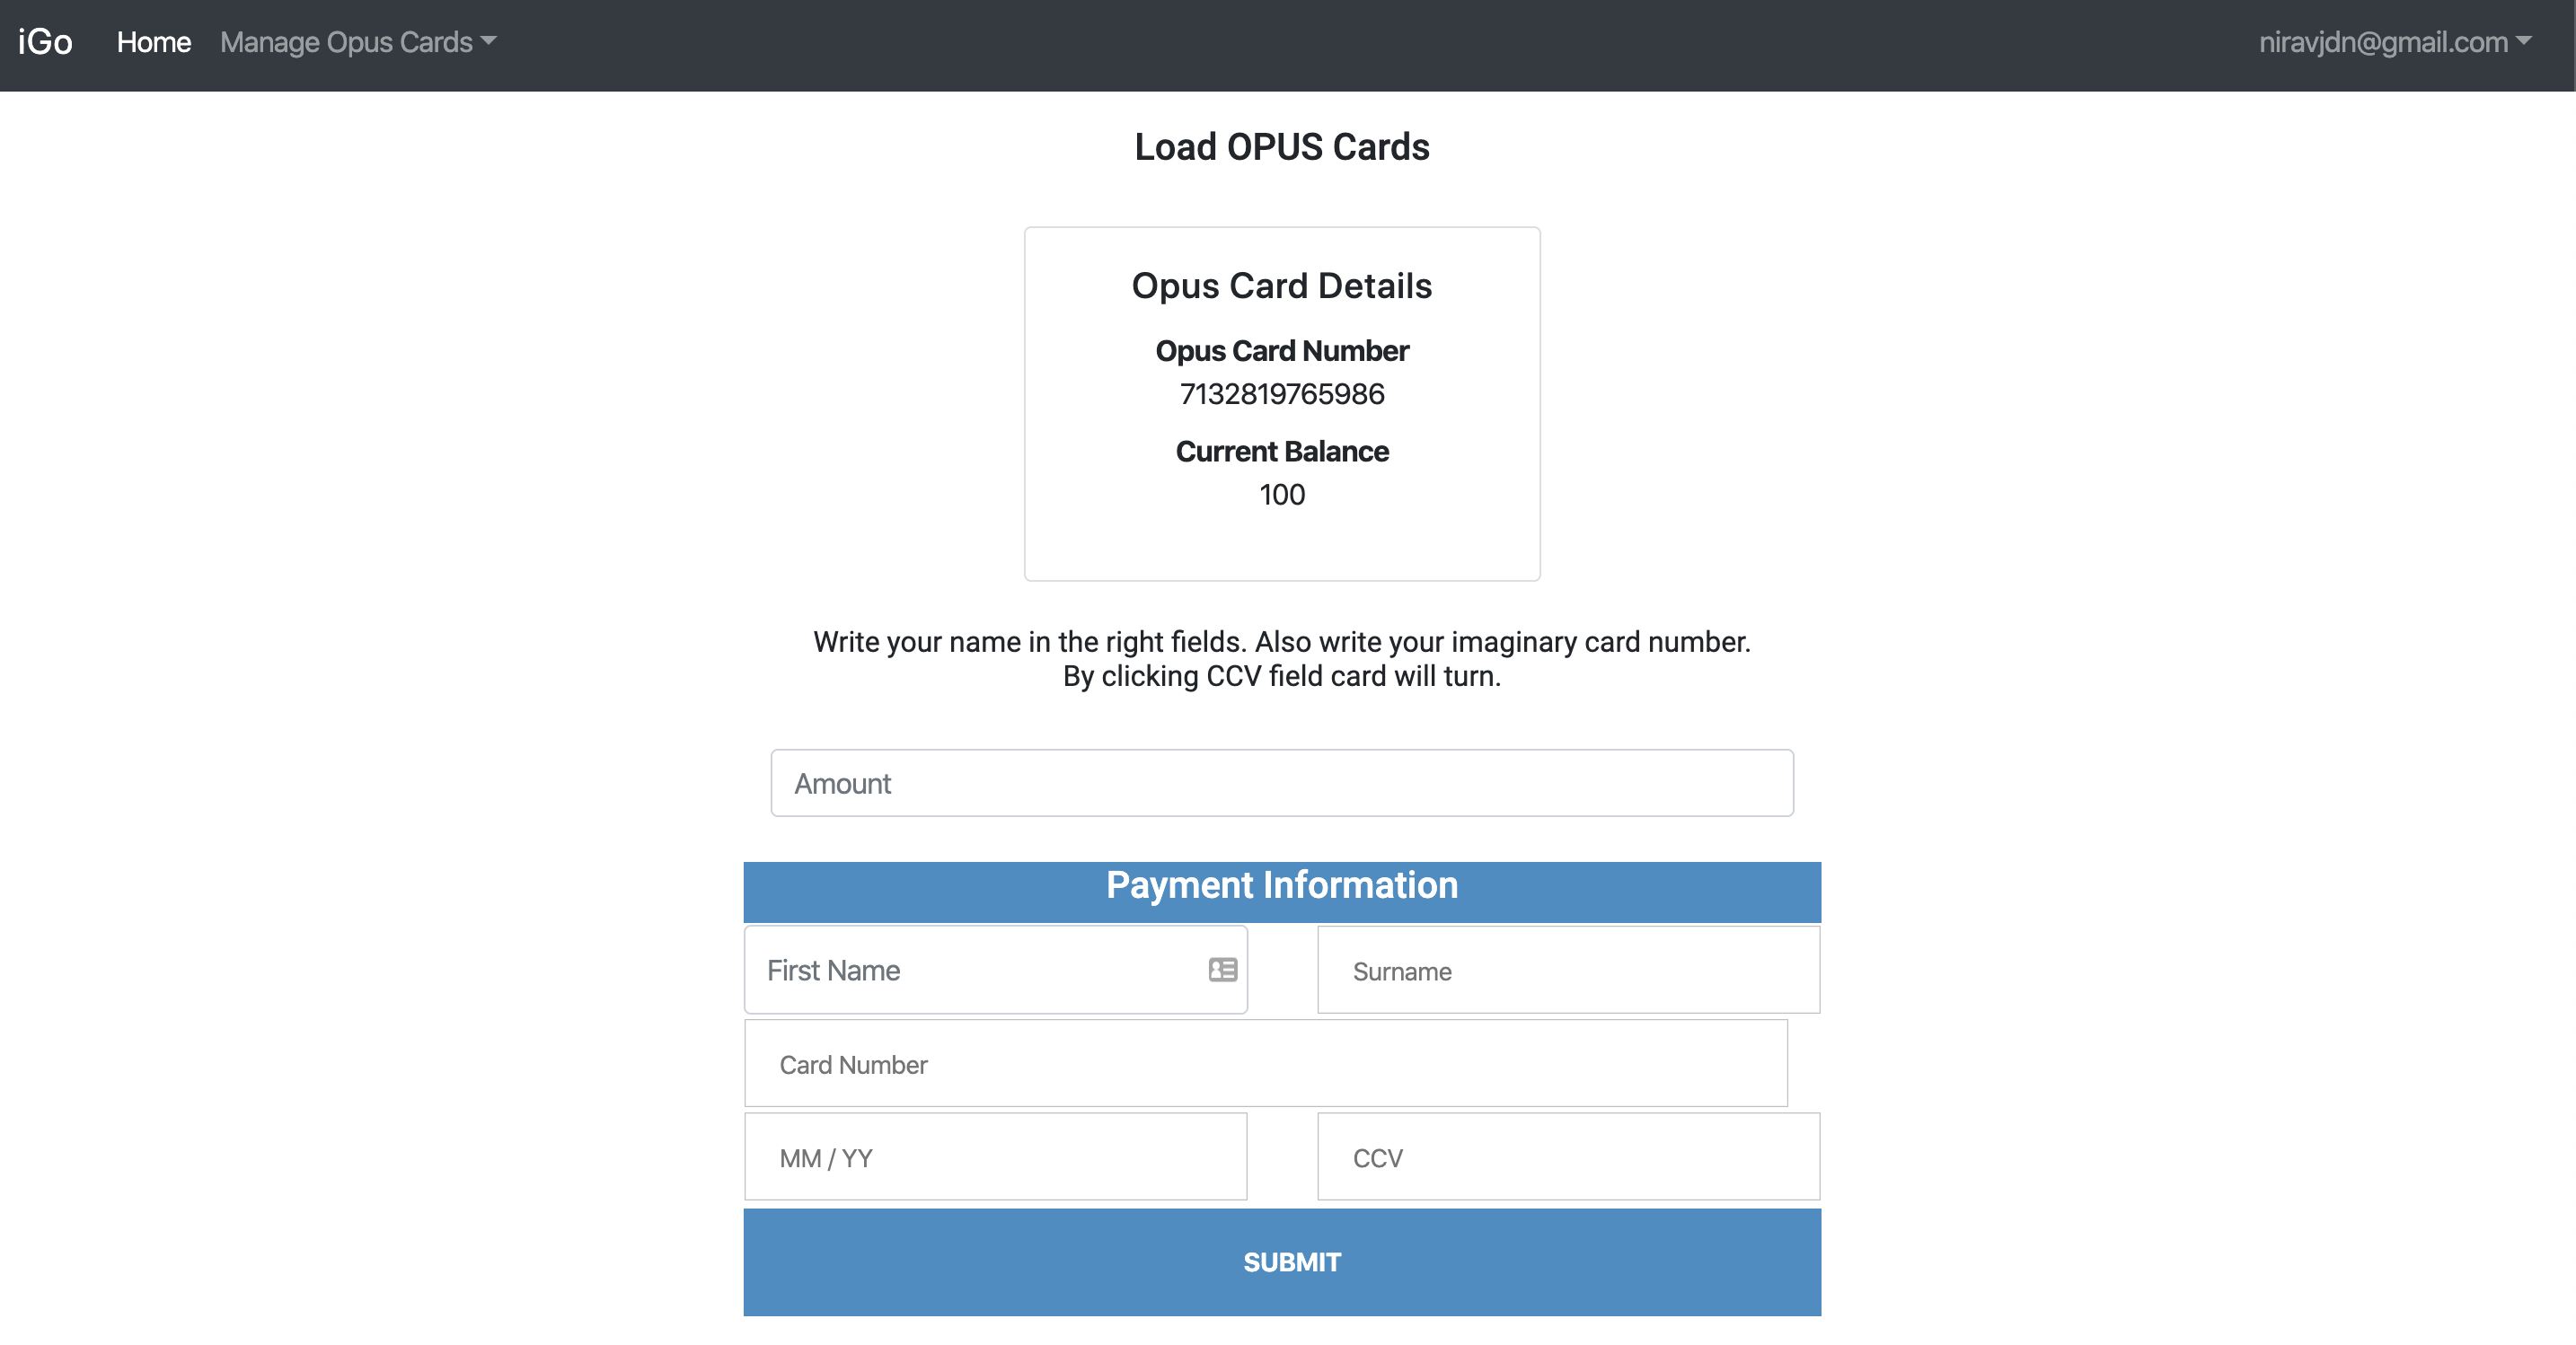
\includegraphics[width=1\textwidth]{images/load_opus_card_page.png}
  \centering
  \caption{The web page to load OPUS Card.}
\end{figure}

\begin{figure}[H]
  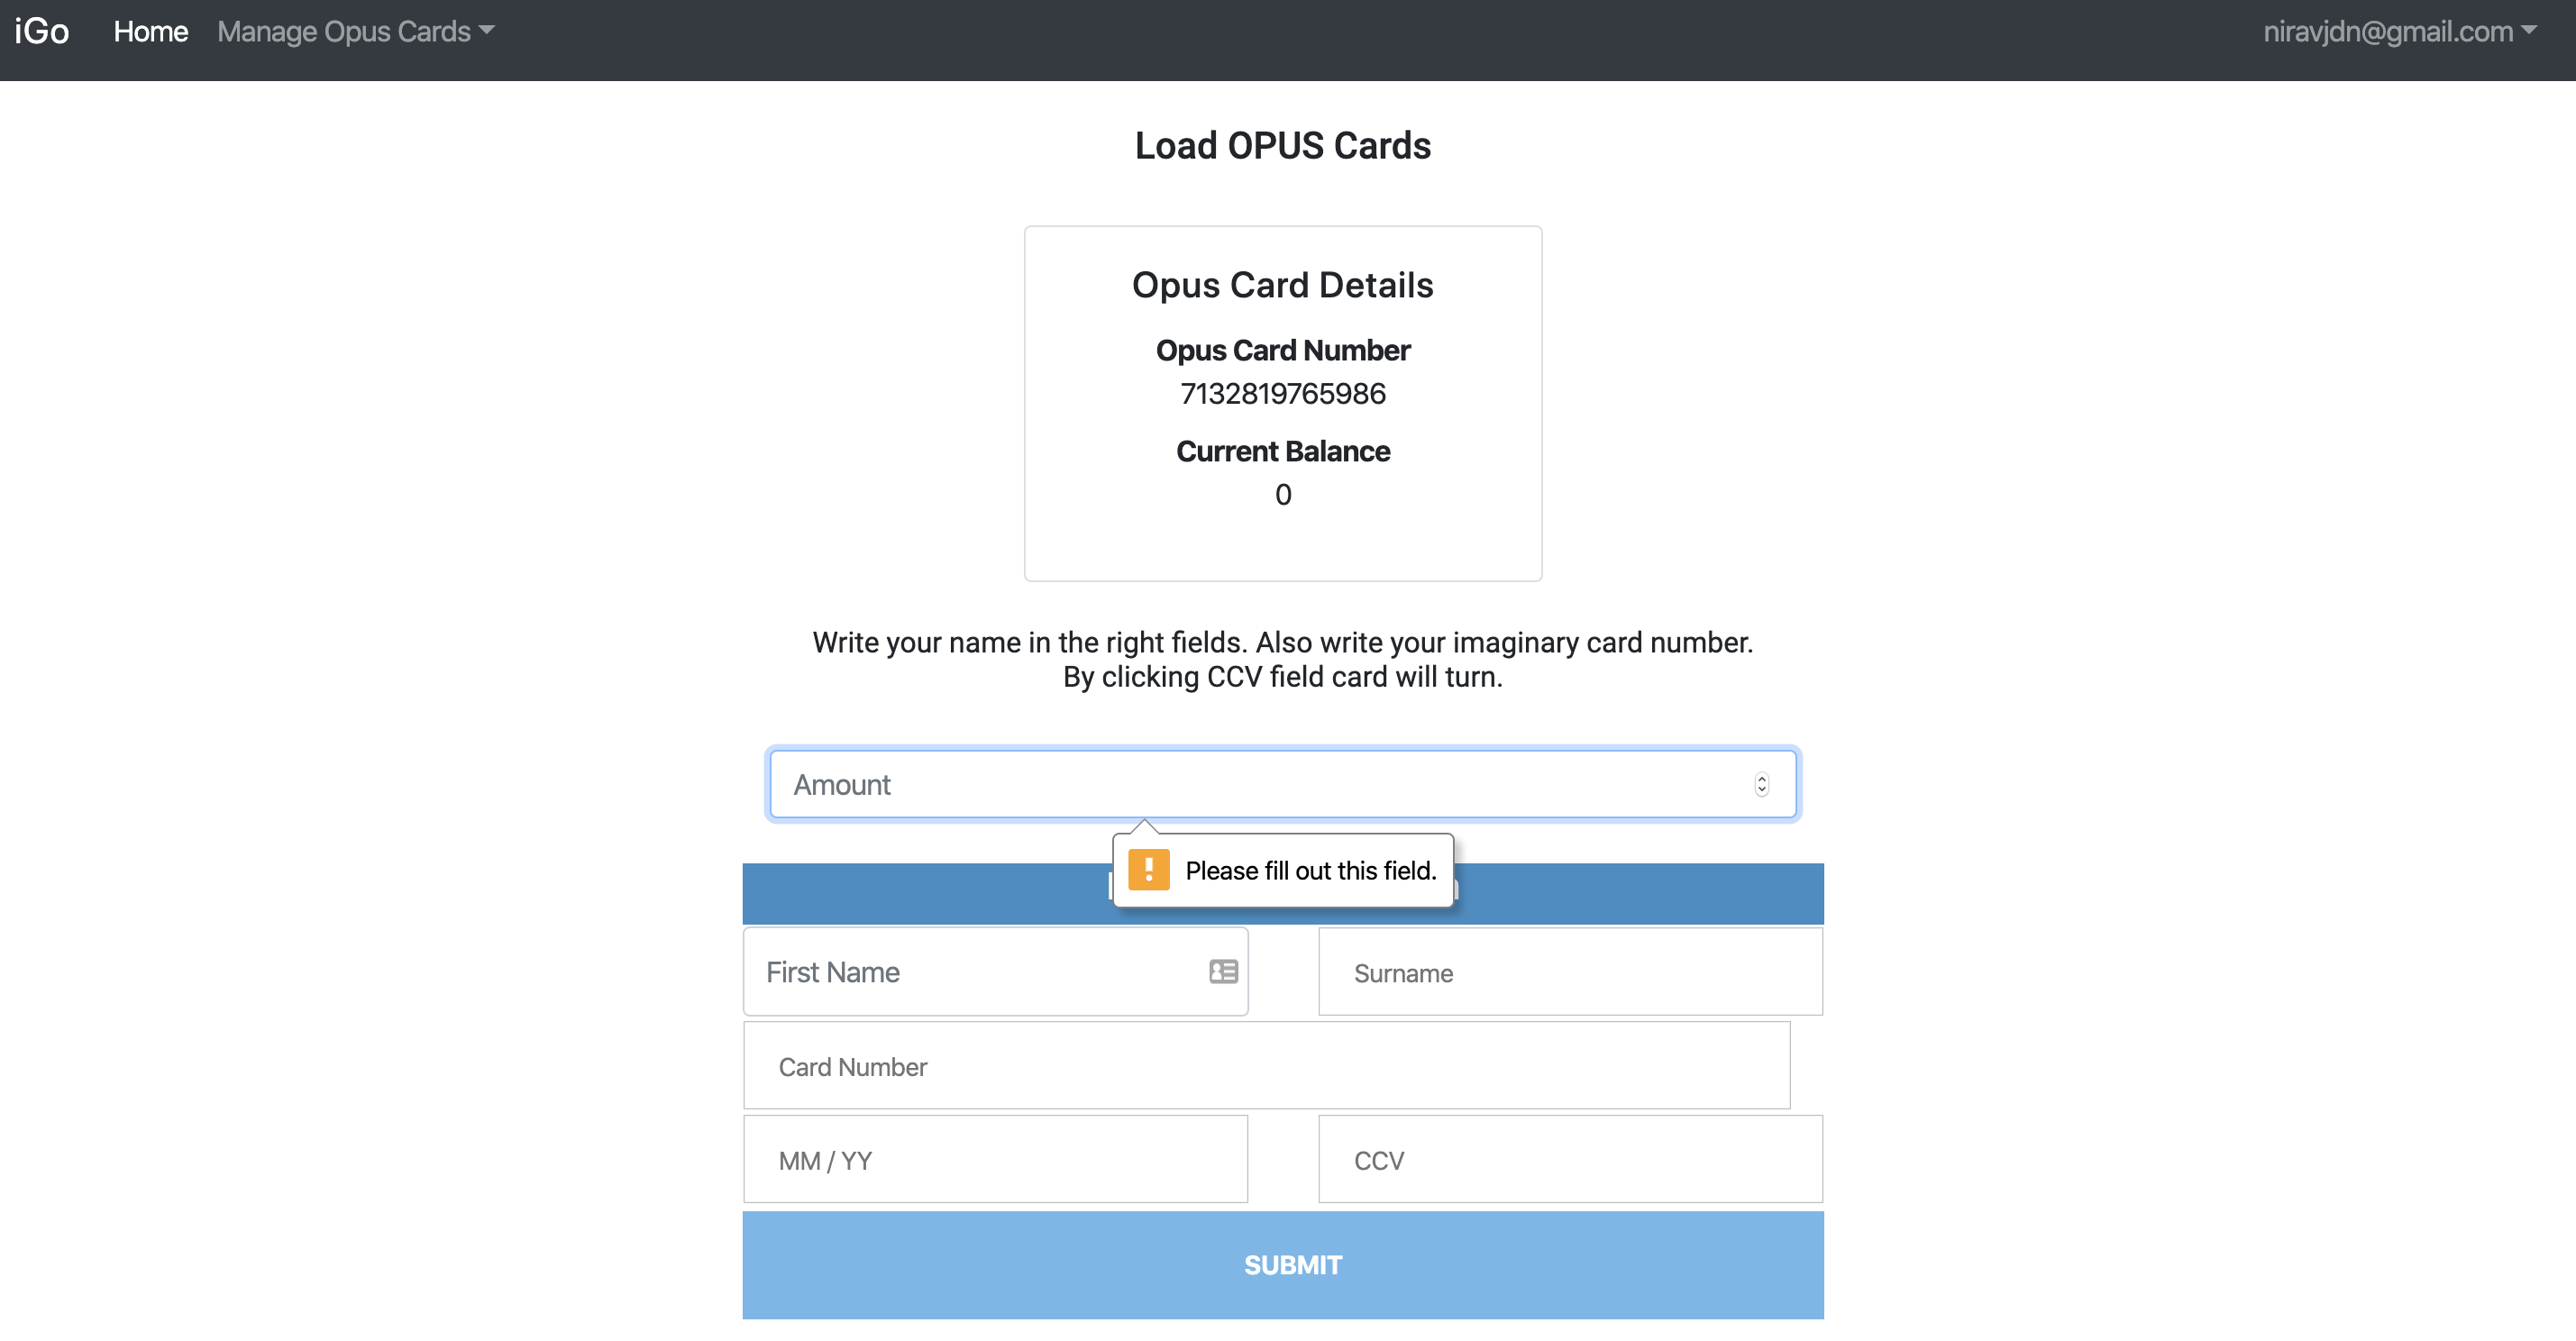
\includegraphics[width=1\textwidth]{images/opus_card_load_page.png}
  \centering
  \caption{if user does not fill the certain information which is required to process payment, user is shown message to fill the required information first and then process.}
\end{figure}


\begin{figure}[H]
  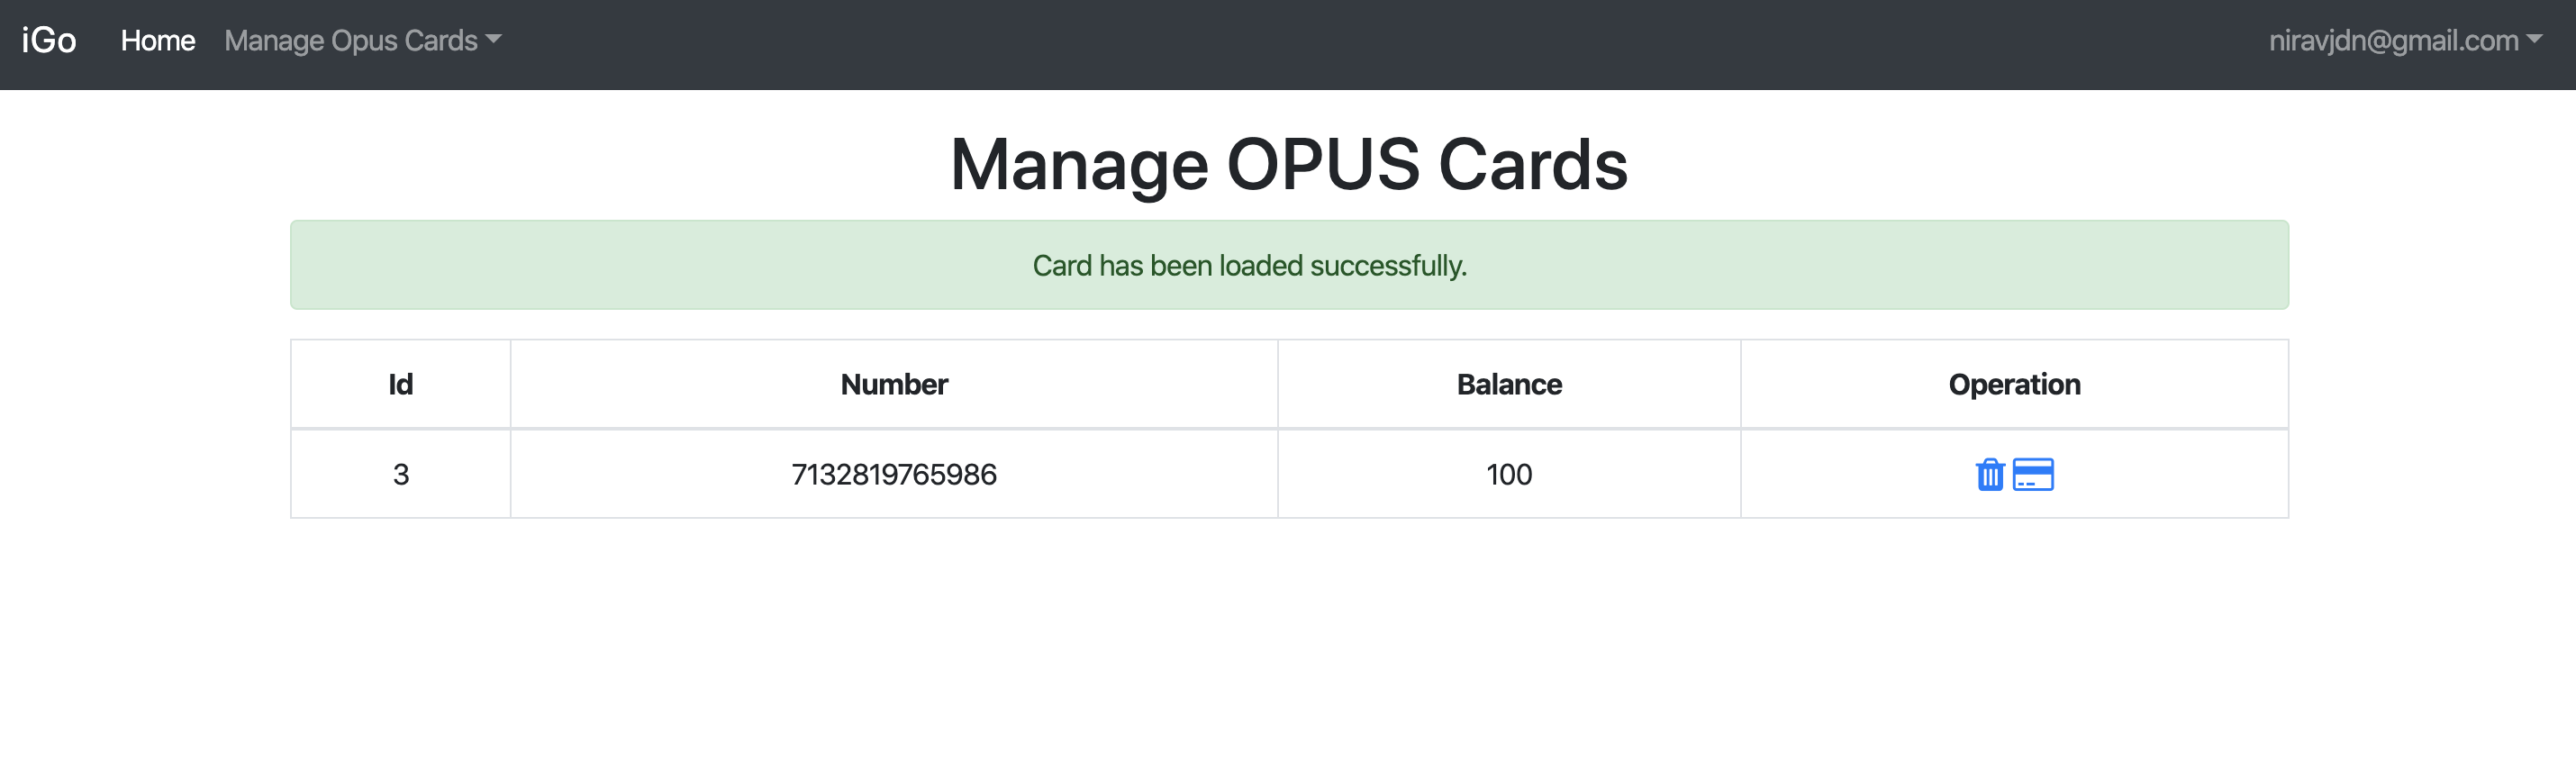
\includegraphics[width=1\textwidth]{images/opus_card_load_successful.png}
  \centering
  \caption{The message showing that card has been loaded and its updated balance.}
\end{figure}



\newpage
\chapter{Team Contribution}

\begin{center}
\begin{tabular}{ | m{20em} | m{8cm}| } 
\hline
Chapter 1 : Introduction & Nirav Patel,Rohan Deepak Paspallu,Jingya Pan,
Divya Pandit,Koshaben Patel\\ 
\hline
Chapter 2: User Stories & Nirav Patel,Rohan Deepak Paspallu,Jingya Pan,
Divya Pandit,Koshaben Patel\\ 
\hline
Chapter 3: Persona & Nirav Patel,Rohan Deepak Paspallu,Jingya Pan,
Divya Pandit,Koshaben Patel\\ 
\hline
Chapter 4: Traceability Matrix & Nirav Patel,Rohan Deepak Paspallu,Jingya Pan,
Divya Pandit,Koshaben Patel\\ 
\hline
Chapter 5: Implementation & Nirav Patel,Rohan Deepak Paspallu,Jingya Pan,
Divya Pandit,Koshaben Patel\\ 
\hline
\end{tabular}

\vspace*{0.5in}
\begin{tabular}{ | m{5em} | m{5cm}| m{5cm}| } 
\hline
User Story # & Suggested By & Implemented By \\
\hline
7, 8 & Nirav & Rohan \\
\hline
3, 4 & Kosha & Nirav \\
\hline
5, 6 & Jingya & Kosha \\
\hline
9 & Divya & Jingya \\
\hline
1, 2, 10 & Rohan & Divya \\
\hline
\end{tabular}

\end{center}


\newpage
\printbibliography
\newpage
\printglossary

\end{document}